%%%%%%%%%%%%%%%%%%%%%%%%%%%%%%%%%%%%%%%%%%%%%%%%%%%%%%%%%%%%%%%%%%
%%    Template for academic works at TU Berlin                  %%
%%    -------------------------------------------------------   %%
%%                 Created by Felix Reich, M.Sc.                %%
%%                    UTF-Version, status (2013)                %%
%%                                                              %%
%%  Operating the template using the files:                     %%
%%   - Project settings (Title, Name, Date, ...)                %% 
%%   - Commands (Custom and predefined macros)                  %%
%%   - Hyphenation (For words that are incorrectly hyphenated)  %%
%%   - Glossary (= dictionary)                                  %%
%%   - Symbols (Formula symbols for the directory)              %%
%%   - Abbreviations (For the list of abbreviations)            %%
%%   - FrontMatter (Table of contents, title page, ...)         %%
%%   - BodyMatter (IMPORTANT! Insert chapters from the folder   %%
%%                  Content with \include here)                 %%
%%   - BackMatter (List of figures, etc.)                       %% 
%%       IMPORTANT: Definitely customize Front and Backmatter   %%
%%       individually by commenting or uncommenting commands    %%
%%   - Appendix (if available, insert with \include here)       %%
%%                                                              %%
%%  Three different KOMA classes can be used:                   %%
%%  - scrartcl -scrreprt (standard) -scrbook                    %%
%%  To change, in the file Class adjust the documentclass and   %%
%%  the logical switch accordingly.                             %%
%%                                                              %% 
%%  It is recommended to modify the other files as little as    %%
%%  possible. Newcomers to academic typesetting should study    %%
%%  the documents in the Help directory to achieve an           %%
%%  aesthetically pleasing result.                              %%
%%                                                              %%
%% Those who want to include eps files must pass to pdflatex    %%
%%    --shell-escape for tetex or texlive or                    %%
%%    --enable-write18 for miktex.                              %%
%%                                                              %%
%% To use the directories Index, Glossary, Abbreviations,       %%
%% and Symbols, respectively, makeindex must be called with:    %%
%% -s "Index/Index.ist -i Document.idx -o Document.ind          %%
%% -s Document.ist -t Document.glg -o Document.gls Document.glo %%
%% -s Document.ist -t Document.alg -o Document.acr Document.acn %%
%% -s Document.ist -t Document.slg -o Document.sym Document.sbl %%
%%%%%%%%%%%%%%%%%%%%%%%%%%%%%%%%%%%%%%%%%%%%%%%%%%%%%%%%%%%%%%%%%%
% cd C:\CloudStorage\tubCloud\13. MA\Latex\Thesis
% Index: 	makeindex -s "Index/Index.ist -i Document.idx -o Document.ind
% Acronym: 	makeindex -s Document.ist -t Document.alg -o Document.acr Dokument.acn
% Glossar:  makeindex -s Document.ist -t Document.glg -o Document.gls Dokument.glo


% Basic Settings
% Document settings are made here. Deeper layout settings follow separately.

% Also possible here, among others:
% Number of columns (onecolumn, twocolumn)
% Chapters start only on right-hand pages or on any (openright, openany)
% Beginning of paragraphs (parindent, halfparskip, parskip)

\documentclass[
headings=normal,                        % Headings size (options: small, normal, and big)
captions=tableheading,                  % Format table captions as headings
bibliography=totoc,                     % Adds the bibliography to the table of contents
listof=totoc,                           % Adds the other lists to the table of contents
index=totoc,                            % Also adds the index to the table of contents
draft=false                             % Figures are set. With draft=true, figures are only available as frame dummies
]{scrreprt}                             % Choose from scrartcl, scrreprt, and scrbook !!! Definitely adjust the switch below !!!

% Logical switches for document class
\def\typeScrartcl{1}  % For scrartcl
\def\typeScrreprt{2}  % For scrreprt
\def\typeScrbook{3}   % For scrbook

% !! Set the switch here so that the template works correctly !!
\let\doctype=\typeScrreprt


% Project Definitions
% Front matter
\newcommand*{\Titel}{Design and Control of a Multi-Joint Two-Wheeled Inverted Pendulum Robot for Agile Motion Learning}
\newcommand*{\Untertitel}{Exploiting Similarity for Data-Driven Input Trajectory Transfer}
% Header title
\newcommand*{\HeaderTitel}{Design and Control of a Multi-Joint Two-Wheeled Inverted Pendulum Robot}

% Main author
%\newcommand*{\Autor}{Philipp Drebinger}
\newcommand*{\AutorMatrikelNr}{10044038}

\newcommand{\Autor}%                % Author's name
{Mohamed Barakat}
\newcommand{\Matrikelnummer}%       % Matriculation number
{10044038}
\newcommand{\Datum}%                % Submission date
{15. January 2024}

\newcommand{\TitelDerArbeit}%       % Title of the work
{Design and Control of a Multi-Joint Two-Wheeled Inverted Pendulum Robot for Agile Motion Learning}

\newcommand{\Kennnummer}%           % Here enter the identifier number of the work. You will receive this shortly before submission from your supervisor
%{M-MM/JJJJ-XXXXX}
{15-01/2024-1234}
%{M-Month/Year-Number}

\newcommand{\ArtDerArbeit}%         % Type of work. Please enter whether Master's thesis, Bachelor's thesis, or study thesis
{Master's thesis} 
%{Bachelor's thesis}
%{Study thesis}

\newcommand{\Erstpruefer}%          % Enter the name of the first examiner here
{Prof. Dr.-Ing. Thomas Seel}
\newcommand{\Zweitpruefer}%         % Enter the name of the second examiner here
{Prof. Dr.-Ing. Firstname Lastname}
\newcommand{\Betreuer}%             % Enter the name of the research assistant supervisor here
{Dustin Lehmann}

% Manually set date with location
%\newcommand*{\Datum}{Berlin, the 16th of March 2023}

% University, faculty, institute, and department
\newcommand*{\Uni}{Technische Universit\"at Berlin}
\newcommand*{\Fakultaet}{Fakult\"at IV}
\newcommand*{\Institut}{Institut f\"ur Energie- und  Automatisierungstechnik}
\newcommand*{\Fachgebiet}{Control Systems Group}

% Professor and supervisor
\newcommand*{\Professor}{Prof. Dr.-Ing. J\"org Raisch}
\newcommand*{\ProfessorII}{Prof. Dr.-Ing. Clemens G\"uhmann}
\newcommand*{\BetreuerA}{M.Sc. Dustin Marlon Lehmann}
\newcommand*{\BetreuerB}{}

% Additional authors
\newcommand*{\AutorB}{}
\newcommand*{\AutorBMatrikelNr}{}
\newcommand*{\AutorC}{}
\newcommand*{\AutorCMatrikelNr}{}
\newcommand*{\AutorD}{}
\newcommand*{\AutorDMatrikelNr}{}
\newcommand*{\AutorE}{}
\newcommand*{\AutorEMatrikelNr}{}

% Group indication or just "submitted by:"
\newcommand*{\Gruppe}{by}

% Setting the print version: print or PDF view only
\def\typeDrucken{1}  % For printing (do not change)
\def\typePDFonly{2}  % For PDF-only use (do not change)
% Set the appropriate switch here! =\typeDrucken or =\typePDFonly
\let\pdftype=\typeDrucken

% Definition of whether to set single or double-sided
\def\typeOnepage{1}  % For single-sided setting
\def\typeTwopage{2}  % For double-sided setting
% Set the appropriate switch here! =\typeOnepage or =\typeTwopage
\let\pagetype=\typeOnepage

% Binding correction at the inner margin
\newlength{\bindCorrection}                % Declaration, do not change
\setlength{\bindCorrection}{0cm}           % Assignment, can be changed

% PDF output version via Minor number => 1.x
\pdfminorversion=5


% CUSTOM
% Colorful: 1, Plain: 2
\def\colorfulLayout{1}


% Packet Definitions
% Settings for input (character set, language, ...)
\input{Settings/Eingabe}

% Typesetting settings
\input{Settings/Satzeinstellungen}

% Various helper packages
% Paket für schnellen Beispieltext zum Füllen
\usepackage{blindtext}
% Aus der Hilfe:
% \blindtext creates some text,
% \Blindtext creates more text.
% \blinddocument creates a small document with sections, lists...
% \Blinddocument creates a large document with sections, lists...

% etools

% Weitertes Macro-Paket. Zwar depreciated, dennoch benötigt, da es in Skripten Kommandos auflöst
\usepackage{ifthen}
% Bsp: \ifthenelse{\equal{\kommando1}{\kommando2}}{true}{false}

% Ermöglicht das Verwenden von Listen mit kleineren vertikalen Abständen
%\usepackage{mdwlist}
%% Statt itemize einfach itemize* verwenden. Analog dazu existiert enumerate* und description*
%% Diese Umbegungen erlauben auch Unterbrechungen, z. B.  mit \suspend{itemize*} bla bla \resume{itemize*}
% stattdessen \begin{itemize}[noitemsep,topsep=0pt], bzw \begin{enumerate}[resume*]
\usepackage[inline]{enumitem}

% for todolists
\newlist{todolist}{itemize}{2}
\setlist[todolist]{label=$\square$,noitemsep, topsep=0pt}
\usepackage{pifont}
\newcommand{\cmark}{\ding{51}}%
\newcommand{\xmark}{\ding{55}}%
\newcommand{\done}{\rlap{$\square$}{\raisebox{2pt}{\large\hspace{1pt}\cmark}}%
\hspace{-2.5pt}}
\newcommand{\wontfix}{\rlap{$\square$}{\large\hspace{1pt}\xmark}}
% EXAMPLE CODE FOR TODO LIST IN S TODO BOX ENVIRONMENT:
%\begin{todobox}
%  \begin{todolist}
%  \item[\done] Frame the problem
%  \item Write solution
%  \item[\wontfix] profit
%  \end{todolist}
%\end{todobox}



% Ermöglicht erweiterte Referenzen. Soweit angepasst, dass schöne Makros möglich sind (siehe Kommando-Definitionen)
\usepackage[english]{varioref}
\renewcommand*{\reftextfaraway}[1]{auf S.\,\pageref{#1}}%
\renewcommand*{\reftextcurrent}{\unskip}%
% generell neu: \vpageref, \vref und \vref*, diese Referenzierungen geben die Seite mit an

% Ermöglichung von Unterabbildungen
%\usepackage{subfig}
%% Verwendung in figure: \subfloat[Optionaler Verzeichnistext][Unterschrift \label{sfig:bla}]{...Zeug...}
% I use subcaption
\usepackage{subcaption}
\usepackage{caption}
\captionsetup{width=.8\textwidth}

% Das normgerechte Eurozeichen
\usepackage{eurosym}
% Verwendung mit \euro

% Kommandos nach Ende einer Seite absetzen
\usepackage{afterpage} 
% Wichtigste Anwendung ist das Flushen von Floats: \afterpage{\clearpage}

 % Nassi-Schneidermann Unterstützung
\usepackage{Packets/nassi}
\setiftext{W}{F}
\nassiwidth=\textwidth
% Wichtige Befehle:
% \NSD{}
% \WHILE{Text}{} \ENDWHILE
% \ACTION{Text}

% Einrahmen von Text
\usepackage{framed}
\addtolength{\FrameRule}{1pt} % dickeren Rahmen
% Verwendung: \begin{framed} ... \end{framed}

%Comment blocks using \begin{comment} ... \end{comment}
\usepackage{comment}
%\includecomment{commentnotes} % environment to comment stuff
\excludecomment{commentnotes}

% For color boxes like todobox, notebox, etc
\usepackage[most]{tcolorbox}


% Abstrct
\usepackage{abstract}
\usepackage{lipsum}

% Layout settings
% Hier sind Layoutoptionen zu finden, die aus Übersichtsgründen nicht in der Datei "Klasse.tex" eingefügt sind

% Serifenschrift 
% Ersetzt Computer Modern mit Latin Modern, sieht aber nahezu gleich aus. Grund ist die mangelnde Unterstützung von korrekt gesetzten Umlauten und die Lesbarkeit am Monitor.
\usepackage{lmodern}

% Fügt Symbole zum Font hinzu, die in Latin Modern nicht enthalten sind, wie z. B. das Euro-Symbol
\usepackage{textcomp}

% Ersetzt die Schreibmaschinen-Schrift und verwendet Adobe Courier statt Latin Modern oder Computer Modern
\usepackage{courier}

% Optischer Randausgleich
\usepackage{microtype}
% Wenn man die Augen zukneift, kann man ohne diesem Paket bei Blocksatz auf der rechten Seite "Dellen" erkennen, da Punkte und Striche vor der virtuellen Trennlinie gehalten werden. Dieses Paket ermöglicht kleine Übertretungen, die das optische Bild verbessern.

% Setzt die Schriftgröße. Ebenfalls soll die Titelseite separat gesetzt werden
\KOMAoptions{
fontsize=10pt,			% Schriftgröße. Standard = 11pt
titlepage=true			% Separat gesetzte Titelseite verwenden
}

% Verwendung des geometry Packets für die Einstellung des Papierformats / Seitenabstände / Bindekorrektur
\usepackage[
a4paper, 													% DIN A4-Papier
  inner=25mm,
  outer=25mm,
  top=25mm,
  bottom=25mm,
  heightrounded,
  marginparwidth=51pt,
  marginparsep=17pt,
  headsep=24pt,
%\ifcase\pagetype \or twoside=false \or twoside=true \fi , 	% Ein- oder zweiseitig 
bindingoffset=\bindCorrection								% Binde-Korrektur
]{geometry}

% Header und Footer für ein- oder zweiseitigen Satz über das Paket scrpage2 einstellen
\usepackage[automark, headsepline, footsepline, plainfootsepline, plainheadsepline, ilines]{scrlayer-scrpage}
\pagestyle{scrheadings}
%\clearscrheadfoot repaced by \clearpairofpagestyles 
\clearpairofpagestyles
\ifcase\pagetype
\or % Für einseitigen Satz
\lohead[\HeaderTitel]{\HeaderTitel}
\rohead[\pagemark]{\pagemark}
\lofoot[{\scriptsize \leftmark}]{
\ifthenelse{\equal{\leftmark}{\rightmark}}
	{\scriptsize \rightmark}
{
	\ifthenelse{\equal{\rightmark}{}}
		{\scriptsize {\leftmark}}
		{\scriptsize {\leftmark} -- {\rightmark}}
}
}
\or % Für zweiseitigen Satz
\ohead[\pagemark]{\pagemark}
\lohead[\HeaderTitel]{\HeaderTitel}
\refoot[{\scriptsize {\leftmark}}]{{\scriptsize {\leftmark}}}
\lofoot[{\scriptsize {\rightmark}}]{{\scriptsize {\rightmark}}}
\fi

% New switch to disable Chapter 0. for Notation in footer
\newif\ifchanum
\chanumtrue
% Je nach gewählter Klasse das left- und rightmark anpassen
\ifcase\doctype 
\or % Für scrartcl
\addtokomafont{section}{\thispagestyle{scrplain}}
\renewcommand{\sectionmark}[1]{\markright{}\markleft{Abschnitt\ \thesection.\ #1}{}}
\renewcommand{\subsectionmark}[1]{\markright{#1}{}}
\or % Für scrreprt 
\renewcommand{\chaptermark}[1]{\markright{}\markleft{\ifchanum \chaptername\ \thechapter.\ #1 \else #1\fi}{}}
%\renewcommand{\chaptermark}[1]{\markright{}\markleft{\chaptername\ \thechapter.\ #1}{}} %original
\renewcommand{\sectionmark}[1]{\markright{#1}{}}
\or % Für scrbook
\renewcommand{\chaptermark}[1]{\markright{}\markleft{\chaptername\ \thechapter.\ #1}{}}
\renewcommand{\sectionmark}[1]{\markright{Abschnitt\ \thesection.\ #1}{}}
\fi




% Various settings for the display of graphics
\input{Settings/Graphik}

% Mathematics packages
\input{Settings/Mathe}

% Table packages
% Tabellen mit fester Gesamtbreite
\usepackage{tabularx}
% Beispiel: \begin{tabularx}{6cm}{lrX} <- X ist die variable Größe

% Mehrseitige, lange Tabellen
\usepackage{longtable}
% Wichtig: Setzen von \endfirsthead, \endhead, \endfoot, \endlastfoot am Anfang nach \begin{longtable}

% Ermöglichung von gedrehten Tabellen
\usepackage{rotating}
% gedrehte Tabelle mit der neuen Float-Tabellenumgebung \begin{sidewaystable} erstellen

% Professionelles Tabellenlayout
\usepackage{booktabs}
% Ermöglicht die Verwendung von \toprule, \midrule, \bottomrule, \cmidrule
% Wichtig für wissenschaftlich und ästhetisch ansprechende Tabellen
% add \ra{1.3} between \begin{table} and \begin{tabularx} to increase size between rows
\newcommand{\ra}[1]{\renewcommand{\arraystretch}{#1}}

\usepackage{ltablex} % for tables that span multiple pages in combination with tabularx
\usepackage{multirow} % form multirow cells in tables

% Float adjustments
\input{Settings/Floats}

% Listings
% Änderungen, um Listings in KOMA korekt darzustellen (repariert die Floats)
\usepackage{scrhack}

% Listings-Unterstützung
\usepackage{listings}

% Bennenung der Caption und des Verzeichnisses
\renewcommand*\lstlistingname{Lst.\!}
\renewcommand*\lstlistlistingname{Listings}

\lstset{
breaklines=true,		% Automatischer Umbruch
basicstyle=\scriptsize		% Etwas kleinerer Text als in der Umgebung
}

% Ein Beispiel:
%\begin{lstlisting}[float, language=C, label=lst:01, caption={Ein C-Beispiel}, frame=trBL]
%int main()
%{
%	int i;
%	for (i = 1; i < 10; i++)
%		printf("%i",i);
%	return(0);
%}
%\end{lstlisting}
\usepackage{listings}
\usepackage{color}
\definecolor{codegreen}{rgb}{0,0.6,0}
\definecolor{codegray}{rgb}{0.5,0.5,0.5}
\definecolor{codepurple}{rgb}{0.58,0,0.82}
\definecolor{backcolour}{rgb}{0.95,0.95,0.92}

\lstdefinestyle{mystyle}{
	backgroundcolor=\color{backcolour},   
	commentstyle=\color{codegreen},
	keywordstyle=\color{magenta},
	numberstyle=\tiny\color{codegray},
	stringstyle=\color{codepurple},
	basicstyle=\ttfamily\footnotesize,
	breakatwhitespace=false,         
	breaklines=true,                 
	captionpos=b,                    
	keepspaces=true,                 
	numbers=left,                    
	numbersep=5pt,                  
	showspaces=false,                
	showstringspaces=false,
	showtabs=false,                  
	tabsize=2
}

\lstset{style=mystyle}


% Bibliography
%% Wissenschaftliches Zitieren
%\usepackage{natbib}
%
%% Anpassen des Zitierstils
%\bibpunct{[}{]}{;}{a}{}{,~}
%% Eckige Klammern verwenden, mehrere Quellenangbaben durch Simikolon trennen, Autor-Jahr-Zitierweise verwenden (a), Zwischen Autor und Jahr kein Zeichen einfügen sowie bei Unterdrückung der mitarbeitenden Autoren ein Komma verwenden
%
%% Naturwissenschftlicher der DIN angelehnter Zitierstil
%\bibliographystyle{natdin}	

% For egnlish citations with numbers
\usepackage[numbers, square, sort, compress]{natbib}
\bibliographystyle{unsrtnat}
%\usepackage{bibgerm}
%\usepackage{cite} % for multiple references in one bracket



% PDF and hyperlink properties
% Custom colors
\usepackage{color}

\definecolor{scioi_blue}{RGB}{103, 206, 236} % light blue
\definecolor{marker_blue}{RGB}{31, 119, 179}
\definecolor{question_color}{RGB}{227, 127, 45}
\definecolor{note_color}{RGB}{31, 119, 179}
\definecolor{ressources_color}{RGB}{207, 177, 205}
\definecolor{example_color}{RGB}{90, 90, 90} %grey
\definecolor{example_font_color}{RGB}{60, 60, 60} % dark grey

\definecolor{agent_1}{RGB}{61,83,149} %dark blue
\definecolor{agent_2}{RGB}{223,96,125} %pink
\definecolor{pink_link}{RGB}{236, 0, 141} %pink for links





% Ermöglicht die Erweiterung von pdf-Dateien mit Links und Ähnlichem.
\usepackage{hyperref}
% Wenn Linkstellen im Text farbig sein sollen oder gar Formeln gesetzt werden, \texorpdfstring nutzen
% Mit \hypersetup werden die Schalter dieses Pakets weiter modifiziert


% Wichtige Macro-Definitionen  % vorher bei Hilfpaketen
\usepackage{etoolbox}
% Z. B. wichtig für logische Abfragen:
% \ifstrequal{String}{Vergleichstring}{...passiert when gleich}{...ansonsten}
% Anderes Beispiel, s. "Anpassen der Tiefe von nummerierten Überschriften" in Satzeinstellungen


% Dokumenttitel setzen
\hypersetup{pdftitle={\Titel}}

% Autor setzen
\hypersetup{pdfauthor={\Autor}}

% Thema setzen
\hypersetup{pdfsubject={\Untertitel}}

% Einstellung der Linkfarben (Drucken oder reine PDF-Ansicht)
\ifcase\pdftype 
\or % Für Drucken
\hypersetup{
%    colorlinks=true,
%    citecolor=black,
%    filecolor=black,
%    linkcolor=black,
%    menucolor=black,
%    urlcolor=black
   colorlinks=true,
   linkcolor=marker_blue, %blue,
	anchorcolor=black,
   citecolor=marker_blue, %blue,
   filecolor=magenta,
   menucolor=blue,
   urlcolor=pink_link
}
\or % Für reine PDF-Verwendung
\hypersetup{
   colorlinks=true,
   linkcolor=marker_blue, %blue,
	anchorcolor=black,
   citecolor=marker_blue, %blue,
   filecolor=magenta,
   menucolor=blue,
   urlcolor=blue
}
\fi

% Einstellung, was das Inhaltsverzeichnis als Link verwenden soll
\ifcase\pdftype 
\or % Für Drucken
\hypersetup{linktoc=all}
\or % Für reine PDF-Verwendung
\hypersetup{linktoc=page}
\fi

% Einstellen der Bookmarks
\hypersetup{
bookmarksopen=true,
bookmarksnumbered=true
}

% Setzt Links korrekt für Floats (Fixt, das Labels nicht mehr am Ende stehen müssen)
\usepackage[all]{hypcap}

% Schönere URL-Formatierung (Für BibTeX und Text) von http://www.kronto.org/thesis/tips/url-formatting.html
\makeatletter
\def\url@leostyle{\@ifundefined{selectfont}{\def\UrlFont{\sf}}{\def\UrlFont{\small\ttfamily}}}
\makeatother
\urlstyle{leo}
% Manuelles Hinzufügen einer URL mit \url{www.narf.com}



% Glossary settings
% Beispiel für einen Glossareintrag:
% \newglossaryentry{wagen}{name=Wa-gen,description={Macht Brum Brum},plural=Wa-gen,sort=wagen} 

% Dereferenzierung: \gls{wagen} (klein) \Gls{wagen} (fängt groß an) \GLS{wagen} (Kapitalschrift) \glspl{wagen} (Plural) ...\Glspl. \GLSpl

% Anderes Bsp.: \newglossaryentry{ohm}{name=ohm,symbol={\ensuremath{\Omega}},description=unit of electrical resistance}

\newglossaryentry{dcgain}{
    name={\hypertarget{gls:dcgain}{DC gain}},
    description={Static gain of a system for a constant input ($\omega=0$)},
    category=black,
    text={DC gain},
    nonumberlist
    }

\newglossaryentry{transfer_map}{
    name={\hypertarget{gls:transfer_map}{transfer map}},
    description={Mapping between the output trajectories or the input trajectories of two systems. Can be any transformation, 
        like a lifted system matrix, transfer function or nonlinear mapping},
    text={transfer map}
    }
    %     text={\hypersetup{linkcolor=black}}

\newglossaryentry{deviation_system}{
    name={\hypertarget{gls:deviation_system}{deviation system}},
    description={System describing the dynamics between the outputs of two system. Is equivalent to the mapping used for output transfer}
    see={output_transfer},
    text={deviation system}
    }

\newglossaryentry{output_map}{
    name={\hypertarget{gls:output_map}{output (transfer) map}},
    description={\nopostdesc},
    alias={deviation_system},
    text={output map}
    }

\newglossaryentry{input_map}{
    name={\hypertarget{gls:input_map}{input (transfer) map}},
    description={Transfer map that transferres an input trajectory of one system to an input trajectory for another system, 
        so that their output trajectories match},
    see={transfer_map,input_transfer},
    text={input map}
    }

\newglossaryentry{input_transfer}{
    name={\hypertarget{gls:input_transfer}{input transfer}},
    description={The process of transformorming an input from a source system into an input for a target system, so that their outputs match},
    see={input_map},
    text={input transfer}
    }
    
\newglossaryentry{output_transfer}{
    name={\hypertarget{gls:output_transfer}{output transfer}},
    description={The process of transformorming an output from a source system to the output of a target system, 
        if both systems are given the same input, \nopostdesc},
    alias={transfer_map},
    text={output transfer}
    }

\newglossaryentry{error_dynamics}{
    name={\hypertarget{gls:error_dynamics}{error dynamics}},
    description={Dynamics describing the difference between two systems, if excited by the same input},
    text={error dynamics}
    }

% \newglossaryentry{transfer_error_dynamics}{
%     name=transfer error dynamics,
%     description={\textit{transfer error dynamics} -- Error dynamics with additional transfer map applied to one system},
%     parent=error_dynamics
%     }
\newglossaryentry{transfer_error_dynamics}{
    name={\hypertarget{gls:transfer_error_dynamics}{transfer error dynamics}}, %\hspace{1cm}
    description={Error dynamics when an additional transfer map is applied to one system},
    text={transfer error dynamics},
    see={error_dynamics}
    %parent={error_dynamics}
    %sort={error dynamics transfer}
    }
    
\newglossaryentry{sim2real}{
    name={\hypertarget{gls:sim2real}{sim-to-real}},
    description={Transfer of data from a simulated system to an equivalent physical system. 
        Transferred data could be input trajectories solving a certain motion lerning task.},
    text={sim-to-real}
    }

\newglossaryentry{output_error}{
    name={\hypertarget{gls:output_error}{output error}},
    description={2-norm of an error trajectory between two systems},
    text={output error},
    see={error_trajectory}
    }

\newglossaryentry{transfer_error}{
    name={\hypertarget{gls:test_error}{transfer error}},
    description={Output error when a (input) transfer map is applied to one system},
    text={transfer error},
    see={output_error}
    }

\newglossaryentry{direct_transfer_error}{
    name={\hypertarget{gls:direct_transfer_error}{direct transfer error}},
    description={Output error when no transfer map is applied and both systems are excited using the same input trajectory},
    text={direct transfer error},
    see={output_error}
    }

\newglossaryentry{nte}{
    name={\hypertarget{gls:nte}{normalised transfer error}},
    description={Transfer error normalised to the direct transfer error for the same input trajectory},
    text={normalised transfer error},
    see={direct_transfer_error,transfer_error}
    }
    
\newglossaryentry{test_error}{
    name={\hypertarget{gls:test_error}{test error}},
    description={Normalised transfer error for test inputs},
    text={test error},
    see={nte,test_input}
    }

\newglossaryentry{training_error}{
    name={\hypertarget{gls:training_error}{training error}},
    description={Normalised transfer error for training inputs},
    text={training error},
    see={nte,training_input}
    }

\newglossaryentry{test_input}{
    name={\hypertarget{gls:test_input}{test input}},
    description={Applied input trajectories to obtain output trajectories which are used to evaluate (but not estimate) a transfer map},
    text={test input},
    see={transfer_map}
    }
    
\newglossaryentry{training_input}{
    name={\hypertarget{gls:training_input}{training input}},
    description={Applied input trajectories to obtain output trajectories which are used to estimate a transfer map},
    text={training input},
    see={transfer_map}
    }

\newglossaryentry{training_data}{
    name={\hypertarget{gls:training_data}{training data}},
    description={Data which is used to estimate the transfer map. Outputs stem from the training input},
    text={training data},
    see={training_input}
    }

\newglossaryentry{test_data}{
    name={\hypertarget{gls:test_data}{test data}},
    description={Data which is used to evaluate (but not estimate) a transfer map. Outputs stem from the test input},
    text={test data},
    see={test_input}
    }

\newglossaryentry{static_map}{
    name={\hypertarget{gls:static_map}{static (scalar) map}},
    description={Transfer map between two (\acrshort*{siso}) systems using a constant scalar. 
        Corresponds to a transfer function of order zero},
    text={static map},
    sort={static map},
    see={transfer_map}
    }

\newglossaryentry{dynamic_map}{
    name={\hypertarget{gls:dynamic_map}{dynamic map}},
    description={Transfer map between two systems using a dynamic system, governed by difference or differential equations. 
        Can be a transfer function of order $K>0$ or lifted system matrix with multiple parameters if the mapping is \acrshort*{lti}},
    text={dynamic map},
    sort={dynamic map},
    see={transfer_map}
    }

\newglossaryentry{homogeneous_mas}{
    name={\hypertarget{gls:homogeneous_mas}{homogeneous MAS}},
    description={Multi-agent system in which all agents share the same dynamics},
    see={heterogeneous_mas},
    text={homogeneous MAS}
    }

\newglossaryentry{heterogeneous_mas}{
    name={\hypertarget{gls:heterogeneous_mas}{heterogeneous MAS}},
    description={Multi-agent system in which the dynamics of the individual agents differ},
    see={homogeneous_mas},
    text={heterogeneous MAS}
    }

\newglossaryentry{biproper}{
    name={\hypertarget{gls:biproper}{biproper transfer function}},
    description={Transfer function with same numerator and denominator degree.},
    text={biproper}
    }  
    
\newglossaryentry{positive_transfer}{
    name={\hypertarget{gls:positive_transfer}{positive transfer}},
    description={Transfer learning, where the target system benefits from the knwodlegde of the source system. 
        Here: Transfer error after applying the transfer map is smaller than the direct transfer},
    see={negative_transfer},
    text={positive transfer},
    plural={positive}
    } 

\newglossaryentry{negative_transfer}{
    name={\hypertarget{gls:negative_transfer}{negative transfer}},
    description={Transfer learning, where knwodlegde from the source system degrades the performance of the target system. 
        Here: Transfer error after applying the transfer map is greater than the direct transfer},
    see={positive_transfer},
    text={negative transfer},
    plural={negative}
    }

\newglossaryentry{direct_transfer}{
    name={\hypertarget{gls:direct_transfer}{direct transfer}},
    description={Direct transfer of trajectories from the source to the target system without any additional mapping. 
        Common between very similar systems or in homogeneous MAS. Is used for reference.},
        text={direct transfer}
    }

\newglossaryentry{minimum_phase}{
    name={\hypertarget{gls:minimum_phase}{minimum phase system}},
    description={Causal stable system whose inverse is stable.},
    %see={nonminimum_phase},
    text={minimum phase}
    }

\newglossaryentry{nonminimum_phase}{
    name={\hypertarget{gls:nonminimum_phase}{non-minimum phase system}},
    description={System which is not minimum phase},
    see={minimum_phase},
    text={non-minimum phase}
    }

\newglossaryentry{input_trajectory}{
    name={\hypertarget{gls:input_trajectory}{input trajectory}},
    description={Here: Evolution of a scalar input variable in a finite time.},
    text={input trajectory},
    plural={input trajectories},
    }

\newglossaryentry{output_trajectory}{
    name={\hypertarget{gls:output_trajectory}{output trajectory}},
    description={Here: Evolution of a scalar output variable in a finite time.},
    text={output trajectory},
    plural={output trajectories}
    }

\newglossaryentry{error_trajectory}{
    name={\hypertarget{gls:error_trajectory}{error trajectory}},
    description={Difference between an output trajectory and a refernce trajectory. 
        Reference can be the output trajectory of a second system},
    text={error trajectory},
    plural={error trajectories},
    see={output_trajectory,reference_trajectory}
    }

    \newglossaryentry{transfer_error_trajectory}{
        name={\hypertarget{gls:transfer_error_trajectory}{transfer error trajectory}},
        description={Error trajectory, when an (input) transfer map is applied to one system},
        text={transfer error trajectory},
        plural={transfer error trajectories},
        see={error_trajectory}
        }

\newglossaryentry{reference_trajectory}{
    name={\hypertarget{gls:reference_trajectory}{reference trajectory}},
    description={Output trajectory, which is set as an intended reference for a system to follow.
         Can be a manually pre-defined trajectory or the output trajectory of another system},
    text={reference trajectory},
    plural={reference trajectories},
    see={error_trajectory,output_trajectory}
    }

\newglossaryentry{batch_function}{
    name={\hypertarget{gls:batch_function}{batch function}},
    description={General, nonlinear mapping between two trajectories},
    text={batch function},
    % see={transfer_map}
    }

\newglossaryentry{structural_similarity}{
    name={\hypertarget{gls:structural_similarity}{structural similarity}},
    description={Property of two dynamical systems. Here, systems are structurally similar, 
        if system order and relative degree is identical in both systems},
    text={structural similarity},
    plural={structurally similar},
    % see={transfer_map}
    }

\newglossaryentry{io_similarity}{
    name={\hypertarget{gls:io_similarity}{input-output similarity}},
    description={Property of two dynamical systems. Here, systems are input-output similar, 
        if their output error is small},
    text={input-output similarity},
    plural={input-output similar},
    see={output_error}
    % see={transfer_map}
    }

% \newglossaryentry{test}{
%     name=??,
%     description={??}
%     }
% \newglossaryentry{test}{
%     name=??,
%     description={??}
%     }
    
% \newglossaryentry{test}{
%     name=??,
%     description={??}
%     }



% Index settings
\input{Settings/Index}


% Own commands
% Insert custom commands here. Some predefined commands can be found below.

% Creates the diag operator 
\DeclareMathOperator{\diag}{diag}
% Creates a partial derivative (a \partial above and below)
\newcommand{\pfrac}[2]{\frac{\partial #1}{\partial #2}}
% "Total" derivative
\newcommand{\tdfrac}[2]{\frac{\mathrm{d} #1}{\mathrm{d} #2}}
% Differentials at the end of an integral
\renewcommand{\d}{\,\mathrm{d}}
% "Partial" symbol
\newcommand{\p}{\partial}
% Bold symbols (including Greek)
\newcommand{\bs}[1]{\boldsymbol{#1}}
% Absolute value
\newcommand{\abs}[1]{\left\lvert #1 \right\rvert}
% Norm
\newcommand{\norm}[1]{\left\lVert #1 \right\rVert}
% Divergence
\DeclareMathOperator{\divv}{div}
% Gradient
\DeclareMathOperator{\grad}{grad}
% Curl
\DeclareMathOperator{\rot}{rot}
% Cofactor
\DeclareMathOperator{\cof}{Cof}
% Trace
\DeclareMathOperator{\Spur}{Sp}
% Jump bracket
\newcommand{\jump}[1]{\left \llbracket #1 \right \rrbracket}
% Physical components
\newcommand{\phy}[1]{{\langle #1 \rangle}}
% Inverse of a symbol, with adjusted virtual height,
% so that indices fit (e.g., \inverse{\sigma}^{ij} )
\newcommand{\inverse}[1]{\stackrel{-1}{#1}\!\!\vphantom{#1}}
% Fixes broken indentations, e.g., after aligns
\newcommand{\fixIndent}{ \\[-\parskip]}
% Abbreviations for creating equations
\newcommand{\beq}{\begin{equation}}
	\newcommand{\eeq}{\end{equation}}
\newcommand{\beqq}{\begin{equation*}}
	\newcommand{\eeqq}{\end{equation*}}
% Formula symbols with subscripted formula (or character), with index height adjustment.
\newcommand{\sU}[2]{\underset{#2}{#1}\vphantom{#1}}
% Like above, but ignores the width of the formula in the typesetting
\newcommand{\sUs}[2]{\smash{\underset{#2}{#1}\vphantom{#1}}}

%% Neue Referenzbefehle über varioref (kein fancyref, da dies keine Abkürzungen vorsieht)
%\newcommand{\charef}[1]{Kap.\,\vref*{#1}}
%\newcommand{\secref}[1]{Abschn.\,\vref*{#1}}
%\newcommand{\ssecref}[1]{Unterabschn.\,\vref*{#1}}
%\newcommand{\veqref}[1]{Gl.\,\eqref{#1}\vpageref{#1}}
%\newcommand{\figref}[1]{Abb.\,\vref*{#1}}
%\newcommand{\sfigref}[2]{Abb.\,\ref{#1}\subref{#2}\vpageref{#1}}
%\newcommand{\tabref}[1]{Tab.\,\vref*{#1}}
%\newcommand{\lstref}[1]{Lst.\,\vref*{#1}}
%% Ohne Seitenangabe
%\newcommand{\neqref}[1]{Gl.\,\eqref{#1}}
%\newcommand{\ncharef}[1]{Kap.\,\ref*{#1}}
%\newcommand{\nsecref}[1]{Abschn.\,\ref*{#1}}
%\newcommand{\nssecref}[1]{Unterabschn.\,\ref*{#1}}
%\newcommand{\nfigref}[1]{Abb.\,\ref*{#1}}
%\newcommand{\nsfigref}[2]{Abb.\,\ref{#1}\subref{#2}}
%\newcommand{\ntabref}[1]{Tab.\,\ref*{#1}}
%\newcommand{\nlstref}[1]{Lst.\,\ref*{#1}}

%%  ENGLISH VERSION
%% Neue Referenzbefehle über varioref (kein fancyref, da dies keine Abkürzungen vorsieht)
%\newcommand{\charef}[1]{ch.\,\vref*{#1}}
%\newcommand{\secref}[1]{sec.\,\vref*{#1}}
%\newcommand{\ssecref}[1]{subsec.\,\vref*{#1}}
%\newcommand{\veqref}[1]{eq.\,\eqref{#1}\vpageref{#1}}
%\newcommand{\figref}[1]{Fig.\,\vref*{#1}}
%\newcommand{\sfigref}[2]{fig.\,\ref{#1}\subref{#2}\vpageref{#1}}
%\newcommand{\tabref}[1]{tab.\,\vref*{#1}}
%\newcommand{\lstref}[1]{lst.\,\vref*{#1}}
%% Ohne Seitenangabe
%\newcommand{\neqref}[1]{eq.\,\eqref{#1}}
%\newcommand{\ncharef}[1]{ch.\,\ref*{#1}}
%\newcommand{\nsecref}[1]{sec.\,\ref*{#1}}
%\newcommand{\nssecref}[1]{subsec.\,\ref*{#1}}
%\newcommand{\nfigref}[1]{fig.\,\ref*{#1}}
%\newcommand{\nsfigref}[2]{fig.\,\ref{#1}\subref{#2}}
%\newcommand{\ntabref}[1]{tab.\,\ref*{#1}}
%\newcommand{\nlstref}[1]{lst.\,\ref*{#1}}
%% Anwendung z. B. mit: ...siehe \charef{cha:01}  -> ... siehe Kap. 3 auf S. 2
%% Unterabbildungen z. B. mit: ... siehe \sfigref{fig:01}{sfig:01:a} -> ... siehe Abb. 3.2(a)

%%%%%%%%%%%%%%%%%%%%%%%%%%%%%%%%%%%%%%%%%%%%%%%%%%%%%%%%%%%%%%%%%%%%%%%%%
% Use this command for a filename
\newcommand{\filenamecode}[1]{\texttt{#1}}

%Appendix Reference
\newcommand*{\appref}[1]{%
	\ifcase\colorfulLayout
	\or
	  \begingroup
	    \hypersetup{linkcolor=marker_blue}%
	    Appendix\,\ref{#1}%
	  \endgroup
	\or
	  \begingroup
	    \hypersetup{linkcolor=black}%
	    Appendix\,\ref{#1}%
	  \endgroup
	\fi
}


%Section Reference
\newcommand*{\secref}[1]{%
	\ifcase\colorfulLayout
	\or
	  \begingroup
	    \hypersetup{linkcolor=marker_blue}%
	    Sec.\,\ref{#1}%
	  \endgroup
	\or
	  \begingroup
	    \hypersetup{linkcolor=black}%
	    Sec.\,\ref{#1}%
	  \endgroup
	\fi
}

%Chapter Reference
\newcommand*{\charef}[1]{%
	\ifcase\colorfulLayout
	\or
	  \begingroup
	    \hypersetup{linkcolor=marker_blue}%
	    Ch.\,\ref{#1}%
	  \endgroup
	\or
	  \begingroup
	    \hypersetup{linkcolor=black}%
	    Ch.\,\ref{#1}%
	  \endgroup
	\fi
}

%\newcommand{\noteref}[1]{note on p.\pageref{#1}}
\newcommand*{\noteref}[1]{%
	\ifcase\colorfulLayout
	\or
	  \begingroup
%	    \hypersetup{linkcolor=example_color}%
	    Note~\ref{#1}%
	  \endgroup
	\or
	  \begingroup
	    \hypersetup{linkcolor=black}%
	    Note~\ref{#1}%
	  \endgroup
	\fi
}


% Item Reference
\newcommand{\itemref}[1]{\begingroup\hypersetup{linkcolor=marker_blue}\ref{#1}\endgroup}


%Equation Reference
\renewcommand*{\eqref}[1]{%
	\ifcase\colorfulLayout
	\or
	  \begingroup
	    \hypersetup{linkcolor=scioi_blue}%
	    (\ref{#1})%
	  \endgroup
	\or
	  \begingroup
	    \hypersetup{linkcolor=black}%
	    (\ref{#1})%
	  \endgroup
	\fi
}

% Figure Reference
\newcommand*{\figref}[1]{%
	\ifcase\colorfulLayout
	\or
	  \begingroup
	    \hypersetup{linkcolor=marker_blue}%
	    Fig.\,\ref{#1}%
	  \endgroup
	\or
	  \begingroup
	    \hypersetup{linkcolor=black}%
	    Fig.\,\ref{#1}%
	  \endgroup
	\fi
}

% Table Reference
\newcommand*{\tabref}[1]{%
	\ifcase\colorfulLayout
	\or
	  \begingroup
	    \hypersetup{linkcolor=marker_blue}%
	    Tab.\,\ref{#1}%
	  \endgroup
	\or
	  \begingroup
	    \hypersetup{linkcolor=black}%
	    Tab.\,\ref{#1}%
	  \endgroup
	\fi
}

% Example Reference
\newcommand*{\exref}[1]{%
	\ifcase\colorfulLayout
	\or
	  \begingroup
	    \hypersetup{linkcolor=example_color}%
	    Ex.\,\ref{#1}%
	  \endgroup
	\or
	  \begingroup
	    \hypersetup{linkcolor=black}%
	    Ex.\,\ref{#1}%
	  \endgroup
	\fi
}


% Text Highlight
%\newcommand{\highlight}[1]{
%	\ifcase\colorfulLayout 
%	\or\textcolor{marker_blue}{\textbf{#1}}\or\textit{#1}\fi
%	}
\newcommand{\highlight}[1]{\textcolor{marker_blue}{\textbf{#1}}}
	
% Test
%\let\oldacrshort\acrshort
%\renewcommand{\acrshort}[1]{\textbf{\oldacrshort{#1}}}

% General
%\renewcommand{\vec}[2][]{\ensuremath{\prescript{}{\mathcal{#1}}{\mathbf{#2}}}}
\renewcommand{\vec}[1]{\mathbf{#1}}
\renewcommand{\norm}[1]{\ensuremath{\left\lVert#1\right\rVert}}
% Transfer error
\newcommand{\err}{\ensuremath{\varepsilon_{\vec{u}}^{(i\rightarrow j)}}}
\newcommand{\errn}{\ensuremath{\varepsilon_{\vec{u},\mathrm{NRMS}}^{(i\rightarrow j)}}}

\newcommand{\inv}{\mathrm{inv}}
% ENVIRONMENTS

\newenvironment{todobox}{
\hypersetup{linkcolor=red!75!black} %linkcolor=red!75!black
\begin{tcolorbox}[boxsep=1pt, coltext=red!75!black, colback=red!5!white,colframe=red!75!black, boxrule=1pt,  left = 1pt, top = 1pt, bottom=1pt, right = 1pt, title=\begingroup \hypersetup{linkcolor=white}  \endgroup]  %title=\textbf{ToDo}
%\acrshort{todo} 
}{\end{tcolorbox}}

% NOTE BOX
\newcounter{notecount}
\counterwithin{notecount}{chapter}
% env
\newenvironment{notebox}[1][]{
%\let\oldacrshort\acrshort
%\renewcommand{\acrshort}[1]{\hypersetup{linkcolor=note_color}{\oldacrshort{##1}}}
\refstepcounter{notecount}
\hypersetup{linkcolor=note_color}
\begin{tcolorbox}[boxsep=1pt, coltext=note_color, colback=note_color!5!white,colframe=note_color!90!black, boxrule=1pt,  left = 1pt, top = 1pt, bottom=1pt, right = 1pt, title=\ifthenelse{\equal {#1}{} }
	{\textbf{Note~\thenotecount} } % if no example titel given, print only "Example 5.12" with number
	{\textbf{Note~\thenotecount : #1} }] % if titel given, add colon "Example 5.12: Titel"
}{\end{tcolorbox}}
%title=\textbf{Note~\thenotecount #1}


\newenvironment{question}{\begin{tcolorbox}[boxsep=1pt, coltext=question_color, colback=question_color!5!white,colframe=question_color!75!black, boxrule=1pt,  left = 1pt, top = 1pt, bottom=1pt, right = 1pt, title=\textbf{Question}]
%\setbeamercolor{itemize/enumerate body}{fg=question_color}
%\setbeamercolor{item}{fg=question_color}
}{\end{tcolorbox}}

%agent_2
%ressources_color
\newenvironment{ressources}{
%\hypersetup{linkcolor=pink_link}
\begin{tcolorbox}[boxsep=1pt, coltext=ressources_color!80!black, colback=ressources_color!15!white,colframe=ressources_color!85!black, boxrule=1pt,  left = 1pt, top = 1pt, bottom=1pt, right = 1pt, title=\textbf{Ressources}]
%\setbeamercolor{itemize/enumerate body}{fg=ressources_color!85!black}
%\setbeamercolor{item}{fg=ressources_color!85!black}
}{\end{tcolorbox}}

\newenvironment{outlook}{
%\let\oldacrshort\acrshort
%\renewcommand{\acrshort}[1]{\hypersetup{linkcolor=note_color}{\oldacrshort{##1}}}
\hypersetup{linkcolor=note_color}
\begin{tcolorbox}[boxsep=1pt, coltext=note_color, colback=note_color!5!white,colframe=note_color!90!black, boxrule=1pt,  left = 1pt, top = 1pt, bottom=1pt, right = 1pt, title=\textbf{Outlook}]
%\setbeamercolor{itemize/enumerate body}{fg=note_color}
%\setbeamercolor{item}{fg=note_color}
}{\end{tcolorbox}}

% EXAMPLE BOX
\newcounter{examplecount}
\counterwithin{examplecount}{chapter}
% env
\newenvironment{example}[1][]{
%\hypersetup{linkcolor=note_color}
\refstepcounter{examplecount}
\begin{tcolorbox}[breakable, boxsep=1pt, coltext=example_font_color, colback=example_color!5!white, colframe=example_color, boxrule=1pt,  left = 1pt, top = 1pt, bottom=1pt, right = 1pt, 
title=\ifthenelse{\equal {#1}{} }
	{\textbf{Example~\theexamplecount} } % if no example titel given, print only "Example 5.12" with number
	{\textbf{Example~\theexamplecount : #1} }] % if titel given, add colon "Example 5.12: Titel"
}{\end{tcolorbox}}
% , float=t
% example_color!3!white
%title=\textbf{Example~\theexamplecount #1}

% Simple Red Todobox (Inline)
\newtcbox{\todo}[1][red]{on line,
arc=3pt,colback=#1!5!white,colframe=#1!75!black,
before upper={\rule[-3pt]{0pt}{10pt}},boxrule=1pt,coltext=#1,
boxsep=0pt,left=2pt,right=2pt,top=1pt,bottom=.5pt}


% custom gls command that links to Glossary, but is not listed (has link color)
\newcommand{\glsc}[1]{\hyperlink{gls:#1}{\gls*{#1}}}
\newcommand{\Glsc}[1]{\hyperlink{gls:#1}{\Gls*{#1}}}
\newcommand{\glsplc}[1]{\hyperlink{gls:#1}{\glspl*{#1}}}
\newcommand{\Glsplc}[1]{\hyperlink{gls:#1}{\Glspl*{#1}}}
\newcommand{\glslinkc}[2]{\hyperlink{gls:#1}{\glslink*{#1}{#2}}}


%\newcommand{\glsc}[1]{\hyperlink{gls:#1}{\gls*{#1}}}
%\newcommand{\Glsc}[1]{\hyperlink{gls:#1}{\Gls*{#1}}}
%\newcommand{\glsplc}[1]{\hyperlink{gls:#1}{\glspl*{#1}}}
%\newcommand{\Glsplc}[1]{\hyperlink{gls:#1}{\Glspl*{#1}}}
%\newcommand{\glslinkc}[2]{\hyperlink{gls:#1}{\glslink*{#1}{#2}}}

% Avoid page break (does not work)
%\newcommand\mynobreakpar{\par\nobreak\@afterheading} 

% Keywords command
\providecommand{\keywords}[1]
{
  \small	
  \textbf{\textit{Keywords---}} #1
}



% Hyphenation
% Note 1
% This sets the default hyphenation character, allowing LaTeX to hyphenate compound words with a hyphen.
\defaulthyphenchar=127
% Note: does not work with all TeX systems, often this can only be resolved by using "= instead of -.

% Note 2
% The \hyphenation command specifies the hyphenation of a word. The page http://de.wiktionary.org/ is very helpful, as it indicates the norm-compliant hyphenation points. If babel/ngerman does not automatically hyphenate correctly, add the hyphenation here. These definitions are valid in all following files.
\hyphenation{Hy-phen-at-ed-word}



% Glossary, Symbols, and Abbreviations
%% Beispiel für einen Glossareintrag:
% \newglossaryentry{wagen}{name=Wa-gen,description={Macht Brum Brum},plural=Wa-gen,sort=wagen} 

% Dereferenzierung: \gls{wagen} (klein) \Gls{wagen} (fängt groß an) \GLS{wagen} (Kapitalschrift) \glspl{wagen} (Plural) ...\Glspl. \GLSpl

% Anderes Bsp.: \newglossaryentry{ohm}{name=ohm,symbol={\ensuremath{\Omega}},description=unit of electrical resistance}

\newglossaryentry{dcgain}{
    name={\hypertarget{gls:dcgain}{DC gain}},
    description={Static gain of a system for a constant input ($\omega=0$)},
    category=black,
    text={DC gain},
    nonumberlist
    }

\newglossaryentry{transfer_map}{
    name={\hypertarget{gls:transfer_map}{transfer map}},
    description={Mapping between the output trajectories or the input trajectories of two systems. Can be any transformation, 
        like a lifted system matrix, transfer function or nonlinear mapping},
    text={transfer map}
    }
    %     text={\hypersetup{linkcolor=black}}

\newglossaryentry{deviation_system}{
    name={\hypertarget{gls:deviation_system}{deviation system}},
    description={System describing the dynamics between the outputs of two system. Is equivalent to the mapping used for output transfer}
    see={output_transfer},
    text={deviation system}
    }

\newglossaryentry{output_map}{
    name={\hypertarget{gls:output_map}{output (transfer) map}},
    description={\nopostdesc},
    alias={deviation_system},
    text={output map}
    }

\newglossaryentry{input_map}{
    name={\hypertarget{gls:input_map}{input (transfer) map}},
    description={Transfer map that transferres an input trajectory of one system to an input trajectory for another system, 
        so that their output trajectories match},
    see={transfer_map,input_transfer},
    text={input map}
    }

\newglossaryentry{input_transfer}{
    name={\hypertarget{gls:input_transfer}{input transfer}},
    description={The process of transformorming an input from a source system into an input for a target system, so that their outputs match},
    see={input_map},
    text={input transfer}
    }
    
\newglossaryentry{output_transfer}{
    name={\hypertarget{gls:output_transfer}{output transfer}},
    description={The process of transformorming an output from a source system to the output of a target system, 
        if both systems are given the same input, \nopostdesc},
    alias={transfer_map},
    text={output transfer}
    }

\newglossaryentry{error_dynamics}{
    name={\hypertarget{gls:error_dynamics}{error dynamics}},
    description={Dynamics describing the difference between two systems, if excited by the same input},
    text={error dynamics}
    }

% \newglossaryentry{transfer_error_dynamics}{
%     name=transfer error dynamics,
%     description={\textit{transfer error dynamics} -- Error dynamics with additional transfer map applied to one system},
%     parent=error_dynamics
%     }
\newglossaryentry{transfer_error_dynamics}{
    name={\hypertarget{gls:transfer_error_dynamics}{transfer error dynamics}}, %\hspace{1cm}
    description={Error dynamics when an additional transfer map is applied to one system},
    text={transfer error dynamics},
    see={error_dynamics}
    %parent={error_dynamics}
    %sort={error dynamics transfer}
    }
    
\newglossaryentry{sim2real}{
    name={\hypertarget{gls:sim2real}{sim-to-real}},
    description={Transfer of data from a simulated system to an equivalent physical system. 
        Transferred data could be input trajectories solving a certain motion lerning task.},
    text={sim-to-real}
    }

\newglossaryentry{output_error}{
    name={\hypertarget{gls:output_error}{output error}},
    description={2-norm of an error trajectory between two systems},
    text={output error},
    see={error_trajectory}
    }

\newglossaryentry{transfer_error}{
    name={\hypertarget{gls:test_error}{transfer error}},
    description={Output error when a (input) transfer map is applied to one system},
    text={transfer error},
    see={output_error}
    }

\newglossaryentry{direct_transfer_error}{
    name={\hypertarget{gls:direct_transfer_error}{direct transfer error}},
    description={Output error when no transfer map is applied and both systems are excited using the same input trajectory},
    text={direct transfer error},
    see={output_error}
    }

\newglossaryentry{nte}{
    name={\hypertarget{gls:nte}{normalised transfer error}},
    description={Transfer error normalised to the direct transfer error for the same input trajectory},
    text={normalised transfer error},
    see={direct_transfer_error,transfer_error}
    }
    
\newglossaryentry{test_error}{
    name={\hypertarget{gls:test_error}{test error}},
    description={Normalised transfer error for test inputs},
    text={test error},
    see={nte,test_input}
    }

\newglossaryentry{training_error}{
    name={\hypertarget{gls:training_error}{training error}},
    description={Normalised transfer error for training inputs},
    text={training error},
    see={nte,training_input}
    }

\newglossaryentry{test_input}{
    name={\hypertarget{gls:test_input}{test input}},
    description={Applied input trajectories to obtain output trajectories which are used to evaluate (but not estimate) a transfer map},
    text={test input},
    see={transfer_map}
    }
    
\newglossaryentry{training_input}{
    name={\hypertarget{gls:training_input}{training input}},
    description={Applied input trajectories to obtain output trajectories which are used to estimate a transfer map},
    text={training input},
    see={transfer_map}
    }

\newglossaryentry{training_data}{
    name={\hypertarget{gls:training_data}{training data}},
    description={Data which is used to estimate the transfer map. Outputs stem from the training input},
    text={training data},
    see={training_input}
    }

\newglossaryentry{test_data}{
    name={\hypertarget{gls:test_data}{test data}},
    description={Data which is used to evaluate (but not estimate) a transfer map. Outputs stem from the test input},
    text={test data},
    see={test_input}
    }

\newglossaryentry{static_map}{
    name={\hypertarget{gls:static_map}{static (scalar) map}},
    description={Transfer map between two (\acrshort*{siso}) systems using a constant scalar. 
        Corresponds to a transfer function of order zero},
    text={static map},
    sort={static map},
    see={transfer_map}
    }

\newglossaryentry{dynamic_map}{
    name={\hypertarget{gls:dynamic_map}{dynamic map}},
    description={Transfer map between two systems using a dynamic system, governed by difference or differential equations. 
        Can be a transfer function of order $K>0$ or lifted system matrix with multiple parameters if the mapping is \acrshort*{lti}},
    text={dynamic map},
    sort={dynamic map},
    see={transfer_map}
    }

\newglossaryentry{homogeneous_mas}{
    name={\hypertarget{gls:homogeneous_mas}{homogeneous MAS}},
    description={Multi-agent system in which all agents share the same dynamics},
    see={heterogeneous_mas},
    text={homogeneous MAS}
    }

\newglossaryentry{heterogeneous_mas}{
    name={\hypertarget{gls:heterogeneous_mas}{heterogeneous MAS}},
    description={Multi-agent system in which the dynamics of the individual agents differ},
    see={homogeneous_mas},
    text={heterogeneous MAS}
    }

\newglossaryentry{biproper}{
    name={\hypertarget{gls:biproper}{biproper transfer function}},
    description={Transfer function with same numerator and denominator degree.},
    text={biproper}
    }  
    
\newglossaryentry{positive_transfer}{
    name={\hypertarget{gls:positive_transfer}{positive transfer}},
    description={Transfer learning, where the target system benefits from the knwodlegde of the source system. 
        Here: Transfer error after applying the transfer map is smaller than the direct transfer},
    see={negative_transfer},
    text={positive transfer},
    plural={positive}
    } 

\newglossaryentry{negative_transfer}{
    name={\hypertarget{gls:negative_transfer}{negative transfer}},
    description={Transfer learning, where knwodlegde from the source system degrades the performance of the target system. 
        Here: Transfer error after applying the transfer map is greater than the direct transfer},
    see={positive_transfer},
    text={negative transfer},
    plural={negative}
    }

\newglossaryentry{direct_transfer}{
    name={\hypertarget{gls:direct_transfer}{direct transfer}},
    description={Direct transfer of trajectories from the source to the target system without any additional mapping. 
        Common between very similar systems or in homogeneous MAS. Is used for reference.},
        text={direct transfer}
    }

\newglossaryentry{minimum_phase}{
    name={\hypertarget{gls:minimum_phase}{minimum phase system}},
    description={Causal stable system whose inverse is stable.},
    %see={nonminimum_phase},
    text={minimum phase}
    }

\newglossaryentry{nonminimum_phase}{
    name={\hypertarget{gls:nonminimum_phase}{non-minimum phase system}},
    description={System which is not minimum phase},
    see={minimum_phase},
    text={non-minimum phase}
    }

\newglossaryentry{input_trajectory}{
    name={\hypertarget{gls:input_trajectory}{input trajectory}},
    description={Here: Evolution of a scalar input variable in a finite time.},
    text={input trajectory},
    plural={input trajectories},
    }

\newglossaryentry{output_trajectory}{
    name={\hypertarget{gls:output_trajectory}{output trajectory}},
    description={Here: Evolution of a scalar output variable in a finite time.},
    text={output trajectory},
    plural={output trajectories}
    }

\newglossaryentry{error_trajectory}{
    name={\hypertarget{gls:error_trajectory}{error trajectory}},
    description={Difference between an output trajectory and a refernce trajectory. 
        Reference can be the output trajectory of a second system},
    text={error trajectory},
    plural={error trajectories},
    see={output_trajectory,reference_trajectory}
    }

    \newglossaryentry{transfer_error_trajectory}{
        name={\hypertarget{gls:transfer_error_trajectory}{transfer error trajectory}},
        description={Error trajectory, when an (input) transfer map is applied to one system},
        text={transfer error trajectory},
        plural={transfer error trajectories},
        see={error_trajectory}
        }

\newglossaryentry{reference_trajectory}{
    name={\hypertarget{gls:reference_trajectory}{reference trajectory}},
    description={Output trajectory, which is set as an intended reference for a system to follow.
         Can be a manually pre-defined trajectory or the output trajectory of another system},
    text={reference trajectory},
    plural={reference trajectories},
    see={error_trajectory,output_trajectory}
    }

\newglossaryentry{batch_function}{
    name={\hypertarget{gls:batch_function}{batch function}},
    description={General, nonlinear mapping between two trajectories},
    text={batch function},
    % see={transfer_map}
    }

\newglossaryentry{structural_similarity}{
    name={\hypertarget{gls:structural_similarity}{structural similarity}},
    description={Property of two dynamical systems. Here, systems are structurally similar, 
        if system order and relative degree is identical in both systems},
    text={structural similarity},
    plural={structurally similar},
    % see={transfer_map}
    }

\newglossaryentry{io_similarity}{
    name={\hypertarget{gls:io_similarity}{input-output similarity}},
    description={Property of two dynamical systems. Here, systems are input-output similar, 
        if their output error is small},
    text={input-output similarity},
    plural={input-output similar},
    see={output_error}
    % see={transfer_map}
    }

% \newglossaryentry{test}{
%     name=??,
%     description={??}
%     }
% \newglossaryentry{test}{
%     name=??,
%     description={??}
%     }
    
% \newglossaryentry{test}{
%     name=??,
%     description={??}
%     }


%% Beispiel für einen Symbolverzeichniseintrag:
% \newglossaryentry{pi}{
% type=symbols,
% name={\ensuremath{\pi}},
% sort=pi, 
% description={ratio of circumference of circle to its diameter}}

% Ggf. einen Kommentar zum Symbolverzeichnis erstellen
%\renewcommand*{\symbComm}{Die Einheiten der Symbole sind alle toll.}

 \newglossaryentry{pi}{
 type=symbols,
 name={\ensuremath{\pi}},
 sort=pi, 
 description={ratio of circumference of circle to its diameter}}
 
\newglossaryentry{2norm}{
 type=symbols,
 name={\ensuremath{\|\cdot\|}},
 sort=norm, 
 description={the 2-norm as $\mathrm{test}$}}
%% Beispiel für eine Abkürzung: 
% \newacronym{led}{LED}{light-emitting diode}

\newacronym[longplural={lower-triangular Toeplitz matrices}]{lttm}{LTTM}{lower-triangular Toeplitz matrix}

\newacronym{lti}{LTI}{linear time-invariant}

\newacronym{lqr}{LQR}{linear-quadratic regulator}

\newacronym{siso}{SISO}{single-input single-output}

\newacronym{ipc}{IPC}{inverted pendulum on a cart}

\newacronym{twipr}{TWIPR}{two-wheeled inverted pendulum robot}

\newacronym{ilc}{ILC}{iterative learning control}

\newacronym{pca}{PCA}{principle component analysis}

\newacronym{svd}{SVD}{singular value decomposition}

\newacronym{nrmse}{NRMSE}{normalized root-mean-square error}

\newacronym{nrms}{NRMS}{normalized root-mean-square}

\newacronym{rmse}{RMSE}{root-mean-square error}

\newacronym{rms}{RMS}{root-mean-square}

\newacronym{mas}{MAS}{multi-agent system}

\newacronym{prbs}{PRBS}{pseudorandom binary sequence}

\newacronym{bibo}{BIBO}{bounded-input bounded-output}

\newacronym{gp}{GP}{Gaussian Process}

\newacronym{rc}{RC}{remote control}

%\newacronym{todo}{\textbf{ToDo \hfill}}{To-Do List}%just to keep track of todo boxes





%\includeonly{
	%
	%            }


\begin{document}
	
% Front Matter - Title page, table of contents, etc.
% Roman numerals for Front Matter
\pagenumbering{Roman}

% Include title page
%\begin{titlepage}
%	
%	
%	
%	
%	% !! Basiert auf DIN A4 mit dem Font "Computer Modern" bei 11pt !!
%	\centering \singlespacing
%	
%	% Titelseitenkopf
%	\begin{minipage}{\textwidth}
%		% Logo links
%		\begin{minipage}{0.28\textwidth}
%			\centering
%			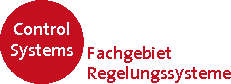
\includegraphics[width=1\textwidth]{Figures/csgLogo.pdf} 
%		\end{minipage}
%		\hfill
%		\begin{minipage}{0.12\textwidth}	
%		\end{minipage}
%		\hfill
%		% Logo Rechts
%		\begin{minipage}{0.23\textwidth}
%			\centering
%			\includegraphics[width=0.9\textwidth]{Figures/tu-logo.eps} %[width=1.47in]{Bilder/tu-logo.eps} 
%		\end{minipage}
%		%\hfill
%		% Fakultät und Institut rechts
%		\begin{minipage}{0.30\textwidth}
%			\large \Fakultaet \vspace{1.5mm}  \\ Institut f\"ur Energie- und  \\Automatisierungstechnik%\Institut
%		\end{minipage} %\Large
%	\end{minipage}
%	
%	% Zwischenraum
%	\vspace{4.5cm} %3cm
%	
%	% Haupt- und Untertitel 
%	{\Huge \Titel}\\[7mm]
%	\begin{minipage}{11cm}
%		\centering \LARGE   \flqq  \Untertitel \frqq
%	\end{minipage}\\
%	
%	% Zwischenraum
%	\vspace{1cm}%2.5cm
%	
%	% Gruppen- bzw. Autorenangabe
%	{\small \Gruppe}\\[0.2cm]
%	\begin{tabular}{rl}
%		\Autor  & \AutorMatrikelNr  \\
%		\ifdefempty{\AutorB}{}{\AutorB & \AutorBMatrikelNr \\} 
%		\ifdefempty{\AutorC}{}{\AutorC & \AutorCMatrikelNr \\} 
%		\ifdefempty{\AutorD}{}{\AutorD & \AutorDMatrikelNr \\} 
%		\ifdefempty{\AutorE}{}{\AutorE & \AutorEMatrikelNr \\} 
%	\end{tabular}
%	
%	% Zwischenraum
%	\vspace{3.3cm}%2cm
%	
%	% Grad
%	\begin{minipage}{11cm}
%		\centering
%		A thesis submitted for the degree of\\[0.3cm]
%		{\LARGE \textbf{-- Master of Science --}}\\[0.3cm]
%		in Computational Engineering Science
%	\end{minipage}
%	
%	
%	% 2.Zwischenraum
%	\vspace{3.3cm}
%	
%	% Professoren und Betreuer
%	\begin{tabular}{ll}
%		Examiner: & \Professor \\[1mm]
%		Co-Examiner: & \ProfessorII \\[1mm]
%		\ifdefempty{\BetreuerA}{}{Supervisor:  & \BetreuerA \\ }
%		\ifdefempty{\BetreuerB}{}{  & \BetreuerB \\ }
%	\end{tabular}
%	
%	% Umbruch bei langen Titeln verhindern
%	\enlargethispage{1cm}
%	
%	% Zwischenraum
%	\vfill
%	
%	% Footer erstellen
%	\Uni, \Fakultaet{} -- \Institut, \\ \Fachgebiet \\ \Datum
%	
%\end{titlepage}






%% !TEX encoding = UTF-8 Unicode
%% !TEX spellcheck = de_DE
%% !TEX root = ../main.tex
%
\begin{titlepage}
	\begin{spacing}{2}
			
			\begin{flushright} %rechtsbündig (Anfang)
					\vspace*{-20mm}
					\includegraphics[width=\textwidth]{Figures/title/CoverLogos.pdf}
					%\includegraphics[width=\textwidth]{skizzen/CoverLogos_MZH}
				\end{flushright} %rechtsbündig (Anfang)
			
			% der Titel der Arbeit:
			\vspace{38mm} {\centering {{\LARGE{\Titel}}} % Alternativ: Titel hier manuell eingeben und mit "\\"den Zeilenumbruch schön machen
					
					\vfill
					% hier kommt eine hübsche Grafik hin:
					\includegraphics[width = 80mm]{Figures/title/Robot_Assembly_3}
					
					
					\vfill }
		\end{spacing}
	\begin{spacing}{1}
			\begin{tabular}{l}
					\Large{\ArtDerArbeit~\Kennnummer}
					% Die einzutragende Nummer gibt es beim Betreuer!
				\end{tabular}
			
			\vspace{5mm}
			
			\begin{tabular}{l}
					\large{\Autor}\\
					\large{Matrikelnummer \AutorMatrikelNr}
				\end{tabular}
			
			\vspace{5mm}
			
			\begin{tabular}{l}
					\large{Hannover, \Datum}
				\end{tabular}
			
			
			\vspace{5mm}
			{\large
					\begin{tabular}{l l}						
							First Examiner  & \Erstpruefer\\
							Second Examiner & \Zweitpruefer\\
							Supervisor    	& \Betreuer\\
						\end{tabular}
				}
			
		\end{spacing}
\end{titlepage}
%\cleardoublepage

%include Declaration of Authorship
% !TEX encoding = UTF-8 Unicode
% !TEX spellcheck = de_DE
% !TEX root = ../main.tex

\newpage
% Logos oben einbinden
\begin{flushright}
			\vspace*{-20mm}
			\includegraphics[width=\textwidth]{Figures/title/CoverLogos.pdf}
\end{flushright}
	
\begingroup
\renewcommand{\cleardoublepage}{}
\renewcommand{\clearpage}{}
\chapter*{Declaration of Authorship}
\endgroup
\thispagestyle{empty}

%Kennnummer platzieren:
\begin{tikzpicture}[remember picture, overlay]
\node[xshift=-22mm,yshift=-43mm,anchor=north east,align=right] at (current page.north east){\Large{\textbf{\Kennnummer}}};
\end{tikzpicture}
%
%
\begin{tabular}{@{}p{0.25\textwidth} p{0.7\textwidth}}
\textbf{Name:} 		& \textbf{\Autor} \\ % Name des Autors
Registration no.: & \Matrikelnummer \\ % Matrikelnummer
\\
Thesis title: 		& \TitelDerArbeit \\
\\
Type of thesis: 	& \ArtDerArbeit\\
Study program: 		& Mechanical Engineering\\ % Please Choose:
Submission date:	& \Datum \\
\\
First examiner : 	& \Erstpruefer\\
Second examiner: 	& \Zweitpruefer\\
Supervisor: 			& \Betreuer
\end{tabular}

\vspace{10mm}

I, \emph{\Autor}, hereby affirm that the \ArtDerArbeit~entitled \emph{\TitelDerArbeit}~was written independently, that no references and aids other than those indicated were used, that all passages of the thesis which were taken over literally or analogously from other sources are marked as such and that the thesis has not yet been presented to any examination board in the same or similar form.

I hereby agree to the transmission of my work also to external services for plagiarism checking by plagiarism software.

\vspace{5mm}


\noindent Hannover, \Datum



\vspace{20mm}
(\Autor)

%\end{spacing}
% Leerseite einfügen
\cleardoublepage

% If desired, include a blank page
\input{FrontBackMatter/Leerseite}

% If desired, include a declaration of authorship
\chapter*{Eigenst\"andigkeitserkl\"arung}
\label{cha:Ehrenwort}
\thispagestyle{empty}
Hiermit erkl\"are ich, dass ich die vorliegende Arbeit selbstst\"andig und eigenh\"andig sowie ohne
unerlaubte fremde Hilfe und ausschlie\ss lich unter Verwendung der aufgef\"uhrten Quellen und
Hilfsmittel angefertigt habe.

\vspace{3cm}

\begin{tabular}{lp{4em}l}
 \hspace{4cm}   && \hspace{4cm} \\ \cline{1-1} \cline{3-3} \rule{0pt}{3.5ex} 
 Ort, Datum     && \Autor
\end{tabular}






% Include abstract

\selectlanguage{english}
\begin{abstract}
%General Problem
This thesis addresses the challenge of input trajectory transfer in heterogeneous multi-agent systems, where each agent has distinct system dynamics. \\
The concept of transfer learning has been applied to MAS to accelerate the learning process of a target agent by leveraging previously learned trajectories from a different source agent. However, directly transferring input trajectories between agents with dissimilar dynamics can lead to unwanted behaviour.
% Research Gap
This can be overcome by applying a mapping that transforms the input trajectory of the source system into an appropriate input trajectory for a target system so that their outputs match.
Obtaining such an input transfer map from simple experiments is difficult, so previous research often focuses on output transfer, adaptive control or strong similarity assumptions. Those approaches either require extensive model knowledge or have limited usability.  
 
% Content
%To address this problem, this thesis proposes a simple, data driven method to estimate a mapping used for input trajectory transfer.
This thesis provides a comprehensive understanding of trajectory transfer, distinguishing the input and output transfer cases and highlighting their similarities. Those insights are then used to propose a simple, data-driven method to estimate a dynamic input transfer map for SISO systems that addresses the aforementioned problem. Structural similarity in the systems is leveraged to simplify the estimation process further. The transfer map is estimated as a lifted system matrix and a transfer function. The performance of the estimated dynamic input transfer map is compared to a static map using a simple gain and to the direct transfer of the input trajectories.

% Contributions
It is shown that input and output transfer are equivalent under certain conditions. An input transfer map based on this assumption was able to significantly reduce the differences between a source and a target system in three simulated scenarios. This even includes scenarios where the systems have nonlinear, non-minimum phase dynamics. \\
Compared to a static map, the performance of a dynamic input transfer is superior, especially in cases where the estimated transfer map is applied to input trajectories which are not part of the training data. \\
Furthermore, the dynamic input transfer map can have a model order lower than the theoretically expected order of the transfer system, given that the source and target systems are related. Therefore, the expected order only provides an upper limit for the order of an estimated transfer map, and not a recommended choice. \\
Nonetheless, this thesis alone does not fully explore the potential and limitations of the proposed method. Future research is necessary to address these topics further.


%
%This can be leveraged to estimate an input transfer map from simple experiments. 
%
%This thesis therefore proposes an efficient data driven method to easily estimate a dynamic input transfer map from a simple training experiment. 
%
%For this, A differentiation between he input transfer case and the output transfer case is made and their similarities highlighted. 
%
%Previous methods make use of adaptive control or error prediction to overcome the challenge of dissimilar model dynamics. However
%Previous methods focus on adaptive control or error prediction overcome the challenge of dissimilar model dynamics,  restrictive similarity assumptions or require extensive model knowledge. This thesis addresses this problem by providing a data driven approch on input transfer estimation which leverages a less restrictive  
%
%- similar dynamics or model knowledge necessary
%- output transfer + static map
%- output transfe: easily estimated, this is not true for input transfer
%
%% this work does
%- trajectory transfer and concludes a correlation between input and output transfer
%- leverages structural similarity between agents to find an easy transfer map, which is less restictive than other sim assumptions
%- proposed method: 
%-- transfer function representation
%-- lifted system representation
%
%
%
%% contributions
%- input transfer vs output transfer
%- under certain conditions, input transfer and output transfer are identical
%- the transfer is dynamic system and not static, but can be ov much lower order the it would have been assumed
%
%
%The proposed method leverages structural similarity between two agents to estimate
%
%
%To overcome this challenge, several approaches have been proposed, including predicting the transfer's benefit, using adaptive controllers to force similar dynamics on all agents. A mapping between agents has been mostly studied for output trajectories.
%However, these approaches have limitations, such as disregarding potentially valuable source systems or requiring knowledge of the underlying dynamical systems.
%
%This thesis provides a more comprehensive understanding of input trajectory transfer. A differentiation between he input transfer case and the output transfer case is made and their similarities highlighted. 
%The insights were  In addition to this, the proposed method leverages structural similarity 
%
%expands current research through an efficient data-driven input transfer approach for learning control in unknown heterogeneous MAS. The proposed approach involves applying the same input sequence to different systems of a MAS, using the observed output sequences to learn the corresponding input transfer, and using the identified transfer to exchange information and improve the target agents learning performance.
%
%The thesis presents specific approaches to modeling and estimating input-transfer systems and evaluates the proposed methods in three simulated scenarios and a real-world system. The results show promising potential for the proposed approach in challenging MAS applications and highlight the importance of dynamic input transfer.

%Overall, this thesis provides a valuable contribution to the field of input trajectory transfer in MAS and proposes future research ideas in this area.\\
%%%
\par
\keywords{input transfer, trajectory transfer, transfer learning, multi-agent systems}
\end{abstract}





% If desired, uncomment the table of contents
\tableofcontents

% From the Backmatter --
% If desired, uncomment the list of figures
\listoffigures

% If desired, uncomment the list of tables
\listoftables

% If desired, uncomment the list of listings
%\lstlistoflistings

% Include this switch if symbols, abbreviations, etc., without reference in the document should be included in the directories (usually the case)
% \glsaddall
%\glsaddallunused

%\setglossarypreamble[main]{This list of glossary entries only includes the most important items. Descriptions might not be universal and are intended for this thesis.}

%% If desired, uncomment the glossary (will only be created if entries are available)
%\setglossarystyle{long3col}
%%\setglossarystyle{long}
%\renewenvironment{theglossary}%
% {\begin{longtable}{lp{\glsdescwidth}p{\glspagelistwidth}}}
	% %{\begin{longtable}[l]{lp{\glsdescwidth+\glspagelistwidth+0cm}}}%
		% {\end{longtable}}
	%\renewcommand{\glsnamefont}[1]{\textbf{#1}}
	%\printglossary[type=main, style=altlist]%[style=index]
	%\glsfindwidesttoplevelname
	%\glssetwidest[1]{transfer error dynamics}
	%\setglossarystyle{alttree}
	%\printglossary[type=main]
	
	% If desired, uncomment the abbreviations (will only be created if entries are available)
	%\printglossary[type=\acronymtype, nonumberlist]%[type=\acronymtype,style=list]
	
	% If desired, uncomment the symbols (will only be created if entries are available)
	%\printglossary[type=symbols, style=symb3spaltig, nonumberlist]
	%\printglossary[type=symbols, nonumberlist]
	
	%\chanumfalse
\addchap{Notation} % add chapter without numbering that appears in table of contents
% Manuelles Symbolverzeichnis
% ___________________________________________________________________
% ============================ NOTATION ==========================
% ====================================================================
\begin{table}[h]
	\renewcommand{\arraystretch}{1.4}
	\begin{tabularx}{1\textwidth}{@{}lX@{}}
		\toprule
		\textbf{Example} & \textbf{Description}  \\ \midrule
		$\mathbb{R}, \mathbb{N}$ 	& Capital letters in blackboard bold font represent common number types. \\
		$\mathcal{A}, \mathcal{T}$ 	& Capital letters in calligraphic font represent custom sets or its members. \\
		$\vec{A}, \vec{P}$ 			& Capital bold letters represent matrices.	\\
		$\vec{x}, \vec{f}$			& Lower-case bold letters represent column vectors or vector-functions. \\
		$F(z), T(s)$				& Capital regular letters represent transfer functions.	\\		
		$i, e^{(i \rightarrow j)}$	& Lower-case regular letters represent scalars and scalar-functions.\\
		$\vec{x}^{(i)}, F^{(2)}$	
			& A single upper, bracketed index represents the dependency on a single, specific agent.\\
		$ H^{(1, 2)}, e^{(i, j)}$ 
			& Two upper, bracketed indices represent the dependency on two specific agents, where the order of the agents is not relevant.\\
		$ H^{(1 \rightarrow 2)}, e^{(i \rightarrow j)}$
			& An arrow between two upper, bracketed indices represent the directional dependency on two specific agents, where the order of the agents matters.\\
		$\hat{\vec{t}}^{(i \rightarrow j)}, \hat{\mathbf{P}}^{(1)}$ 
	     	& An upper hat symbol represents an estimated or approximated entity.\\	
		$\bar H^{(1 \rightarrow 2)}, \bar e^{(i \rightarrow j)}$
	     	& An upper bar symbol represents a mean value.\\	
		\bottomrule
	\end{tabularx}
	\caption[General notation style]{General notation style. Some exceptions are possible.}
\end{table}

% ====================================================================
\begin{notebox}
	To be precise, the error dynamics depend on the order of agent $i$ and $j$, 
	since they differ in their sign.
		\begin{equation}
			H^{(i,j)}\neq H^{(j,i)}
		\end{equation}			
		However, both result in the same \gls*{output_error}. 
		$H^{(i,j)}$ and $H^{(j,i)}$ are not distinguished in this work, 
		which is consistent with the given notation. This also applies to other cases like the error trajectory $\vec{e}^{(i,j)}$ or the output error $\varepsilon^{(i,j)}_{\vec{u}}$ as well.
\end{notebox}

% ====================================================================
\pagebreak
\renewcommand{\arraystretch}{1.3}
\begin{tabularx}{1\textwidth}{@{}lX@{}}
    \endfirsthead \endhead \endfoot \endlastfoot
    \toprule
	\multicolumn{2}{@{}l}{\textbf{Mathematical Notations}} \\ 
	\textit{Symbol} & \textit{Description}  \\ \midrule
	$\left\Vert \cdot \right\Vert_2$ & denotes the 2-norm \\
	$\left\Vert \cdot \right\Vert_{\infty}$ & denotes the maximum-norm \\
	$ |\cdot |$	& 
	\begin{enumerate*}[label=(\roman*)]
		\item absolute of a number or 
		\item gain of a transfer function
	\end{enumerate*} \\
	$\angle $ & denotes the phase of a transfer function \\
	$\circ$	& denotes the composition of two functions or matrices \\
	$\vec{0}$ & denotes a zero vector or zero matrix  \\
	$\vec{I}$ & denotes the unit matrix \\
%		$\emptyset$ & denotes an empty set\\
	$\mathcal{N}(\mu, \sigma^2)$& normal distribution with mean $\mu$ and standard deviation $\sigma$ \\ 
	\bottomrule
	\multicolumn{2}{@{}l}{\textbf{General Parameters}} \\ 
	\textit{Symbol} & \textit{Description}  \\ \midrule
	$k, l$		 				&  running indeces \\
	$t$							&  time or duration (in seconds) \\
	$n_{\mathcal{A}}$	 		&  number of agents in a MAS \\
	$N, R$				 		&  dimension of a vector, matrix, i.e. length of an input trajectory \\
	$K$					 		&  degree of a biproper transfer function \\
	$K_N, K_D$		 	 		&	degree of numerator, denominator of a transfer function \\
	$m$						 	&  relative degree of a dynamic system \\
	$f_s, f_\mathrm{cutoff}, f$	&  sample frequency, cutoff frequency, other frequencies in $1/\unit{s}$\\ 
	\bottomrule
	\multicolumn{2}{@{}l}{\textbf{Sets \& Agents}} \\ 
	\textit{Symbol} & \textit{Description}  \\ \midrule
	$i, j$				 &  indices of a specific, but arbitrary agent in a MAS \\
	$\mathbb{R}$		 &	set of all real numbers \\
	$\mathbb{R}^n$		 &	$n$-dimensional set of all real numbers \\
	$\mathbb{N}_0$		 &  set of all natural numbers and zero \\
	$\mathcal{U}^{(i)}$	 	&  input space of agent $i$ \\
	$(\mathcal{U}^{(i)})^N$ &  input space of agent $i$ for input sequences of length $N$\\
	$(\mathcal{U}^{(i,j)})^N$&  input space of agent $i$ and $j$ for input sequences of length $N$ with 
	$(\mathcal{U}^{(i)})^N \cap (\mathcal{U}^{(j)})^N$ \\
    $\mathcal{A}$    	 &  set of all agents in a MAS\\
    $\mathcal{A}^{(i)}$  &  specific agent with index $i$\\
    $\mathcal{T}$    	 &  set of input maps between all agents in a MAS \\
    \bottomrule\\[10mm]\\[0.01mm]    
	\toprule
	\multicolumn{2}{@{}l}{\textbf{Discrete time step $k$}} \\ 
	\textit{Symbol} & \textit{Description}  \\ \midrule
	$k$			 &  time (sample) index for discrete systems and trajectories \\	    
    $u_{k}$		 & scalar input at time step $k$ \\
    $y_{k}$		 & scalar output at time step $k$ \\
   		$e^{(i,j)}_{k}$		 	 
   			& difference $y^{(j)}_k-y^{(j)}_k$ between the outputs of agent $i$ and $j$ at time $k$\\
   		$w_k$
   			& noise drawn from a normal distribution with zero mean and variance $\sigma^2$\\
    $\vec{x}^{(i)}_{k}$  & state of agent $i$ at time $k$ \\	
	$\vec{\tilde{f}}$ 	
		& state-function that advances the state $\vec{x}$ one step in time \\
	$\tilde{h}$ 	
		& output-function that returns the current output depending on the 
		current state and input\\   
	$\vec{A}, \vec{B}, \vec{C}$ 
		& state matrix, input matrix, output matrix of a linear system in discrete-time 
		state-space representation \\ \bottomrule
	\multicolumn{2}{@{}l}{\textbf{Transfer Function Representation}} \\ 
	\textit{Symbol} & \textit{Description}  \\ \midrule
	$s, z$ & denotes a transfer function in continuous time, discrete time\\
	$U(s), U(z)$		
		& System input in $s$-domain, $z$-domain\\
	$E(s), E(z)$		
		& $s$-Transformation, $z$-Transformation of the difference $y^{(j)}-y^{(j)}$\\
	$F$				
		& Transfer function of of a linear system\\
	$F^{(i\rightarrow j)}$	
		& \Glsc{deviation_system} in the transfer-function representation from agent $i$ to agent $j$	\\
	$Q$	
		& Filter function\\	
	$\hat{T}^{(i\rightarrow j)}$	
		& Estimation of the \glsc{input_map} in the transfer-function representation from agent $i$ to agent $j$\\
	$H^{(i,j)}$	
		& \Glsc{error_dynamics} in the transfer function representation describing the difference between agent 
		$i$ and $j$ when the same input is applied to both systems\\
	$H^{(i \rightarrow j)}$	
		& \Glsc{transfer_error_dynamics} in the transfer function representation describing the difference between agent 
		$i$ and $j$ including the input-transfer $\hat T^{(i \rightarrow j)}$\\	
	$a_k, b_k$ & Numerator, denominator coefficients in transfer-function \\ \bottomrule%\\[54mm]\\[0.01mm] \toprule
	\multicolumn{2}{@{}l}{\textbf{Batch Process \& Lifted System Representation}} \\ 
	\textit{Symbol} & \textit{Description}  \\ \midrule
	$\vec{u}, \vec{v}$		  	
		& An \glsc{input_trajectory} as a sequence of scalar inputs of length $N$\\
	$\vec{\tilde u}^{(i)}$	
		& Input trajectory of length $N$ for agent $i$ that results from some input-transfer 
		$\vec{t}^{(j\rightarrow i)}$\\
	$\vec{y}$		 	
		& An \glsc{output_trajectory} as a sequence of scalar outputs of length $N$\\
	$\vec{e}^{(i,j)}$
		& An \glsc{error_trajectory} describing the difference $\vec{y}^{(j)}-\vec{y}^{(i)}$ between the 
		output trajectories of agent $i$ and $j$\\
	$\vec{e}^{(i\rightarrow j)}_{\vec{u}}$
		& \Glsc{transfer_error_trajectory} describing the difference $\vec{y}^{(j)}-\vec{y}^{(i)}$ between the 
		output trajectories of agent $i$ and $j$ for a certain input trajectory $\vec{u}$\\ \midrule\\[0.1mm] \midrule
	\textit{Symbol} & \textit{Description}  \\ \midrule	
	$\vec{w}$
		& Sequence of normally distributed noise values with zero mean and variance $\sigma^2$\\ 	
	$\vec{f}$ 			
		& Nonlinear \glsc{batch_function} that maps a given input trajectory to a corresponding 
		output trajectory \\
	$\vec{f}^{(i\rightarrow j)}$
		& \Glsc{deviation_system} as a \gls*{batch_function} from agent $i$ to agent $j$\\
	$\mathbf{t}^{(i\rightarrow j)}$	
		& \Glsc{input_map} as a \gls*{batch_function} from agent $i$ to agent $j$\\
	$\mathbf{\hat t}^{(i\rightarrow j)}$	
		& Estimated input-transfer batch-function from agent $i$ to agent $j$
		(Here as a general expression for either $\mathbf{\hat T}^{(i\rightarrow j)}$ or $T^{(i\rightarrow j)}$)\\
	$\mathbf{h}^{(i\rightarrow j)}$	
		& \Glsc{error_dynamics} as a \gls*{batch_function} describing the difference between agent 
		$i$ and $j$ when the same input is applied to both systems.\\
	$\vec{P}$				
		& lifted-system matrix that maps an input trajectory to an output trajectory\\
	$\vec{P}^{(i\rightarrow j)}$	
		& \Glsc{deviation_system} in the lifted-system representation from agent $i$ to agent $j$\\
	$\mathbf{T}^{(i\rightarrow j)}$	
		& \Glsc{input_map} in the lifted-system representation from agent $i$ to agent $j$\\
	$p_k, p^{(i \rightarrow j)}_k$					
		& $k$-th parameter in lifted-system matrix $\vec{P}, \vec{P}^{(i\rightarrow j)}$\\
	$t^{(i\rightarrow j)}_k$	
		&  $k$-th parameter in lifted-system matrix $\mathbf{T}^{(i\rightarrow j)}$\\ \bottomrule
	\multicolumn{2}{@{}l}{\textbf{Error Metrics}} \\ 
	\textit{Symbol} & \textit{Description}  \\ \midrule
   		$\varepsilon^{(i,j)}$ % \left(\vec{y}^{(i)}, \vec{y}^{(j)}\right)	 	 
   			& \Glsc{output_error}: 2-norm of the difference between the output trajectories of agent $i$ and $j$\\	
   		$\varepsilon^{(i,j)}_{\vec{u}}$ %\left(\vec{u}^{(i)}\right)		 	 
   			& \Glsc{direct_transfer_error}: Output error $e^{(i,j)}$ when the same input is applied 
   			to agents $i$ and $j$ \\
	$\varepsilon^{(i\rightarrow j)}_{\vec{u}}$ 
		& \Glsc{transfer_error}: Output error $\varepsilon^{(i,j)}$  for a certain input trajectory $\vec{u}$ 
			after applying the \gls*{input_map} $\vec{t}^{(i \rightarrow j)}$ to agent $j$ \\	
	$\varepsilon^{(i\rightarrow j)}_{\vec{u},\mathrm{NRMS}}$ 
		& \Glsc{nte}: Transfer error $\varepsilon^{(i\rightarrow j)}_{\vec{u}}$ 
		normalized to the \gls*{direct_transfer_error} $\varepsilon^{(i,j)}_{\vec{u}}$\\	
	\bottomrule
	\caption{Mathematical notations}
\end{tabularx}

\chanumtrue
    
	% --
	
	% Save page number for Back Matter and conclude Front Matter
\newcounter{RomanNumbers}
\addtocounter{RomanNumbers}{\value{page}}
\clearpage

%
%% Body Matter - Here the text of the document, the content, is set
% Page numbers of the content in Arabic numerals
\pagenumbering{arabic}

% Content

% Inserting the files, e.g.:
%\chapter{Introduction}

\graphicspath{{./Figures/Introduction/}}



\section{Motivation}
%This section should explore the underlying reasons for undertaking the research. It might include the importance of the topic, the gap in current knowledge, and the potential applications of the research findings.
%figure for Handle Boston Dynamics Robot
\begin {figure}[h]
\centering
\includegraphics[width=0.7\textwidth]{boston-dynamics-handle-robot}
\caption{Handle Robot by Boston Dynamics\cite{handle}}
\label{fig:Handle}
\end {figure}


Robotics has always been a cutting-edge field that combines sophisticated engineering, artificial intelligence, and a comprehension of human-environment interactions.
This study is motivated by multiple important elements, all of which highlight the importance and relevance of the research.
This research is motivated by the aim to contribute to the development of robotics, address some of the current knowledge gaps in the field, and foster interdisciplinary collaboration.
This research aims to contribute to the field of robotics by developing a multi-legged robotic system.
The focus is on improving movement capabilities and control strategies, with the hope of offering valuable insights into robotic design and functionality.
Even with significant advancements, there are still many unanswered questions about robotic control and locomotion, particularly in systems that replicate biological structures and processes.
Complex dynamic tasks that living beings handle with ease are sometimes difficult for traditional robotic systems to accomplish. This research aims to close these gaps by concentrating on a multi-legged robot that finds inspiration in the natural environment. This will provide insights into more realistic and effective movement tactics. The applications of such advanced robotic systems are vast and varied, ranging from search and rescue operations in hazardous environments to assistive technology in warehouse automation.By pushing the boundaries of what is currently possible in robotic design and control, this research has the potential to make contributions to fields where human intervention is limited, dangerous, or impractical. This project is inherently interdisciplinary, integrating concepts from mechanical engineering, computer science, control theory, and even biology. Such cross-disciplinary collaboration is crucial for driving innovation, as it allows for the exchange of ideas and methods from diverse fields. This approach is expected to yield novel solutions and advancements that could extend well beyond the scope of this project.

%\textbf{Advancements in Robotic Technologies:}% Robotics has grown at an exponential rate over the past few decades, resulting in improved capabilities and more applications. Previously limited to industrial settings, robots are now being deployed in increasingly dynamic and unpredictable circumstances. The development of robotic systems that are more flexible, nimble, and intelligent is required due to this evolution. Our research is to create a sophisticated multi-legged robotic system that can perform intricate movements and interact with its surroundings.

%\textbf{Filling Knowledge Gaps:} %Even with significant advancements, there are still many unanswered questions about robotic control and locomotion, particularly in systems that replicate biological structures and processes. Complex dynamic tasks that living beings handle with ease are sometimes difficult for traditional robotic systems to accomplish. This research aims to close these gaps by concentrating on a multi-legged robot that finds inspiration in the natural environment. This will provide insights into more realistic and effective movement tactics.

%\textbf{Potential for Broad Impact:} %The applications of such advanced robotic systems are vast and varied, ranging from search and rescue operations in hazardous environments to assistive technology in healthcare. By pushing the boundaries of what is currently possible in robotic design and control, this research has the potential to make significant contributions to fields where human intervention is limited, dangerous, or impractical.

%\textbf{Interdisciplinary Collaboration and Innovation:} %This project is inherently interdisciplinary, integrating concepts from mechanical engineering, computer science, control theory, and even biology. Such cross-disciplinary collaboration is crucial for driving innovation, as it allows for the exchange of ideas and methods from diverse fields. This approach is expected to yield novel solutions and advancements that could extend well beyond the scope of this project.

%In summary, the motivation for this project lies in its potential to advance the field of robotics, fill existing knowledge gaps, have a broad societal impact, and foster interdisciplinary collaboration. By developing a multi-legged robotic system with enhanced movement capabilities and control strategies, this research endeavors to set new standards in robotic design and functionality.

\section{Explanation of the Goals and Requirements}
In this research, we aim to develop a multi-legged robotic system that can perform complex movements and interact with its environment.
The robot will be able to balance on two wheeled multi-jointed legs.
The robot would be based on the previous TWIPR robot.
Extra degrees of freedom will be added to the robot to allow for more complex movement.
Compact and lightweight components will be used.
The new robot will be bigger than the previous one but still small enough to be easily transported and work with it in a small space.
The robot would be designed from scratch to meet the requirements of the project.
The robot would be designed using CAD software.
The design would take into account the mechanical, electrical, and software requirements of the robot.
Fabrication of the robot chassis would be done using 3D printing.
Electrical design and assembly would be done using off-the-shelf components.
Mathematical modeling and simulation of the robot would be done to determine the robot's dynamics and control.
Different control strategies would be explored and implemented.
Development of firmware and software for the robot would be done.
The robot would be tested and evaluated in simulation and in real life.
The robot would be tested for its ability to balance and move in different environments.
The robot would be tested for its ability to perform complex movements and interact with its environment.
For the exploration of experimental methods and different learning algorithms, we need cheap to build and easily be repaired robot.
%\include{Content/Chapter1}
%\include{Content/Conclusion}

% Then insert chapters in the files.
% % % % % % % % % % % % % % % % % % % % % % % % % % % % % % % % % % % % % % % % % % % % % % %
\chapter{Introduction}

\graphicspath{{./Figures/Introduction/}}



\section{Motivation}
%This section should explore the underlying reasons for undertaking the research. It might include the importance of the topic, the gap in current knowledge, and the potential applications of the research findings.
%figure for Handle Boston Dynamics Robot
\begin {figure}[h]
\centering
\includegraphics[width=0.7\textwidth]{boston-dynamics-handle-robot}
\caption{Handle Robot by Boston Dynamics\cite{handle}}
\label{fig:Handle}
\end {figure}


Robotics has always been a cutting-edge field that combines sophisticated engineering, artificial intelligence, and a comprehension of human-environment interactions.
This study is motivated by multiple important elements, all of which highlight the importance and relevance of the research.
This research is motivated by the aim to contribute to the development of robotics, address some of the current knowledge gaps in the field, and foster interdisciplinary collaboration.
This research aims to contribute to the field of robotics by developing a multi-legged robotic system.
The focus is on improving movement capabilities and control strategies, with the hope of offering valuable insights into robotic design and functionality.
Even with significant advancements, there are still many unanswered questions about robotic control and locomotion, particularly in systems that replicate biological structures and processes.
Complex dynamic tasks that living beings handle with ease are sometimes difficult for traditional robotic systems to accomplish. This research aims to close these gaps by concentrating on a multi-legged robot that finds inspiration in the natural environment. This will provide insights into more realistic and effective movement tactics. The applications of such advanced robotic systems are vast and varied, ranging from search and rescue operations in hazardous environments to assistive technology in warehouse automation.By pushing the boundaries of what is currently possible in robotic design and control, this research has the potential to make contributions to fields where human intervention is limited, dangerous, or impractical. This project is inherently interdisciplinary, integrating concepts from mechanical engineering, computer science, control theory, and even biology. Such cross-disciplinary collaboration is crucial for driving innovation, as it allows for the exchange of ideas and methods from diverse fields. This approach is expected to yield novel solutions and advancements that could extend well beyond the scope of this project.

%\textbf{Advancements in Robotic Technologies:}% Robotics has grown at an exponential rate over the past few decades, resulting in improved capabilities and more applications. Previously limited to industrial settings, robots are now being deployed in increasingly dynamic and unpredictable circumstances. The development of robotic systems that are more flexible, nimble, and intelligent is required due to this evolution. Our research is to create a sophisticated multi-legged robotic system that can perform intricate movements and interact with its surroundings.

%\textbf{Filling Knowledge Gaps:} %Even with significant advancements, there are still many unanswered questions about robotic control and locomotion, particularly in systems that replicate biological structures and processes. Complex dynamic tasks that living beings handle with ease are sometimes difficult for traditional robotic systems to accomplish. This research aims to close these gaps by concentrating on a multi-legged robot that finds inspiration in the natural environment. This will provide insights into more realistic and effective movement tactics.

%\textbf{Potential for Broad Impact:} %The applications of such advanced robotic systems are vast and varied, ranging from search and rescue operations in hazardous environments to assistive technology in healthcare. By pushing the boundaries of what is currently possible in robotic design and control, this research has the potential to make significant contributions to fields where human intervention is limited, dangerous, or impractical.

%\textbf{Interdisciplinary Collaboration and Innovation:} %This project is inherently interdisciplinary, integrating concepts from mechanical engineering, computer science, control theory, and even biology. Such cross-disciplinary collaboration is crucial for driving innovation, as it allows for the exchange of ideas and methods from diverse fields. This approach is expected to yield novel solutions and advancements that could extend well beyond the scope of this project.

%In summary, the motivation for this project lies in its potential to advance the field of robotics, fill existing knowledge gaps, have a broad societal impact, and foster interdisciplinary collaboration. By developing a multi-legged robotic system with enhanced movement capabilities and control strategies, this research endeavors to set new standards in robotic design and functionality.

\section{Explanation of the Goals and Requirements}
In this research, we aim to develop a multi-legged robotic system that can perform complex movements and interact with its environment.
The robot will be able to balance on two wheeled multi-jointed legs.
The robot would be based on the previous TWIPR robot.
Extra degrees of freedom will be added to the robot to allow for more complex movement.
Compact and lightweight components will be used.
The new robot will be bigger than the previous one but still small enough to be easily transported and work with it in a small space.
The robot would be designed from scratch to meet the requirements of the project.
The robot would be designed using CAD software.
The design would take into account the mechanical, electrical, and software requirements of the robot.
Fabrication of the robot chassis would be done using 3D printing.
Electrical design and assembly would be done using off-the-shelf components.
Mathematical modeling and simulation of the robot would be done to determine the robot's dynamics and control.
Different control strategies would be explored and implemented.
Development of firmware and software for the robot would be done.
The robot would be tested and evaluated in simulation and in real life.
The robot would be tested for its ability to balance and move in different environments.
The robot would be tested for its ability to perform complex movements and interact with its environment.
For the exploration of experimental methods and different learning algorithms, we need cheap to build and easily be repaired robot.
\chapter{Literature Review}

\graphicspath{{./Figures/Literature Review/}}


\section{Overview of Two-Wheeled Inverted Pendulum Robots (TWIPR)}

%figure for Ascento robot
\begin {figure}[h]
\centering
\includegraphics[width=0.5\textwidth]{Ascento robot}
\caption{Ascento Robot by ETH Zurich\cite{klemm2019ascento}}
\label{fig:Ascento robot}
\end {figure}

The Legged Two-Wheeled Inverted Pendulum Robot (LTWIPR) is a type of mobile robot that has two wheels and a body carried by two legs.
The robot acts as an inverted pendulum, with the wheels acting as the pivot point.
The robot is able to balance itself on the two wheels. The robot is able to move by tilting the body forward or backward, causing the wheels to rotate in the direction of the tilt. The robot is able to turn by moving the wheels in opposite directions. The robot is able to move in any direction by combining these movements. LTWIPRs are able to move in a variety of environments, including rough terrain and stairs. LTWIPRs are able to perform complex movements, such as jumping and climbing. LTWIPRs are able to interact with their environment, such as navigating around obstacles and diving under obstacles.



\section{Prior Works and Advances in Multi-Legged Robotic Systems}
%This section should provide a comprehensive review of existing literature relevant to your research topic. It should cover key theories, models, experiments, and findings in the field, particularly focusing on works that directly relate to your research question or hypothesis. This review not only shows your understanding of the field but also how your work fits into and contributes to the existing body of knowledge.
\subsection{Mechanical Design and Development of Wheeled Robots}

\subsection{Dynamic Modeling of Wheeled Bipedal Robots}
\subsection{Control of Wheeled Bipedal Robots}
\subsection{Integration of Learning and Adaptive Control Mechanisms in Wheeled Bipedal Robots}
\subsection{Applications and Future Directions}


\chapter{Mechanical Design}

\graphicspath{{./Figures/Mechanical Design/}}
%	\item Outline the purpose and scope of the chapter.
 Modeling In this chapter, the details of the mechanical design are presented.
 where it goes from the initial conceptual design to the final design showing in the process the design decision-making for each critical point, This chapter emphasis the detailed description of the precise placement and alignment of different components such as the motors, wheels, battery, boards, and others to maintain the seamless integration of all the components into the robot body.
%	\item Briefly describe the mechanical design's role in the overall project.
\newline
The mechanical design serves as an important pillar to define the new physical form, size, and shape of the TWIPR. Depending on how these criteria are defined, the robot would interact with the environment.
taking into account that the design directly influences the center of gravity, which is crucial to consider in our robot due to the inverted pendulum nature to be able to balance and maintain the upright position.
In addition to the impact that the design has on the maneuverability of the robot and how it would respond to the control signals to be able to execute a task.
\newpage
\section{Design Objectives and Requirements}

%	Detail the primary objectives of the mechanical design
	The main objective is to come up with a new design for a multiple joints Robot to perform complex dynamic movements.
	This robot would be based on the Two wheeled inverted pendulum robots.
	The new design would add more degrees of freedom to enable the more complex movements.
	This enhances the robot's capabilities where it can execute more diverse scenarios.
%	\item List the requirements that the design must meet (e.g., weight limits, size constraints, mobility requirements).
	Initially, the main requirement was to add two more degrees of freedom where originally it used to have one degree of freedom in the wheels.
	The new design has three degrees of freedom, one in the wheels, one as a knee joint and one as a hip joint.
	The current design has two identical legs.

\section{Conceptual Design}
%Discuss the initial design concepts.
As for the initial design concepts the body was that main point of focus as shown in the figure \ref{fig:initialdesigns}.Three initial designs where considered mainly for the body.\ Symmetrical vertical body in figure A, symmetrical horizontal body in figure B and leaning forward body in figure C\@.
\ For the three designs, two independent legs where considered.
two designs where considered for the legs, the normal joint leg and the compliant leg

\begin{figure}[h]
	\centering
	\includegraphics[width=1\linewidth]{Conceptual Design}
	%\includegraphics[width=0.5\linewidth]{Figures/Mechanical Design/Conceptual_Design}
	\caption[Initial Design Concepts]{Three initial Design Concepts for the robot body}
	\label{fig:initialdesigns}
\end{figure}
Two main designs where considered for the legs as shown in the figure \ref{fig:legdesignsjbhi}, the normal joint leg and the compliant leg.
The compliant leg is more flexible and can be used to absorb the shock from the ground.\ The normal joint leg is more rigid and can be used to generate more torque.in addition, the normal is more relative to our use-case as it can precisely control the position of the leg.
% figure for the leg designs concepts
\begin{figure}[h]
	\centering
	\includegraphics[width=0.4\linewidth]{Leg Design}
	\caption[Leg Design Concepts]{Leg Design Concepts}
	\label{fig:legdesignsjbhi}
\end{figure}

%Explain the decision-making process for selecting the final concept.
% Include sketches or early design models.
\section{Schmatic Representation of the Robot}
% the schematic representation of the robot should show the location of the different components such as the motors, wheels, battery, boards, and others
%figure for the schematic representation of the robot
\subsection{Schmatic overview of the robot}
%figure for the schmatic overview of the robot
\begin{figure}[h]
	\centering
	\includegraphics[width=0.5\linewidth]{schmatic overview of the robot}
	\caption[schmatic overview of the robot]{schmatic overview of the robot}
	\label{fig:schmaticoverviewoftherobot}
\end{figure}
As shown in the figure \ref{fig:schmaticoverviewoftherobot}, In order to achieve the desired movements using the new articulated legs, then we need three motors on each leg, one motor for the wheel, one motor for the knee joint and one motor for the hip joint.
In addition to the motors, the robot needs a battery to power the motors, a control board to control the motors, and a power management board to manage the power distribution between the different components. Some of the components  are passed on from the previous TWIPR robot such as the control board, the power management board. For more information about the electronic components and there specifications, please refer to the electronics design chapter.

\section{Initial Calculations}
%figure for the initial calculations
\begin{figure}[h]
	\centering
	\includegraphics[width=0.7\linewidth]{Initial Calculations}
	\caption[Initial Calculations]{Initial Calculations}
	\label{fig:initialcalculations}
\end{figure}
One of the main critical positions for the robot, as shown in the figure \ref{fig:initialcalculations} is the position where the center of mass of the body and the center of mass of the legs are the furthest away from point x on the horizontal axis.It is important to make the initial torque calculations to be able to select the right motors for the robot.
Starting from that position first, the robot should be able to balance itself and maintain the upright position.
secondly, the robot should be able to change the knee angle to lift the body while maintaining its balance.
The calculations are based on some assumptions and simplifications, Considering only half the body weight and one leg.
As shown in the figure, The Wheel motor shaft is aligned with the hip joint, the minimum torque required to balance the robot is calculated as follows:

The summation of the torques around point x should be equal to zero to maintain the balance with minimum motor torque.
\begin{equation}
	\sum_{i=1}^{n} \tau_{i}=0
\end{equation}
\begin{equation}
	\sum_{i=1}^{n} \tau_{i}=m_{B}gI-m_{K}g(0.7)D
\end{equation}
\begin{equation}
	\sum_{i=1}^{n} \tau_{i}=0.704(9.81)(0.03)-0.2(9.81)(0.7)(0.15)\approx0 \mathrm{Nm}
\end{equation}
The Lengths of D and I can be modified to make sure that the summation of the torques around point x is equal or approximately equal to zero.
This will make sure that the robot can balance itself with minimum wheel motor torque.
The torques can cancel each other out by readjusting the lengths of D or I and also by modeling the weight distribution in the body and the legs.

The torque required to lift the body is calculated around the knee joint point y as follows:
\begin{equation}
	\sum_{i=1}^{n} \tau_{i}=m_{B}g(D+I)-m_{K}g(0.3)D
\end{equation}
\begin{equation}
	\sum_{i=1}^{n} \tau_{i}=0.704(9.81)(0.03+0.15)-0.2(9.81)(0.3)(0.15) \approx 1.154 \mathrm{Nm}
\end{equation}
1.154 $\mathrm{Nm}$ is the minimum torque required to hold the body in position.
The Knee motor should be able to generate more torque to be able to lift the body and change the knee angle.

The approximate masses of the body and the legs are estimated in the table\ref{tab:initialcalculationsassumptions}.
After manufacturing the parts and assembling the robot, the actual masses of the body and the legs are measured and the calculations are updated accordingly.
\begin{table}[h]
	\centering
	\caption{Initial Calculations Assumptions}
	\label{tab:initialcalculationsassumptions}
	\begin{tabular}{lcl}
		\toprule
		Parameter & Value & Description 			  \\
		\midrule
		$m_B$         & 0.704 kg  & Mass of the body  \\
		$m_K$         & 0.2 kg  & Mass of the Knee including the two legs\\
		$L_1$         & 0.15 m   & Length of Link 1  \\
		$L_2$         & 0.15 m   & Length of Link 2   \\
		$D$ 	  	  & 0.03 m   & distance from the Wheel axis to the center of mass of leg \\
		$I$ 	  	  & 0.03 m   & distance from the hip joint axis to the center of mass of the body   \\
		\bottomrule
	\end{tabular}
\end{table}

\begin{notebox}
	\textbf{To reduce the needed torque to lift we can:}
	%bullit points
	\begin{itemize}
		\item Shorten the links
		\item Reduce the body weight
		\item Use gearbox to increase the torque
	\end{itemize}
\end{notebox}
%To reduce the needed torque to lift the body, we can:
%\begin{itemize}
%	\item Shorten the links
%	\item Reduce the body weight
%	\item Use gearbox to increase the torque
%\end{itemize}

\newpage
\section{Detailed Design Development}
% Elaborate on the development of the detailed mechanical design.
Throughout the design process, modularity and ease of assembly were considered.
The design was broken down into three main parts: the body, the hip-knee link, and the knee-wheel link.
Print iterations were made to ensure that the parts fit together and that the robot could be assembled with ease. Modifications were made to simplify the printing process and reduce the support material used.


\subsection{Body Design}
% Discuss the design of the body.
The body design is the main part of the robot, it is the main structure that holds all the components together.
The components that are mounted on the body are the hip motors, the battery, camera, sensor, a rack that includes the power distribution board, the microcontroller board attached to the Raspberry Pi. The optimization of the body design is crucial to be able to fit all the components in a compact form and at the same time distribute the weight equally to maintain the balance of the robot.
Different design features were considered, such as the cable management, the fastening features specifically designed to easily mount the battery, organizing the cable between the boards and the rest of the robot parts.
Opening slots were to one side of the body to be able to access the boards and connect charging cables to the battery.
%figure 1 for the body design
\begin{figure}[h]
	\centering
	\includegraphics[width=1\linewidth]{Body_Design_1}
	\caption[TOP view of the Body Design]{TOP view of the Body Design}
	\label{fig:bodydesign1}
\end{figure}
%figure 2 for the body design
\begin{figure}[h]
	\centering
	\includegraphics[width=1\linewidth]{Body_Design_2}
	\caption[Side view of the Body Design]{side view of the Body Design}
	\label{fig:bodydesign2}
\end{figure}
\vspace{10cm}
%figure 3 for the body design
\begin{figure}[h]
	\centering
	\includegraphics[width=0.8\linewidth]{Body_Design_3}
	\caption[3D view of the Body Design]{3D view of the Body Design}
	\label{fig:bodydesign3}
\end{figure}

\newpage
\subsection{Hip Knee Link Design}
% Discuss the design of the hip knee Link.
This link connects the hip body axis to the knee axis.
The design of this link includes the knee motor housing form one-side and a frame to attach to the output horn of the hip motor.
The motor housing is designed to ensure the fixed placement of the motor inside the link, As shown in the figure, \ref{fig:bodykneelink1} Cable management is also considered in the design of this link to make sure that the cables are not interfering with the movement of the link.The curvature of the link creates enough clearance so that when the hip axis is aligned with the wheel axis, they would not touch with each other even when considering the elastic bending of the legs.
%figure 1 for the Body_Knee_link
\begin{figure}[h]
	\centering
	\includegraphics[width=1\linewidth]{Body_Knee_Link_1}
	\caption[TOP view of the Body Knee Link]{TOP view of the Body Knee Link}
	\label{fig:bodykneelink1}
\end{figure}
%figure 2 for the Body_Knee_link
\begin{figure}[h]
	\centering
	\includegraphics[width=1\linewidth]{Body_Knee_Link_2}
	\caption[Side view of the Body Knee Link]{side view of the Body Knee Link}
	\label{fig:bodykneelink2}
\end{figure}
%figure 3 for the Body_Knee_link
\begin{figure}[h]
	\centering
	\includegraphics[width=1\linewidth]{Body_Knee_Link_3}
	\caption[3D view of the Body Knee Link]{3D view of the Body Knee Link}
	\label{fig:bodykneelink3}
\end{figure}

\newpage
\subsection{Knee Wheel Link Design}
% Discuss the design of the Wheel_Knee_link.
This link connects the knee axis to the wheel axis.
The design of this link includes the wheel motor mounting form one-side and a frame to attach to the output horn of the knee motor from the other side. The motor mounting is designed to ensure the fixed placement of the motor on the link, As shown in the figure, \ref{fig:wheelkneelink2}. Cable management is also considered in the design of this link by adding a cable fastener and holes to pass the cables through the link.
%figure 1 for the Wheel_Knee_link
\begin{figure}[h]
	\centering
	\includegraphics[width=1\linewidth]{Wheel_Knee_Link_1}
	\caption[SIDE view of the Knee Wheel Link]{SIDE view of the Knee Wheel Link}
	\label{fig:wheelkneelink1}
\end{figure}
%figure 2 for the Wheel_Knee_link
\begin{figure}[h]
	\centering
	\includegraphics[width=1\linewidth]{Wheel_Knee_Link_2}
	\caption[TOP view of the Knee Wheel Link]{TOP view of the Knee Wheel Link}
	\label{fig:wheelkneelink2}
\end{figure}
%figure 3 for the Wheel_Knee_link
\begin{figure}[h]
	\centering
	\includegraphics[width=1\linewidth]{Wheel_Knee_Link_3}
	\caption[3D view of the Knee Wheel Link]{3D view of the Knee Wheel Link}
	\label{fig:wheelkneelink3}
\end{figure}


\newpage
\subsection{Boards Mounting rack}
% Discuss the design of the Boards Mounting rack.
As shown in the figure \ref{fig:pcbrack1},\ref{fig:pcbrack2},\ref{fig:pcbrack3}, the board mounting rack is designed to hold the power distribution board, the microcontroller board, and the Raspberry Pi.
The rack is designed to be mounted in the body of the robot by using four screws.
Appropriate space is considered between the two boards as well as the clearance between the rack and the battery underneath it and the body cover on top of it.
%figure 1 for the PCB_Rack
\begin{figure}[h]
	\centering
	\includegraphics[width=.7\linewidth]{PCB_Rack_1}
	\caption[Side view of the PCB Rack]{Side view of the PCB Rack}
	\label{fig:pcbrack1}
\end{figure}
%figure 2 for the PCB_Rack
\begin{figure}[h]
	\centering
	\includegraphics[width=.7\linewidth]{PCB_Rack_2}
	\caption[Top view of the PCB Rack]{Top view of the PCB Rack}
	\label{fig:pcbrack2}
\end{figure}
%figure 3 for the PCB_Rack
\begin{figure}[h]
	\centering
	\includegraphics[width=.7\linewidth]{PCB_Rack_3}
	\caption[3D view of the PCB Rack]{3D view of the PCB Rack}
	\label{fig:pcbrack3}
\end{figure}
\newpage
\subsection{Motor Cover}
% Discuss the design of the Motor Cover.
The motor cover is designed to protect the motor from any external objects that might interfere with the motor operation.
The motor cover is designed to be mounted on the wheel knee link with the consideration of the clearance between the motor cover and hip knee link.
Slots are designed to dissipate the heat generated from the motor as shown in the figure \ref{fig:motorcover1}, \ref{fig:motorcover3}.
%fugure 1 for the motor_cover
\begin{figure}[h]
	\centering
	\includegraphics[width=.6\linewidth]{motor_cover_1}
	\caption[Side view of the Motor Cover]{Side view of the Motor Cover}
	\label{fig:motorcover1}
\end{figure}
%fugure 2 for the motor_cover
\begin{figure}[h]
	\centering
	\includegraphics[width=.6\linewidth]{motor_cover_2}
	\caption[Top view of the Motor Cover]{Top view of the Motor Cover}
	\label{fig:motorcover2}
\end{figure}
%fugure 3 for the motor_cover
\begin{figure}[h]
	\centering
	\includegraphics[width=.6\linewidth]{motor_cover_3}
	\caption[3D view of the Motor Cover]{3D view of the Motor Cover}
	\label{fig:motorcover3}
\end{figure}


\newpage
\subsection{Full Design}


%figure 1 for the Robot_Assembly
\begin{figure}[h]
	\centering
	\includegraphics[width=.6\linewidth]{Robot_Assembly_1}
	\caption[Side view of the Robot Assembly]{Side view of the Robot Assembly}
	\label{fig:robotassembly1}
\end{figure}
%figure 2 for the Robot_Assembly
\begin{figure}[h]
	\centering
	\includegraphics[width=.6\linewidth]{Robot_Assembly_2}
	\caption[Top view of the Robot Assembly]{Top view of the Robot Assembly}
	\label{fig:robotassembly2}
\end{figure}
%figure 3 for the Robot_Assembly
\begin{figure}[h]
	\centering
	\includegraphics[width=1\linewidth]{Robot_Assembly_3}
	\caption[3D view of the Robot Assembly]{3D view of the Robot Assembly}
	\label{fig:robotassembly3}
\end{figure}
\vspace{3cm}
The full design of the robot is shown in the figure\ref{fig:robotassembly3}.
The robot is designed to be assembled in a modular way.
The full assembly reveals how all the parts fit together.
This includes the body, the hip-knees, the knee-wheel links, the motor cover, the boards mounting rack,the hip motors, the knee motors, the camera, the sensor, the face shield, the body cover,the BaneBots shaft hub, and the wheels.
After assembling the robot, different movements configurations are tested using the CAD software to make sure that the robot can move freely without any interference between the different parts.
\newpage
%sub section for the dimentions of the robot
\subsection{Dimensions}
%figure for the dimensions of the robot
As shown in the figure \ref{fig:robotassemblyv2side}, \ref{fig:robotassemblyv2top}, the main dimensions of the robot are shown.
Comparing the dimensions of the robot to the dimensions of the previous TWIPR robot, the new robot is much bigger in size because of the addition of the two legs.
Compactness was not a main concern in the design of the robot, the main concern was to make sure that the robot can perform the required movements and interact with the environment.
\begin{figure}[h]
	\centering
	\includegraphics[width=0.5\linewidth]{Robot_Assembly_V2_Side}
	\caption[Side view of the Robot Assembly]{Side view of the Robot Assembly}
	\label{fig:robotassemblyv2side}
\end{figure}
%figure for the dimensions of the robot top view
\begin{figure}[h]
	\centering
	\includegraphics[width=0.5\linewidth]{Robot_Assembly_V2_Top}
	\caption[Top view of the Robot Assembly]{Top view of the Robot Assembly}
	\label{fig:robotassemblyv2top}
\end{figure}
\newpage
\subsection{Safety considerations}
% the motor cover, the face shield of the body and the body cover
Safety is a crucial aspect to consider in the design of the robot.
The robot is designed to be safe to operate in the environment and safe to interact with humans.
Clearances are considered in the design to make sure that moving parts wouldn't interfere with each other.
The motor cover is designed to protect the motor from any external objects that might interfere with the motor operation.
%Two subfigures side by side of the motor cover
%two subfigures side by side of the face shield
\begin{figure}[h]
	\centering
	\begin{subfigure}[b]{0.4\textwidth}
		\centering
		\includegraphics[width=.5\linewidth]{Support_flexible_1}
		\caption{Face Shield Side View}
		\label{fig:face shield side view}
	\end{subfigure}
	\hfill
	\begin{subfigure}[b]{0.4\textwidth}
		\centering
		\includegraphics[width=.5\linewidth]{Support_flexible_2}
		\caption{Face Shield 3D View}
		\label{fig:faseshield3dview}
	\end{subfigure}
	\caption{Face Shield}
	\label{fig:faceshield}
\end{figure}

The face shield of the body is designed to protect the components inside the body.
The face shield is designed to be flexible to absorb the shock from any external objects that might hit the robot. It is screwed with two screws to the body.
%cable mangment
The cable management is considered in the design of the robot to make sure that the cables are routed from and to all the components in the robot in a safe way to protect the cables form tearing or getting damaged as well as to protect the cables from interfering with the movement of the robot.



\section{Design for Manufacturability and Assembly}
% Discuss how the design facilitates manufacturing and assembly.
% Explain any design choices made to simplify these processes of manufacturing and assembly.
% Discuss any design features that were added to facilitate the manufacturing and assembly processes.
Design for manufacturability and assembly was considered throughout the design process.
Design consideration was taken into account to make sure that the robot parts can be printed using 3D printing technology.
Considering the limitations of 3D printing technology, the design was modified to make sure that the parts can be printed with acceptable quality.
The orientation at which the parts are printed was considered while designing the parts.
Assembly fitting and clearance were considered to make sure that the parts can be assembled with ease.

\section{Prototyping and Iterative Design}
% Discuss the process of prototyping.
% Explain how feedback from prototyping phases was incorporated into design revisions.

During the design process, the sketches for the different parts were drawn relying on each other so that future modifications can be easily applied.
 The design was prototyped using 3D printing.
Therefore, different problems were encountered during the prototyping process.
The problems were analyzed and the design was modified accordingly to solve the problems.
Some of the problems were related to the 3D printing process, and some were related to the design itself, such as the clearance between the parts, the cable management dimensions.
The actual physical parts were slightly different in dimensions than the CAD model.
This is why ititrations were made to the design.


\chapter{Electronic Design}

\graphicspath{{./Figures/Modeling}}




\chapter{Modelling and Simulation}

\graphicspath{{./Figures/Modelling and Simulation}}

In this pivotal chapter, we meticulously derive the center of gravity and the moment of inertia for the two-wheeled self-balancing robot.
These parameters are the linchpins of our dynamic analysis, serving as the critical variables within the equations of motion that govern the robot's behavior.
By calculating these values with precision, we can substitute them into our dynamic equations, thereby tailoring the model to reflect the true dynamics of the robot.
This process not only enhances the accuracy of our simulations but also ensures that the control strategies developed are based on a robust and representative model of the robot's physical capabilities.
The careful derivation of these parameters is a testament to the thoroughness of our approach, ensuring that the resulting model is both reliable and predictive of the robot's real-world performance.
\newpage

\section{Mathematical Modelling}

%	\item \textbf{TWIPR Model:} Explanation of the Two-Wheeled Inverted Pendulum Robot (TWIPR) model.
The two-wheeled Inverted Pendulum robot model is as shown in the figure  \ref{fig:New model} where it consists of two legs that include a hip and knee joints as well as wheels at the end of each leg.
The robot needs to constantly adjust its posture to be able to maintain the balance, just like how the human being balances when standing on the feet.
This new TWIPR model is the latest iteration in the evolution of its predecessor.

%Two subfigures side by side of the two models 	the old model and the new model
\begin{figure}[h]
	\centering
	\begin{subfigure}[t]{0.45\textwidth}
		\centering
		\includegraphics[height=0.7\textwidth]{Old model}
		\caption{Old model}
		\label{fig:Old model}
	\end{subfigure}
	\begin{subfigure}[t]{0.45\textwidth}
		\centering
		\includegraphics[height=0.7\textwidth]{New model}
		\caption{New model}
		\label{fig:New model}
	\end{subfigure}
	\caption{Comparison between the old and new models}
	\label{fig:Comparison between the old and new models}
\end{figure}

%	\item \textbf{Focus on 2D Dynamics:} Discussion on the scope limited to 2D dynamics and plans for future expansion to 3D dynamics and controller synthesis.
\subsection{2D Dynamics}
%golbal coordinate system and local coordinate system
The scope of this project is limited to 2D dynamics.
However, the model can be extended to 3D dynamics and controller synthesis for the 3D dynamics in the future.
The 2D dynamics is considered for simplification purposes and to reduce the complexity of the model.
The 2D dynamics modeling takes into account the robot's movement in the x-y plane and the rotation of the knee joint, hip joint, and the wheels around the z-axis.
The 2D dynamics modeling considers one leg and half of the body mass.
The other leg and the other half of the mass are symmetrical to the first leg and the first half of the body.
%	\item \textbf{Assumptions and Parameters:} Detailing assumptions such as considering motor angles as parameters.
	%the cansilation of the radial forces and the assumption of the motor angles as parameters.




%	\item \textbf{Model Derivation for \textit{l\_cg} and \textit{I\_y}:} Derivation of the models for center of gravity length (\textit{l\_cg}) and inertia around the y-axis (\textit{I\_y}).
%skip one page

\newpage
%Center of Gravity
\subsection{Center of Gravity }
%	$\bullet$ in that section the calculations of the overall center of gravity
%
%	$\bullet$ Significance in Dynamics:The stability of an object is directly impacted by the COG position, which also affects how it reacts to forces and moments from the outside world.
%
%	$\bullet$ Maintain equilibrium,
%
%	$\bullet$ accurately determining the COG is crucial for predicting and controlling dynamic behavior
%
%	in the above figure in order to simplify the deriviation of the center of
	\begin{figure}[h]
		\centering
		\includegraphics[width=.5\textwidth]{Model}
		\caption[Mechanical model with the local coordinate system]{Figure illustrating the mechanical model with the local coordinate system to determine the center of gravity.}
		\label{fig:Mechanical model with the local coordinate system}
	\end{figure}

The calculation of the center of gravity is crucial for the dynamic analysis of the robot.
The center of gravity is calculated by taking into account the weights of the links, the knee joint, the body and the distances between these weights and the local coordinate system of the robot.
The stability of the robot is directly impacted by the center of gravity position, which also affects how it reacts to forces and moments from the outside world.
The following equations are used to calculate the center of gravity location referencing the local coordinate system of the robot as shown in the figure \ref{fig:Mechanical model with the local coordinate system}.
% input the model figure from the graphics path


	\begin{equation}
		\begin{aligned}
			x_{CG} = \frac{m_{L1} \cdot 0 + m_K \cdot 0 + m_{L2} \cdot L_{C2} \cdot \sin(\phi_2) + m_B \cdot (L_2 \cdot \sin(\phi_2) + L_{C3} \cdot \sin(\phi_2 + \phi_3))}{m_{L1} + m_{L2} + m_K + m_B}
		\end{aligned}
	\end{equation}
Where $x_{CG}$ is the center of gravity in the x-axis.

	\begin{equation}
		\begin{aligned}
			y_{CG} = \frac{m_{L1} \cdot L_{C1} + m_K \cdot L_1 + m_{L2} \cdot (L_1 + L_{C2} \cdot \cos(\phi_2)) + m_B \cdot (L_1 + L_2 \cdot \cos(\phi_2) + L_{C3} \cdot \cos(\phi_2 + \phi_3))}{m_{L1} + m_{L2} + m_K + m_B}
		\end{aligned}
	\end{equation}
Where $y_{CG}$ is the center of gravity in the y-axis.

%expain the equations in more details
	\begin{equation}
		L_G = \sqrt{x_{CG}^2 + y_{CG}^2}
	\end{equation}
The distance between the center of gravity and the Wheel Joint is calculated using the Pythagorean theorem.

	\begin{equation}
		\theta = \arctan\left(\frac{{x_{CG}}}{{y_{CG}}}\right)
	\end{equation}
The angle between the center of gravity $L_G$ and the knee wheel link $L_1$ is calculated using the arctangent function.

\subsection{Moment of inertia}
	\begin{figure}[h]
		\centering
		\includegraphics[width=.5\textwidth]{Angles}
		\caption[Moment of inertia Schematic representation]{Schematic representation detailing the requisite angles and lengths for calculating the moment of inertia.}
		\label{fig:Schematic representation xxxxx detailing the requisite angles and lengths for calculating the moment of inertia.}
	\end{figure}


	%MOI
	Moment of inertia calculations are important for the dynamic analysis of the robot. In order to calculate the moment of inertia, the lengths from the wheel joint to the center of mass of each link are calculated. The moment of inertia is calculated using the following equations.
	\begin{equation}
		L_m = \sqrt{L_1^2 + L_{C2}^2 - L_1 L_{C2} \cos(180 - \phi_2)}
	\end{equation}
Where $L_m$ is the distance between the wheel joint and the center of mass of the knee wheel link.
	\begin{equation}
		L_{x} = \sqrt{L_1^2 + L_2^2 - L_1 L_2 \cos(180 - \phi_2)}
	\end{equation}


	\begin{equation}
		\alpha = \cos^{-1} \left( \frac{l_2^2 + l_{x}^2 - l_1^2}{2 l_2 l_{x}} \right)
	\end{equation}

	%explain the equations in more details

	\begin{equation}
		L_b = \sqrt{L_{x}^2 + L_{C3}^2 - Lx L_{C3} \cos(180 - \alpha - \phi_3 )}
	\end{equation}

	\begin{equation}
		I_{L1} = \frac{1}{12} m_{L1} (a_1^2 + b_1^2)
	\end{equation}
	\begin{equation}
		I_{L2} = \frac{1}{12} m_{L2} (a_2^2 + b_2^2)
	\end{equation}
	\begin{equation}
		I_B = \frac{1}{12} m_B (a_B^2 + b_B^2)
	\end{equation}
Since the knee wheel link, the hip knee link and the body are assumed to be cuboids, the moment of inertia of each link is calculated using the equation above.
	\begin{equation}
		I_K = \frac{1}{2} m_K R_m^2
	\end{equation}
	The moment of inertia of the knee joint is calculated using the equation above where the knee joint is assumed to be a cylinder.
	\begin{equation}
		I = I_{L1} + m_{L1} L_{C1}^2 + I_K + m_K L_1^2 + I_{L2} + m_{L2} L_m^2 + I_B + m_B L_b^2
	\end{equation}
	The total moment of inertia of the robot is calculated using the equation above.
%	\item \textbf{Integration into TWIPR Model:} Integration of derived models into a new TWIPR framework.

%	\item \textbf{Linear Model Derivation:} Derivation of the linear model from the integrated TWIPR model.

%	\item Modeling allows for predictive analysis and understanding of the robot's behavior.
	In order to predict the behavior of the robot under different settings, the modeling procedure entails constructing mathematical representations of the robot's dynamics and control systems.
%\end{itemize}







	\newpage
\subsection{Assumptions and Parameters}
Many assumptions as outlined in \ref{tab:assumptions} for the figure \ref{fig:Mechanical model with the local coordinate system} were made to simplify the model and reduce the complexity of the calculations. The weights and the lengths of the links are constant, and the angles $\phi_2$, $\phi_3$ are input variables that can be controlled to adjust the robot's posture.
%table of the assumptions
	\begin{table}[h!]
		\centering
		\caption{Assumptions of the mechanical system}
		\label{tab:assumptions}
		\begin{tabular}{lcl}
			\toprule
			Parameter & Value & Description \\
			\midrule
			$L_1$ & 0.017 m & Length of the Wheel knee Link \\
			$L_2$ & 0.017 m & Length of the Body knee Link \\
			$L_{C1}$ & 0.013 m & Distance between the Wheel Joint and the center of mass of the Wheel knee Link \\
			$L_{C2}$ & 0.013 m & Distance between the Knee Joint and the center of mass of the Body knee Link \\
			$L_{C3}$ & 0.01 m & Distance between the Hip Joint and the center of mass of the body \\
			$m_{L1}$ & 0.2 kg & Mass of the Wheel knee Link \\
			$m_{L2}$ & 0.2 kg & Mass of the Body knee Link \\
			$m_K$ & 0.2 kg & Mass of the Knee Joint \\
			$m_B$ & 0.5 kg & Mass of the Body \\
			$L_G$ & - & Distance between the center of gravity and the Wheel Joint \\
			$\theta$ & - & Angle between the center of gravity and the Wheel knee Link \\
			$\phi_1$ & - & Angle between the Body knee Link and the $y_B$ vertical axis of the body \\
			$\phi_2$ & - & Angle between the Wheel knee Link and the Body knee Link \\
			$\phi_3$ & - & Angle between the Body knee Link and the center of mass of the body \\
			$\phi_4$ & - & Angle between the Body knee Link and the $X_B$ horizontal axis of the body \\
			$L_m$ & - & Distance between the Wheel Joint and the center of mass of the Wheel knee Link \\
			$L_x$ & - & Distance between the Wheel Joint and the center of mass of the hip knee Link \\
			$L_b$ & - & Distance between the Wheel Joint and the center of mass of the body \\
			$\alpha$ & - & Angle between $L_x$ and $L_2$ \\
			$I_{L1}$ & - & Moment of inertia of the knee wheel link around the z-axis \\
			$I_{L2}$ & - & Moment of inertia of the hip knee link around the z-axis \\
			$I_K$ & - & Moment of inertia of the knee joint around the z-axis \\
			$I_B$ & - & Moment of inertia of the body around the z-axis \\
			$I$ & - & Total moment of inertia of the robot around the z-axis \\
			$a_1$ & - & Length of the knee wheel link \\
			$b_1$ & - & Width of the knee wheel link \\
			$a_2$ & - & Length of the hip knee link \\
			$b_2$ & - & Width of the hip knee link \\
			$a_B$ & - & Length of the body \\
			$b_B$ & - & Width of the body \\
			$R_m$ & - & Radius of the knee joint \\
			\bottomrule
		\end{tabular}
	\end{table}
	\newpage
	\subsection{Dynamics of the Two-Wheeled Inverted Pendulum Robot}
%figure of the TWIPR dynamics
	\begin{figure}[h]
		\centering
		\includegraphics[width=1\textwidth]{TWIPR dynamics}
		\caption[Two-Wheeled Inverted Pendulum Robot Dynamics]{Figure illustrating the Two-Wheeled Inverted Pendulum Robot Dynamics.}
		\label{fig:Two-Wheeled Inverted Pendulum Robot Dynamics}
	\end{figure}

	Given the functions $B_i: \mathbb{R} \rightarrow \mathbb{R}$, $C_{ij}: \mathbb{R} \rightarrow \mathbb{R}$, $D_{ij}: \mathbb{R} \rightarrow \mathbb{R}$, and $V_i: \mathbb{R} \rightarrow \mathbb{R}$, $i,j \in \{1,2,3\}$, the equations of motion are given by:

	\begin{align}
		\ddot{s} &= \frac{\sin(\theta)}{V_1(\theta)} \left( -C_{11}(\theta)g + C_{12}\dot{\theta}^2 + C_{13}(\theta)\dot{\psi}^2 \right) - \frac{D_{11}(\theta)}{V_1(\theta)}\dot{s} + \frac{D_{12}(\theta)}{V_1(\theta)}\dot{\theta} + \frac{B_{1}(\theta)}{V_1(\theta)}(\tau_L + \tau_R) \\
		\ddot{\theta} &= \frac{\sin(\theta)}{V_1(\theta)} \left( C_{21} - C_{22}(\theta)\dot{\theta}^2 - C_{23}(\theta)\dot{\psi}^2 \right) + \frac{D_{21}(\theta)}{V_1(\theta)}\dot{s} - \frac{D_{22}(\theta)}{V_1(\theta)}\dot{\theta} - \frac{B_{2}(\theta)}{V_1(\theta)}(\tau_L + \tau_R)  \\
		\ddot{\psi} &= \frac{\sin(\theta)}{V_2(\theta)} \left( C_{31}(\theta)\dot{\theta}\dot{\psi} - C_{32}(\theta)\dot{\psi}\dot{s} \right) - \frac{D_{33}(\theta)}{V_2(\theta)}\dot{\psi} - \frac{B_{3}}{V_2(\theta)}(\tau_L - \tau_R)
	\end{align}


	The equations of motion are derived in \cite{kim2015dynamic}. The functions $B_i: \mathbb{R} \rightarrow \mathbb{R}$, $C_{ij}: \mathbb{R} \rightarrow \mathbb{R}$, $D_{ij}: \mathbb{R} \rightarrow \mathbb{R}$, and $V_i: \mathbb{R} \rightarrow \mathbb{R}$, $i,j \in \{1,2,3\}$, are given by:

	\begin{equation}
		C_{11}(\theta) = m_B^2 l^2 \cos(\theta)g,
	\end{equation}
	\begin{equation}
		C_{12} = (I_2 + m_B l^2) m_B l,
	\end{equation}
	\begin{equation}
		C_{13}(\theta) = (I_2 + m_B l^2) m_B l + m_B l (I_3 - I_1 - m_B l^2) \cos^2(\theta),
	\end{equation}
	\begin{equation}
		C_{21} = (m_B + 2m_W + \frac{2J}{r^2}) m_B l,
	\end{equation}
	\begin{equation}
		C_{22}(\theta) = m_B^2 l^2 \cos(\theta),
	\end{equation}
	\begin{equation}
		C_{23}(\theta) = (m_B^2 l^2 + (m_B + 2m_W + \frac{2J}{r^2}) (I_3 - I_1 - m_B l^2) )\cos(\theta).
	\end{equation}
	\begin{equation}
		C_{31}(\theta) = 2 (I_3 - I_1 - m_Bl^2) \cos(\theta),
	\end{equation}
	\begin{equation}
		C_{31}(\theta)  = m_B l,
	\end{equation}
	\begin{equation}
		D_{11}(\theta) = \frac{(I_2 + m_Bl^2) 2c_\alpha}{r^2} - \frac{m_B l \cos(\theta) 2c_\alpha}{r},
	\end{equation}
	\begin{equation}
		D_{12}(\theta) = \frac{(I_2 + m_Bl^2) 2c_\alpha}{r} - 2m_B l \cos(\theta) c_\alpha,
	\end{equation}
	\begin{equation}
		D_{21}(\theta) = \frac{(m_B + 2m_W + \frac{2J}{r^2}) 2c_\alpha}{r} + \frac{m_B l \cos(\theta) 2c_\alpha}{r^2},
	\end{equation}
	\begin{equation}
		D_{22}(\theta) = \frac{(m_B + 2m_W + \frac{2J}{r}) 2c_\alpha + m_B l \cos(\theta) 2c_\alpha}{r},
	\end{equation}
	\begin{equation}
		D_{33}(\theta) = \frac{d^2 c_\alpha}{2r^2 },
	\end{equation}
	\begin{equation}
		B_{1} = (I_2 + m_Bl^2) \frac{1}{r} + m_B l \cos(\theta),
	\end{equation}
	\begin{equation}
		B_{2} = \frac{m_B l \cos(\theta)}{r} + m_B + 2m_W + \frac{2J}{r^2},
	\end{equation}
	\begin{equation}
		B_{3} = \frac{d}{2r},
	\end{equation}
	\begin{equation}
		V_{1} = (m_B + 2m_W + \frac{2J}{r^2}) (I_2 + m_Bl^2) - m_B^2l^2 \cos^2(\theta),
	\end{equation}
	\begin{equation}
		V_{2} = I_3 + 2K + (m_W + \frac{J}{r^2}) \frac{d^2}{2} - (I_3 - I_1 - m_Bl^2) \sin^2(\theta).
	\end{equation}

The functions $B_i: \mathbb{R} \rightarrow \mathbb{R}$, $C_{ij}: \mathbb{R} \rightarrow \mathbb{R}$, $D_{ij}: \mathbb{R} \rightarrow \mathbb{R}$, and $V_i: \mathbb{R} \rightarrow \mathbb{R}$, $i,j \in \{1,2,3\}$, depends on the parameters in table \ref{tab:parameters}.
	\begin{table}[h]
		\centering
		\caption{Parameters of the mechanical system}
		\label{tab:parameters}
		\begin{tabular}{lcl}
			\toprule
			Parameter & Value & Description \\
			\midrule
			$m_B$ & 0.5 kg & mass of the pendulum body \\
			$m_W$ & 0.636 kg & mass of a wheel \\
			$l$ & - & distance between the wheel axis and the pendulum's center of gravity \\
			$d$ & - & distance between the two wheels \\
			$J$ & \(5.175 e^{-4}\) kgm\textsuperscript{2} & moment of inertia of a wheel w.r.t. Reference frame \{C\} in direction of \(c_2\) \\
			$K$ & - & moment of inertia of a wheel w.r.t. reference frame \{C\} in direction of \(c_3\) \\
			$I_1$ & - & moment of inertia of pendulum's body w.r.t. Reference frame \{B\} in direction of \(b_1\) \\
			$I_2$ & - & moment of inertia of pendulum's body w.r.t. Reference frame \{B\} in direction of \(b_2\) \\
			$I_3$ & - & moment of inertia of pendulum's body w.r.t. Reference frame \{B\} in direction of \(b_3\) \\
			$c_\alpha$ & \(4.630 e^{-4}\) Nms & viscous friction coefficient \\
			\bottomrule
		\end{tabular}
	\end{table}
	
	

\subsection{Linearization of the Two-Wheeled Inverted Pendulum Robot}
In this section, we linearize the equations of motion of the legged TWIPR robot about the upright equilibrium point. Movement of the robot is restricted to the x-y plane.

The torque inputs are $\tau_L$ and $\tau_R$ for the left and right wheels, respectively.
%equation tau_L and tau_R are equal
\begin{equation}
	\tau_L = \tau_R = \tau
\end{equation}
%the combined torque input u is equal to the torque tau_L plus tau_R
the sum of the torques $\tau_L$ and $\tau_R$ is equal to the combined torque input $u$ which is an input and a variable.
\begin{equation}
	u = \tau_L + \tau_R = 2\tau
\end{equation}
The degree of freedom for the rotation around the z-axis $\psi$ is eleinated by assuming that the robot is always moving in the x-y plane in a straight line. therfore the equation of motion would be as follows:
\begin{equation}
	\ddot{s} = \frac{\sin(\theta)}{V_1(\theta)} \left( -C_{11}(\theta)g + C_{12}\dot{\theta}^2 \right) - \frac{D_{11}(\theta)}{V_1(\theta)}\dot{s} + \frac{D_{12}(\theta)}{V_1(\theta)}\dot{\theta} + \frac{B_{1}(\theta)}{V_1(\theta)}u
\end{equation}
\begin{equation}
	\ddot{\theta} = \frac{\sin(\theta)}{V_1(\theta)} \left( C_{21} - C_{22}(\theta)\dot{\theta}^2 \right) + \frac{D_{21}(\theta)}{V_1(\theta)}\dot{s} - \frac{D_{22}(\theta)}{V_1(\theta)}\dot{\theta} - \frac{B_{2}(\theta)}{V_1(\theta)}u
\end{equation}
Therefore the state vector would be as follows:
\begin{equation}
	x = \begin{bmatrix}
		\theta \\
		\dot{\theta}\\
		s \\
		\dot{s}
	\end{bmatrix}
\end{equation}

%Using thr functions
\begin{equation}
	f_1(x) = \frac{\sin(\theta)}{V_1(\theta)} \left( C_{21} - C_{22}(\theta)\dot{\theta}^2 \right) + \frac{D_{21}(\theta)}{V_1(\theta)}\dot{s} - \frac{D_{22}(\theta)}{V_1(\theta)}\dot{\theta}
\end{equation}
\begin{equation}
	f_2(x) = \frac{\sin(\theta)}{V_1(\theta)} \left( -C_{11}(\theta)g + C_{12}\dot{\theta}^2 \right) - \frac{D_{11}(\theta)}{V_1(\theta)}\dot{s} + \frac{D_{12}(\theta)}{V_1(\theta)}\dot{\theta}
\end{equation}
\begin{equation}
	g_1(x,u) = \frac{B_{2}(\theta)}{V_1(\theta)}u
\end{equation}
\begin{equation}
	g_2(x,u) = \frac{B_{1}(\theta)}{V_1(\theta)}u
\end{equation}
The system can be represented in the following form:
\begin{equation}
	\dot{x} = \begin{bmatrix}
		x_2 \\
		f_1(x) \\
		x_4    \\
		f_2(x)
	\end{bmatrix} + \begin{bmatrix}
		0 \\
		g_1(x,u) \\
		0 \\
		g_2(x,u)
	\end{bmatrix}
\end{equation}

Linearization at the point $x = 0$, which corresponds to the upright equilibrium of the inverted pendulum, simplifies the system's dynamics as follows:
\begin{equation}
\dot{x} = A_cx + B_cu,
\end{equation}
where $A_c \in \mathbb{R}^{4\times4}$ is the system matrix of the time-continuous system, and $B_c \in \mathbb{R}^{4\times1}$ is the input matrix of the time-continuous system. Discretization of the system with a sampling frequency of 50 hertz yields:
\begin{equation}
x_{k+1} = Ax_k + Bu_k,
\end{equation}
where $k \in \mathbb{N}$ indexes the discrete time steps, $x_k \in \mathbb{R}^4$ denotes the state vector at the $k$-th sample, $u_k \in \mathbb{R}$ denotes the input at the $k$-th sample, $A \in \mathbb{R}^{4\times4}$ is the system matrix of the time-discrete system, and $B \in \mathbb{R}^{4\times1}$ is the input matrix of the time-discrete system \cite{MastersThesis}.



\section{Numerical Simulation}
%\begin{itemize}
%	\item \textbf{Discrete Numerical Simulation:} Elaboration on the process of discrete numerical simulation, including the discrete double integration method to arrive in the state vector.
%\end{itemize}
The discrete numerical simulation is a computational method that is used to model the behavior of dynamic systems over discrete periods of time intervals. In contrast to the continuous numerical simulation, the discrete numerical simulation that typically uses the Euler method to solve the differential equations analytically or working with infinitesimally small-timescale numerical solvers.
\subsection{Discrete numerical simulation}
Discrete numerical simulations approximate the state of the system step by step and evaluate the behavior of the system at predetermined intervals. When an analytical solution is not feasible or real-time simulation is required due to the complexity of the system, this approach is particularly helpful.
\subsection{Discrete double integration method}
The discrete double integration method is used to calculate the state vector of the system at each time step. The state vector is calculated by integrating the acceleration twice to get the position and velocity. The state vector is calculated using the following equation:
\begin{equation}
	x_{k+1} = x_k + \dot{x_k} \Delta t + \frac{1}{2} \ddot{x_k} \Delta t^2
\end{equation}
where $x_k$ is the state vector at the $k$-th sample, $\dot{x_k}$ is the derivative of the state vector at the $k$-th sample, $\ddot{x_k}$ is the second derivative of the state vector at the $k$-th sample, and $\Delta t$ is the time step.


\section{Simulation Environment}
%figure of the block diagram of the simulation environment
\begin{figure}[h]
	\centering
	\includegraphics[width=.5\textwidth]{Block Diagram of Simulation Environment}
	\caption{ The environment consists always of a world entity, other parts like user in-
terface(UI), HW-manager and visualization are optional, it is closely linked to
the Scheduler \cite{Bachlorsthesis}}
	\label{fig:Block diagram of the simulation environment}
\end{figure}
The simulation environment is a software framework that is used to simulate the dynamics of the robot. The simulation enviroment is a A complex virtual environment created for realistic testing is the simulation environment. It comprises a variety of spaces with distinct states, dimensions, and mapping capabilities that enable the creation of a wide range of scenarios \cite{Bachlorsthesis}.
\subsection{Physics and Object Primitives}
The simulation ensures realistic movements and interactions by incorporating intricate physics. It makes use of object primitives such as spheres, cylinders, and cuboids, which serve as a basis for building a variety of structures and objects\cite{Bachlorsthesis}.
\subsection{Collision Checking and Dynamics}
The simulation uses sophisticated collision checking techniques, such as pre-checking and distinct algorithms for various situations, such as collisions involving cuboids. To simulate realistic physical interactions between objects, this feature is essential\cite{Bachlorsthesis}.
\subsection{Objects and Agents}
A range of objects, both static and dynamic, including agents that imitate autonomous behavior, are present in the environment. This variety improves the simulation's ability to mimic interactions in the real world.
\subsection{Scheduling and Real Robot Integration}
An advanced scheduling system controls the order and timing of events. Furthermore, the simulation incorporates real robots in a unique way, combining virtual and physical components for thorough testing\cite{Bachlorsthesis}.
\subsection{Integration of the Model}
%figure of the simulation environment
\begin{figure}[h]
	\centering
	\includegraphics[width=.5\textwidth]{Simulation Environment}
	\caption{The simulation environment}
	\label{fig:The simulation environment}
\end{figure}
As shown in the figure \ref{fig:The simulation environment}, the simulation environment simulates the dynamics of the robot and the controller. where the blue sphere represents the robot center of gravity which changes its location according to the robot's dynamics.



%\begin{itemize}
%	\item \textbf{Overview of the Simulation Environment:} A brief overview of the simulation environment, referencing David's Bachelor Thesis for details.
%
%
%	\item \textbf{Integration of the Model:} Description of integrating the new TWIPR model into the simulation environment and a summary of the individual components of the model.
%\end{itemize}

\section{Controller Synthesis}
%\begin{itemize}
%	\item \textbf{State-Space Controllers:} Introduction to two state-space controllers: Linear Quadratic Regulator (LQR) and Pole-Placement.

%figure of the state space controller
\begin{figure}[h]
	\centering
	\includegraphics[width=.5\textwidth]{Block Diagram of State Feedback Controller}
	\caption{Block diagram of a state feedback controller}
	\label{fig:Block diagram of a state feedback controller}
\end{figure}


In the realm of modern control theory, State-Space controllers are a pivotal component for managing the behavior of complex systems.Among the most prominent of these controllers are the Linear Quadratic Regulator (LQR) and Pole-Placement controllers, both of which are robust and effective in various applications.
This section provides an overview of these controllers and their application to the legged TWIPR robot.
%full state feedback controllers

\subsection{Linear Quadratic Regulator (LQR)}
The Linear Quadratic Regulator (LQR) is a state-space controller that uses a quadratic cost function to determine the optimal control input for a given system. It aims to minimize the cost function by adjusting the control input, thereby ensuring that the system's state converges to the desired state. The LQR controller is defined by the following equation:
\begin{equation}
	u(t) = -Kx(t)
\end{equation}
where $u(t)$ is the control input, $x(t)$ is the state vector, and $K$ is the gain matrix. The gain matrix is calculated using the following equation:
\begin{equation}
	K = R^{-1}B^TP
\end{equation}
where $R$ is the control weight matrix, $B$ is the input matrix, and $P$ is the solution to the Riccati equation:
\begin{equation}
	A^TP + PA - PBR^{-1}B^TP + Q = 0
\end{equation}
where $A$ is the state matrix and $Q$ is the state weight matrix. The state matrix, state weight matrix, and control weight matrix are defined as follows:
%A = [ 0.5403, -0.8415; 0.8415,  0.5403];
%\begin{equation}
%	A = \begin{bmatrix}
%		0.5403 & -0.8415 \\
%		0.8415 & 0.5403
%	\end{bmatrix}
%\end{equation}
\begin{equation}
	Q = \begin{bmatrix}
		1 & 0 \\
		0 & 1

	\end{bmatrix}
\end{equation}
\begin{equation}
	R = \begin{bmatrix}
		1
	\end{bmatrix}
\end{equation}
The LQR controller is implemented in the simulation environment using the \textit{Python Control Systems Library} \cite{python_control2021}.

\subsection{Pole-Placement Technique}
The Pole-Placement technique is a state-space controller that uses the Ackermann formula to determine the optimal control input for a given system. It aims to place the poles of the system at the desired locations by adjusting the control input, thereby ensuring that the system's state converges to the desired state.placing the poles is not initiutive for high order systems or systems with multiple actuators. The Pole-Placement controller is defined by the following equation:
\begin{equation}
	u(t) = -Kx(t)
\end{equation}
where $u(t)$ is the control input, $x(t)$ is the state vector, and $K$ is the gain matrix. The gain matrix is calculated using the following equation:
\begin{equation}
	K = \begin{bmatrix}
		k_1 & k_2 & k_3
	\end{bmatrix}
\end{equation}
where $k_1$, $k_2$, and $k_3$ are the gains for the first, second, and third states, respectively. The gains are calculated using the following equation:
\begin{equation}
	k_i = \frac{1}{b_i} \left( \sum_{j=0}^{n-1} a_{n-j} \alpha_{i+j} - \alpha_i \right)
\end{equation}
where $a_i$ is the coefficient of the characteristic polynomial, $b_i$ is the coefficient of the denominator polynomial, and $\alpha_i$ is the desired location of the $i$th pole. The characteristic polynomial and denominator polynomial are defined as follows:
\begin{equation}
	a_i = \begin{cases}
		1 & i = 0 \\
		0 & i \neq 0
	\end{cases}
\end{equation}
\begin{equation}
	b_i = \begin{cases}
		1 & i = 0 \\
		0 & i \neq 0
	\end{cases}
\end{equation}
The Pole-Placement controller is implemented in the simulation environment using the \textit{Python Control Systems Library} \cite{python_control2021}.
%	\item \textbf{Configuration Specificity:} Explanation of how these controllers are specific to one configuration (knee angle and hip angle) of the robot.
\subsection{Configuration Specificity}
These controllers are specific to one configuration for the knee angle and hip angle of the robot.
Retuning the controllers is required when the configuration changes.
%	\item \textbf{Controller Retuning Algorithm:} Presentation of an algorithm for retuning the controllers as the configuration changes.
%\end{itemize}
\begin{lstlisting}[language=Python, caption=Changing the knee and hip angles of the robot, label={lst:Changing the knee and hip angles of the robot}]
    def change_knee_angle(self):
        self.agent1.set_leg_angles(hip_angle=self.agent1.dynamics.model.hip_angle,
                                   knee_angle=self.agent1.dynamics.model.knee_angle + deg2rad(5))

    def change_hip_angle(self):
        self.agent1.set_leg_angles(hip_angle=self.agent1.dynamics.model.hip_angle + deg2rad(5),
                                   knee_angle=self.agent1.dynamics.model.knee_angle)
\end{lstlisting}
where The code \ref{lst:Changing the knee and hip angles of the robot} Shows the functions that changes the knee and hip angles of the robot.
\begin{lstlisting}[language=Python, caption=Changing the knee and hip angles in the dynamics and retuning the controller, label={lst:Changing the knee and hip angles in the dynamics and retuning the controller}]
    def set_leg_angles(self, knee_angle: float, hip_angle: float):
        self.dynamics.model.knee_angle = knee_angle
        self.dynamics.model.hip_angle = hip_angle
        self.linear_dynamics = TWIPR_3D_Linear(self.dynamics.model, Ts, self.poles, self.eigenvectors)
        self.state_ctrl_K = np.hstack((np.zeros((2, 1)), self.linear_dynamics.K))
\end{lstlisting}
In the above code \ref{lst:Changing the knee and hip angles in the dynamics and retuning the controller} It hows the function that changes the knee and hip angles in the dynamics and retunes the controller.

\newpage
\section{Simulation Analysis}
%\begin{itemize}
%	\item \textbf{Controller Responses:} Analysis of step response and responses to other inputs using one of the controllers in different configurations.
The simulation analysis is a process of analyzing the performance of the controllers by conducting a series of simulations to evaluate their responses to various inputs in different configurations.
\subsection{Controller Responses}
In order to analyze the performance of the controllers, we conducted a series of simulations to evaluate their responses to various inputs.
%figure for the test input
\begin{figure}[h]
	\centering
	\includegraphics[width=.5\textwidth]{Test Input}
	\caption{Test input}
	\label{fig:Test input}
\end{figure}

As shown in the figure \ref{fig:Test input}, this test input data is selected to evaluate the performance of the controllers. External control input is applied at $t=1$ and is maintained until $t=7$ to see the response. Additionally, changing the knee and hip angles at $t=3$ and $t=5$ respectively to see the response of the controller to the change in the configuration.

%two figures of the step response of the internal input and zoomed in for the hip angle effect
\begin{figure}[h]
	\centering
	\begin{subfigure}[t]{0.45\textwidth}
		\centering
		\includegraphics[width=\textwidth]{Step Response of the Internal Input}
		\caption{Step response of the internal input}
		\label{fig:Step response of the internal input}
	\end{subfigure}
	\begin{subfigure}[t]{0.45\textwidth}
		\centering
		\includegraphics[width=\textwidth]{Step Response of the Internal Input hip angle}
		\caption{Step response of the hip and knee angles}
		\label{fig:Step response of the hip and knee angles}
	\end{subfigure}
	\caption{Step response of the internal input}
	\label{fig:Step response of the internal input}
\end{figure}
%%figure of the step response of the internal input
%\begin{figure}[h]
%	\centering
%	\includegraphics[width=.5\textwidth]{Step Response of the Internal Input}
%	\caption{Step response of the internal input}
%	\label{fig:Step response of the internal input}
%\end{figure}
The internal input is the input that is generated by the controller and is used to control the robot.
The step response of the internal input is shown in the figure \ref{fig:Step response of the internal input}. The figure shows the response at time $t=1$ when the external input is applied where it overshoots and then converges to a value of $0.25$ which indicates that the robot is moving forward and the external input is still applied. The figure \ref{fig:Step response of the hip and knee angles} shows the response of changing the configuration of the hip and knee angles  at $t=3$ and $t=5$ respectively. The effect of the change in knee angle is more significant than the effect of the change in the hip angle since the knee angle has much higher effect on the center of gravity location than the hip angle.The stop of the external input is reflected in the response at $t=7$ where the internal input converges to $0$ which indicates that the robot is not moving forward anymore.
%two sub figures for the s and s dot
\begin{figure}[h]
	\centering
	\begin{subfigure}[t]{0.45\textwidth}
		\includegraphics[width=\textwidth]{S}
		\caption{S}
		\label{fig:S}
	\end{subfigure}
	\begin{subfigure}[t]{0.45\textwidth}
		\includegraphics[width=\textwidth]{S_dot}
		\caption{S dot}
		\label{fig:S dot}
	\end{subfigure}
	\caption{S and S dot}
	\label{fig:S and S dot}
\end{figure}

As shown in the figure \ref{fig:S and S dot}, the s is the x position of the robot. The s dot is the derivative of the s. As showen in the figure \ref{fig:S} at $t=1$ the robot starts moving slightly backward befor it starts moving forward. The center of gravity is learned a bit forward with translates into a slightly backward movement.Afterwards the controller keeps the balance of the robot while it is moving forward.The external input is stopped at $t=7$ which is reflected in the figure \ref{fig:S} at $t=7$ where the robot comes to a stop. The figure \ref{fig:S dot} shows the velocity of the robot. The velocity is disrupted at $t=3$ and $t=5$ when the hip and knee angles are changed respectively.
% two sub figures for the theta and theta dot
\begin{figure}[h]
	\centering
	\begin{subfigure}[t]{0.45\textwidth}
		\includegraphics[width=\textwidth]{Theta}
		\caption{Theta}
		\label{fig:Theta}
	\end{subfigure}
	\begin{subfigure}[t]{0.45\textwidth}
		\includegraphics[width=\textwidth]{Theta_dot}
		\caption{Theta dot}
		\label{fig:Theta dot}
	\end{subfigure}
	\caption{Theta and Theta dot}
	\label{fig:Theta and Theta dot}
\end{figure}

As shown in the figure \ref{fig:Theta and Theta dot}, the theta is the angle between the center of gravity and the vertical axis to the ground. The theta dot is the derivative of the theta. At $t=0$ the theta is zero since the robot is vertically aligned with the ground. The theta is changed at $t=1$ when the external input is applied to a value of $0.28$ which indicates that the robot is tilted forward. At $t=3$ til $t=7$ the theta is value is between $0.1$ and $0.2$ which indicates that the robot is still tilted forward but not as much as when the external input is applied which translates into a slow controlled forward movement. When the external input is stopped at $t=7$ the theta value drops down to to a negative value which indicates that the robot is tilted backward to stop the forward movement. The change in the hip and knee angles at $t=3$ and $t=5$ respectively is reflected in the theta value at $t=3$ and $t=5$ respectively. The Knee angle has a higher effect on the theta value than the hip angle. Theta changes by approximately $0.03$ when the knee angle is changed and by approximately $0.01$ when the hip angle is changed.
%two sub figures for the psi and psi dot
\begin{figure}[h]
	\centering
	\begin{subfigure}[t]{0.45\textwidth}
		\includegraphics[width=\textwidth]{Psi}
		\caption{Psi}
		\label{fig:Psi}
	\end{subfigure}
	\begin{subfigure}[t]{0.45\textwidth}
		\includegraphics[width=\textwidth]{Psi_dot}
		\caption{Psi dot}
		\label{fig:Psi dot}
	\end{subfigure}
	\caption{Psi and Psi dot}
	\label{fig:Psi and Psi dot}
\end{figure}

As shown in the figure \ref{fig:Psi and Psi dot}, the $\psi$ is the angle of rotation around the y-axis. The $\dot{\psi}$ is the derivative of $\psi$. The graph shows that $\psi$ is close to zero since the robot is moving in a straight line along the x-axis. The slight change in $\psi$ below $10^{-5}$ is considered numerical noise, which is due to limited precision in floating point numbers.
%figure for the Gamma
\begin{figure}[h]
	\centering
	\includegraphics[width=.5\textwidth]{Gamma}
	\caption{Gamma}
	\label{fig:Gamma}
\end{figure}

The Gamma angle is the angle between the center of gravity and the link 1. As shown in the figure \ref{fig:Gamma}, the Gamma angle is changed at $t=3$ and $t=5$ when the hip and knee angles are changed respectively. It decreased to zero if the robot is vertically aligned with the ground meaning when the hip and knee angles are zero.
%figure for L_m L_x L_b and L
\begin{figure}[h]
	\centering
	\includegraphics[width=.5\textwidth]{L_m L_x L_b L}
	\caption{Lm Lx Lb and L}
	\label{fig:Lm Lx Lb and L}
\end{figure}
\newpage
As shown in the figure \ref{fig:Lm Lx Lb and L}, the Lm Lx Lb and L are changed at $t=3$ and $t=5$ when the hip and knee angles are changed respectively.
%figure for comparison between the two external inputs
\begin{figure}[h]
	\centering
	\includegraphics[width=.5\textwidth]{Comparison between the two external inputs}
	\caption{Comparison between the two external inputs}
	\label{fig:Comparison between the two external inputs}
\end{figure}

In the figure \ref{fig:Comparison between the two external inputs}, two different external inputs are applied to the robot. In experment 1, 1 unit of external input is applied to the robot. In experment 2, 3 units of external input is applied to the robot. The experment 2 shows a better response than experment 1.The overshoot is less and the robot converges to the desired state faster. In addition, the robot is more stable when the hip and knee angles are changed at $t=3$ and $t=5$ respectively.
%	\item \textbf{Impact of Non-Retuning:} Discussion on the effects of not retuning the controllers.
\newpage
\subsection{Impact of Non-Retuning}
% figure for the Retuned VS not retuned
\begin{figure}[h]
	\centering
	\begin{subfigure}[t]{0.45\textwidth}
		\includegraphics[width=\textwidth]{Retuned VS not retuned}
		\caption{Retuned VS not retuned}
		\label{fig:Retuned VS not retuned}
	\end{subfigure}
	\begin{subfigure}[t]{0.45\textwidth}
		\includegraphics[width=\textwidth]{Retuned VS not retuned angels effect}
		\caption{Retuned VS not retuned angels effect}
		\label{fig:Retuned VS not retuned angels effect}
	\end{subfigure}
	\caption{Retuned VS not retuned}
	\label{fig:Retuned VS not retuned}
\end{figure}
%	\item \textbf{Influence of Leg Configuration:} Analysis of how leg configuration influences the robot's behavior.
If the controller is not returned when the configuration changes, the old K gains that rely on the old center of gravity location will be used, resulting a poor response. As shown in the figure \ref{fig:Retuned VS not retuned}, the response of the not retuned controller in experiment 2 is behaving a bit slower than the retuned controller in experment 1.
%\subsection{Influence of Leg Configuration}
%	\item \textbf{Controller Setting Comparisons:} Comparative study of different controller settings and a comparison between LQR and Pole-Placement controllers.
\subsection{Controller Setting Comparisons}
%figure for the Controller Setting Comparisons for different poles
\begin{figure}[h]
	\centering
	\includegraphics[width=.5\textwidth]{Controller Setting Comparisons}
	\caption{Controller Setting Comparisons for different poles}
	\label{fig:Controller Setting Comparisons for different poles}
\end{figure}

%	\item \textbf{Optimal Controller Configuration:} Conclusion on which controller configuration might be best suited for such a robot.
%\end{itemize}

The poles selection is a crucial step in the controller synthesis. The poles are selected to be in the left half of the complex plane to ensure the stability of the system. The poles are selected to be close to the origin to ensure a fast response. The poles are selected for the experments comparison shown in figure \ref{fig:Controller Setting Comparisons for different poles} are as follows:
%insert python code for the poles twipr_3d_poles_default = [0, -20, -3 + 1j, -3 - 1j, 0, -1.5]
\begin{lstlisting}[language=Python, caption=The poles for the experments comparison, label={lst:The poles for the experments comparison}]
	Poles_Exp1 = [0, -20, -3 + 1j, -3 - 1j, 0, -1.5]
	Poles_Exp2 = [0, -30, -2 + 0.1j, -2 - 0.1j, 0, -2.5]
\end{lstlisting}

As shown in figure \ref{fig:Controller Setting Comparisons for different poles}, the response of the controller with poles Poles\_Exp1 is a bit faster than the response of the controller with poles Poles\_Exp2 to converge to the desired state but the overshoot is higher. Both experiments show similar response when changing the configuration of the hip and knee angles at $t=3$ and $t=5$ respectively.


%%pitch angle







	



\chapter{Mechanical Assembly}

\graphicspath{{./Figures/Mechanical Assembly/}}

%\begin{itemize}
%	\item Intro Overview of the chapter.
%	\item Importance of mechanical assembly in the overall project.
In this chapter, the mechanical assembly of the robot is discussed.
The mechanical assembly is the process of putting together the mechanical components of the robot.
The mechanical components include the chassis which is composed of several parts, the wheels, the motors.
The assembly process is described in detail, including the tools and techniques used.
The integration of the mechanical and electronic systems is also discussed.
The challenges faced during the assembly process are described, along with the troubleshooting and problem-solving strategies employed.
Finally, the safety considerations taken during the assembly process are discussed.
, the wheels, the motors.
%\end{itemize}
\newpage

\section{Components Overview}

%\begin{itemize}
%\item Detailed description of all mechanical components used in the robot.
%\item Source or method of fabrication for each component (e.g., machined parts, 3D printed elements).
%\end{itemize}
As shown in the mechanical design chapter, the robot is composed of several mechanical components.The body, hip knee links, knee wheel links, board mounting rack, Wheel motor cover, body cover and body face shield.
These components were printed using a 3D printer with different configuration for each part.Other components such as the wheels, motors, motor shaft hub, screws and thread inserts were bought from the market.
\section{Fabrication}
% figure for printing the body
\begin{figure}[h]
	\centering
	\includegraphics[width=0.7\linewidth]{body_printing}
	\caption{Printing the body}
	\label{fig:bodyprinting}
\end{figure}
The print infill, orientation material and layer height were changed to suit the part.
Fifty percent infill was used for the body, and seventy percent infill was used for links to make them strong enough to withstand the forces applied on them and to avoid breaking at weak points.
The orientation of the parts was changed to make the print stronger and to avoid the need for support material.
The aim was to make the printed layers perpendicular to the forces applied on the part.
PLA was used as the printing material for all the parts except for the body face shield which was printed using TPU to make it flexible.
%figure of the design techniques used
\begin{figure}[h]
	\centering
	\includegraphics[width=0.5\linewidth]{screw_head_fitting}
	\caption{Design techniques used to avoid the need for support material}
	\label{fig:Screw head fitting}
\end{figure}
Different design techniques as shown in figure \ref{fig:Screw head fitting}were used specially for the place where the socket screws heads are inserted to avoid the need for support material.
\section{Assembly Process}
\subsection{Motors Assembly}
%the process of assembling the motors to be ready to be mounted on the chassis.
The hip and knee motors required assembly before they could be mounted on the chassis.
%%Two subfigures side by side of the hip_knee_motors_assembly and the horn_assembly_marking
\begin{figure}[h]
	\centering
	\begin{subfigure}[t]{0.45\textwidth}
		\centering
		\includegraphics[height=0.7\textwidth]{hip_knee_motors_assembly}
		\caption{Hip and knee motors assembly}
		\label{fig:hipkneemotorsassembly}
	\end{subfigure}
	\begin{subfigure}[t]{0.45\textwidth}
		\centering
		\includegraphics[height=0.7\textwidth]{horn_assembly_marking}
		\caption{Horn assembly marking}
		\label{fig:horn_assembly_marking}
	\end{subfigure}
	\caption{Comparison between the hip and knee motors assembly and the horn assembly marking}
	\label{fig:Comparison between the hip and knee motors assembly and the horn assembly marking}
\end{figure}

The assembly process is shown in figure \ref{fig:hipkneemotorsassembly} shows the normal horn assembly. the thrust washer should be placed between the horn and the motor to avoid friction between the horn and the motor. the horn should be tightened using the screw.As shown in figure \ref{fig:horn_assembly_marking} the indexing mark on the output horn is aligned with the index marking on the output shaft.

%figure for the motor spacer ring
\begin{figure}[h]
	\centering
	\includegraphics[width=0.5\linewidth]{motor_spacer_ring}
	\caption{Motor spacer ring}
	\label{fig:motorspacerring}
\end{figure}
The motor spacer ring shown in figure \ref{fig:motorspacerring} was used to make to fill the gap between the motor case and chassis frame.
The frame thickness was added to the length of the new screw to make sure that the screw is not larger than the depth of the mounting point or the motor case may be damaged.

\subsection{Screws and thread inserts}
The screws and thread inserts used in the assembly are shown in the table \ref{tab:screws}.
The precise dimensions of the screws and thread inserts were important to make sure that the assembly process goes smoothly.
The tolerance of 0.1 mm for the screws was acceptable for the assembly process except for the screws used for the hip and knee motors horns as it could touch the thrust washer and cause damage to the motor.

%table for the screws and thread inserts used in the assembly
\begin{table}[h!]
	\centering
	\caption{Screws and thread inserts used in the assembly}
	\label{tab:screws}
	\begin{tabular}{lcl}
		\toprule
		Component & Quantity & Screw size \\
		\midrule
		Wheel Motor & 8 & M3*8 \\
		Knee Motor Horn & 16 & M2*13 \\
		Knee Motor front & 8 & M2.5*14 \\
		Knee Motor Top & 8 & M2.5*5 \\
		Knee Motor sides & 20 & M2.5*5 or M2.5*5 .5 \\
		Hip Motor front & 8 & M2.5*6 \\
		Hip Motor Horn & 16 & M2*15 \\
		Hip Motor side & 8 & M2.5*15 \\
		Body & 12 & M2.5*6 \\
		Wheel Motor cover & 20 & M2.5*6 \\
		Thread inserts & 36 & M2.5 x 5.7 \\
		\bottomrule
	\end{tabular}
\end{table}


%\ref{tab:screws}.
\subsection{Chassis Assembly}
%figure for the assembled chassis
\begin{figure}[h]
	\centering
	\includegraphics[width=0.5\linewidth]{chassis_assembled}
	\caption{Assembled chassis}
	\label{fig:chassisassembled}
\end{figure}
%\begin{itemize}
%\item Step-by-step explanation of the assembly process.
The assembly process started with the chassis, the chassis was assembled using screws and thread inserts.
First the thread inserts were inserted into the chassis using soldering iron, then the screws were used to assemble the motors to the knee wheel links, the hip knee links, the body.
then the knee wheel links were assembled to the hip knee links

%\item Tools and techniques used in the assembly.
%\item Assembly sequence and rationale behind it.
%\end{itemize}
\newpage
%several figures for the assembly process of the chassis
%three subfigures for the thread inserts (Body thread inserts, knee wheel link thread inserts, Board mounting rack thread inserts)
\begin{figure}[h]
	\centering
	\begin{subfigure}[t]{0.3\textwidth}
		\centering
		\includegraphics[height=0.7\textwidth]{body_thread_inserts}
		\caption{Body thread inserts}
		\label{fig:bodythreadinserts}
	\end{subfigure}
	\begin{subfigure}[t]{0.3\textwidth}
		\centering
		\includegraphics[height=0.7\textwidth]{knee_wheel_link_thread_inserts}
		\caption{Knee wheel link thread inserts}
		\label{fig:kneewheellinkthreadinserts}
	\end{subfigure}
	\begin{subfigure}[t]{0.3\textwidth}
		\centering
		\includegraphics[height=0.7\textwidth]{board_mounting_rack_thread_inserts}
		\caption{Board mounting rack thread inserts}
		\label{fig:boardmountingrackthreadinserts}
	\end{subfigure}
	\caption{Thread inserts}
	\label{fig:Thread inserts}
\end{figure}

The thread inserts were inserted into the chassis using a soldering iron as shown in figure \ref{fig:Thread inserts} for the body, knee wheel links and the board mounting rack.
Minimum force was applied to the soldering iron to align the thread inserts surface with the surface of the chassis.
%two subfigures for mounting the motors on the knee wheel links
\begin{figure}[h]
	\centering
	\begin{subfigure}[t]{0.45\textwidth}
		\includegraphics[height=0.7\textwidth]{mounting_motors_on_knee_wheel_links_1}
		\caption{Mounting motors on knee wheel links perspective view}
		\label{fig:mountingmotorsonkneewheellinksperpectiveview}
	\end{subfigure}
	\begin{subfigure}[t]{0.45\textwidth}
		\includegraphics[height=0.7\textwidth]{mounting_motors_on_knee_wheel_links_2}
		\caption{Mounting motors on knee wheel links top view}
		\label{fig:mountingmotorsonkneewheellinkstopview}
	\end{subfigure}
	\caption{Mounting motors on knee wheel links}
	\label{fig:Mounting motors on knee wheel links}
\end{figure}
%%figure for mounting the motors on the knee wheel links
%\begin{figure}[h]
%	\centering
%	\includegraphics[width=0.5\linewidth]{mounting_motors_on_knee_wheel_links}
%	\caption{Mounting motors on knee wheel links}
%	\label{fig:mountingmotorsonkneewheellinks}
%\end{figure}

The wheel motors were mounted on the knee wheel links using four screws, as shown in figure \ref{fig:mountingmotorsonkneewheellinks}. The SC040B aluminum extrusion that holds the motor and electronics allows the motor to be mounted on the knee wheel links. free moving air around the motor is important to keep the motor cool and to avoid overheating.
%two subfigures for mounting the motors on the hip knee links
\begin{figure}[h]
	\centering
	\begin{subfigure}[t]{0.45\textwidth}
		\includegraphics[height=0.7\textwidth]{mounting_motors_on_hip_knee_links_1}
		\caption{Mounting motors on hip knee links perspective view}
		\label{fig:mountingmotorsonhipkneelinksperspectiveview}
	\end{subfigure}
	\begin{subfigure}[t]{0.45\textwidth}
		\includegraphics[height=0.7\textwidth]{mounting_motors_on_hip_knee_links_2}
		\caption{Mounting motors on hip knee links top view}
		\label{fig:mountingmotorsonhipkneelinkstopview}
	\end{subfigure}
	\caption{Mounting motors on hip knee links}
	\label{fig:Mounting motors on hip knee links}
\end{figure}

After the XM430-W350 is prepared, the motor is mounted into the dedicated cover as shown in figure \ref{fig:mountingmotorsonhipkneelinks} using 6 main screws, and it can be fixed with extra 10 screws around the cover.
%%figure for mounting the motors on the hip knee links
%\begin{figure}[h]
%	\centering
%	\includegraphics[width=0.5\linewidth]{mounting_motors_on_hip_knee_links}
%	\caption{Mounting motors on hip knee links}
%	\label{fig:mountingmotorsonhipkneelinks}
%\end{figure}
%two subfigures for assembling the knee wheel links and hip knee links
\begin{figure}[h]
	\centering
	\begin{subfigure}[t]{0.45\textwidth}
		\includegraphics[height=0.7\textwidth]{assembling_knee_wheel_links_and_hip_knee_links_1}
		\caption{Assembling knee wheel links and hip knee links	prespective view}
		\label{fig:assemblingkneewheellinksandhipkneelinksprespectiveview}
	\end{subfigure}
	\begin{subfigure}[t]{0.45\textwidth}
		\includegraphics[height=0.7\textwidth]{assembling_knee_wheel_links_and_hip_knee_links_2}
		\caption{Assembling knee wheel links and hip knee links	top view}
		\label{fig:assemblingkneewheellinksandhipkneelinkstopview}
	\end{subfigure}
	\caption{Assembling knee wheel links and hip knee links}
	\label{fig:Assembling knee wheel links and hip knee links}
\end{figure}

The knee wheel links were assembled to the hip knee links using sixteen screws as shown in figure \ref{fig:assemblingkneewheellinksandhipkneelinks} to the Knee motor horns after the motors were mounted in the hip knee links.
The screws weren't over tightened to avoid exiting the horn from the other side and touching the motor thrust washer.
%figure for the assembing the body hip knee links.
\begin{figure}[h]
	\centering
	\includegraphics[width=0.5\linewidth]{assembling_body_hip_knee_links}
	\caption{Assembling body to hip knee links}
	\label{fig:assemblingbodyhipkneelinks}
\end{figure}

The hip knee links were assembled to the body using sixteen screws as shown in figure \ref{fig:assemblingbodyhipkneelinks} to the hip motor horns after the motors were mounted in the body.

%figure for fully assembled chassis
\begin{figure}[h]
	\centering
	\includegraphics[width=0.5\linewidth]{fully_assembled_chassis}
	\caption{Fully assembled chassis}
	\label{fig:fullyassembledchassis}
\end{figure}
The fully assembled chassis is shown in figure \ref{fig:fullyassembledchassis}.In that figure only the motors and the camera are mounted on the chassis.

\section{Integration of Mechanical and Electronic Systems}
%how the electronics were mounted on the chassis
\subsection{Electronics Assembly}
%figure for the electronics mounted on the board mounting rack
\begin{figure}[h]
	\centering
	\includegraphics[width=0.5\linewidth]{electronics_mounted_on_board_mounting_rack}
	\caption{Electronics mounted on board mounting rack}
	\label{fig:electronicsmountedonboardmountingrack}
\end{figure}
%the process of connecting the wires to the board.
%measurments of the wires used
%\begin{itemize}
%\item Discussion on how mechanical components interface with electronic systems.
%\item Challenges faced in integration and strategies employed to overcome them.
%\end{itemize}
The electronics were mounted on the board mounting rack as shown in figure \ref{fig:electronicsmountedonboardmountingrack}.The power mangement board was mounted on the board mounting rack first using four screws, then the robot hub board was mounted on top of the power management board using four screws.The battery was placed under the board mounting rack in the space between the two designed brackets to hold it in place.

\subsection{Wiring tree}
%how the wiring was made
According to the wiring tree in the electrical design chapter, the wiring tree was made to fit the lengthes between the components. The wires were cut to the required length and the connectors were crimped to the wires. The wires were connected to the components according to the wiring tree. The wires were tied together using cable ties to make sure they are managed properly and to avoid them interfering with the robot movement. The wires were also tied to the chassis using the designed cable management features to ensure that the wires are fixed in place.
%figure for the wiring tree
%\begin{figure}[h]
%%	\centering
%%	\includegraphics[width=0.5\linewidth]{wiring_tree}
%%	\caption{Wiring tree}
%%	\label{fig:wiringtree}
%%\end{figure}
%



\section{Troubleshooting and Problem Solving}
%the knee motor was touching the screw so we had to shorten the screw
%the knee motor didn't fit in the link two solutions were considered either to file the link or to reprint with new dimentions.
Different problems were faced during the assembly process.
The knee motor was touching the screw so the screw was shortened to avoid damaging the motor.
The knee motor didn't fit in the link, so the link was initialy filed to make the motor fit, but then it was reprinted with new dimensions to make the motor fit.
Some cabe management features were removed due to its interference with the robot movement.
Other cable management features were modified due to print defects. In some narrow parts while installing the thread inserts the soldering iron touched the part and caused it to melt.
%\begin{itemize}
%\item Discussion of any unexpected challenges or issues faced during assembly.
%\item How these issues were diagnosed and resolved.
%\end{itemize}

\section{Safety Considerations}
% cable lengthens
% cables touching the motors
%\begin{itemize}
%	\item Safety measures taken during the assembly process.
%	\item Design considerations for ensuring the operational safety of the robot.
%\end{itemize}

Some safety considerations were taken during the assembly process.
Appling forces on differnt part of the robot to make sure that the clearance between the parts is enough to avoid the parts touching each other during the robot movement.The clearance between the hip knee links and the wheel motor covers was 2 mm, the clearance between hip knee links and wheel knee links was 2 mm.
Soldering iron was used to insert the thread inserts into the chassis, so the soldering iron was kept away from the chassis to avoid damaging it. Considering that long wires would trip the robot and short wires would not allow the robot to move freely and may damage the wires, the wires were cut to the required length to avoid these problems.
%\begin{notebox}
%	the bolts used the problem to shorten them so that it wouldn't touch the motor
%\end{notebox}


\chapter{Software and Firmware Development}

\graphicspath{{./Figures/Firmware and Testing/}}
This chapter discusses the software and firmware development for the robot.
Providing a through explanation of the software and firmware that form the backbone of the robot's functionality.
it outlines the process of developing, integrating, and management of these systems, emphasizing the importance of each component and its role in the overall system.
The chapter stands as a reference to the complexity and sophistication of involved in developing advanced robotic systems, where every layer of the software and firmware stack is carefully designed and implemented to ensure the proper operation of the robot.

%\begin{itemize}
%	\item Overview of the chapter's content and its significance in the context of the overall project.
%	\item Briefly state the objectives of firmware development and testing procedures.
%\end{itemize}
\newpage
\section{Overview}
%figure for Hardware diagram
\begin {figure}[h]
\centering
\includegraphics[width=0.8\textwidth]{Hardware diagram}
\caption{Hardware diagram}
\label{fig:Hardware}
\end {figure}

As shown in Figure\ref{fig:Hardware}, system architecture is divided into three main parts: microcontroller firmware, raspberry pi software, and host pc software.
The microcontroller firmware is responsible for controlling the robot's actuators and sensors.
The raspberry pi software is responsible for high-level tasks of the robot.
The host pc software is responsible for

\section{Microcontroller Firmware}
%Development Environment: Mention that the firmware is developed in C and C++, and highlight the use of FreeRTOS for task scheduling and management.
%state estimation
The microcontroller firmware is responsible for controlling the robot's actuators and sensors.
As outlined in the electrical design Chapter, STM32H7 microcontroller is the main controller for the robot.
The firmware is written in C language, with some parts written in C++.
FreeRTOS is used as the real-time operating system for the microcontroller for task scheduling and management.

%Feedback Control: Explain the firmware’s role in real-time feedback control, focusing on balancing and dynamic adjustments.

Feedback control is implemented in the firmware to control the robot's actuators.
The feedback control is implemented using different control algorithms.
Balancing the robot in different configurations is the main goal of the feedback control.
State estimation is implemented in the firmware to estimate the robot's state and provide feedback to the control algorithms that generate the control signals for the actuators.
Time critical functions are implemented in the firmware to ensure the real-time performance of the robot.
These functions include the control loop for balancing the robot and some other functions that are time-critical such as safety protocols.
The safety protocols are implemented to ensure the safety of the robot and the user.
The safety protocols include the emergency stop for the motors in case of high current draw or high temperature.
Such protocols ensure, for example, that the robot will not accelerate to a high speed and crash into an object.

%Filtering : Detail the filtering techniques .
%Motor Control and Sensor Integration: Describe the mechanisms for motor control and sensor data processing.
The microcontroller firmware is responsible for different tasks that ensure the robot's proper operation.
Tasks such as reading the sensors and filtering the sensor data are implemented in the firmware.
The firmware is also responsible for controlling the motors and real time monitoring feedback from the motors to verify that the motors have reached the desired state as per the last control signal sent to the motors.


\section{Raspberry Pi Software}
%Development Environment: Mention that the software is developed in Python, and highlight the use of ROS for task scheduling and management.
The raspberry pi software is an important part of the robot's software.
It is written in Python and deals with the high-level tasks of the robot.
The raspberry pi allows wireless SSH connection to the robot, which allows the user to change the control parameters or control the robot using a joystick.
The wireless connection allows different modifications to the robot's software without the need to connect the microcontroller to the computer as long as the raspberry pi and the pc are connected to the same network.
The raspberry pi software is responsible for highr complex tasks such as speed control and position control.
These tasks are not time-critical and can be implemented in the raspberry pi software.
Then it can be interpreted by the microcontroller firmware into a series of low-level control signals for the actuators.
Different applications such as navigation and mapping can be implemented in the raspberry pi software.
Image processing and computer vision can be a powerful tool for the robot to interact with its environment.

The raspberry pi software allows conducting experiments and collecting data from the robot.
The data acquired from the robot can be used to improve the robot's performance and control algorithms.
The raspberry pi software is provides an easy to use python interface for controlling the robot.


\section{Host PC Software}
%the third component is the software running on the host
%- controlling multiple robots
%- reading/writing parameters of individual robots
%- controlling the behavior of individual/multiple robots
%- deploying firmware to multiple robots
The host pc software is the third component of the robot's software.
It is responsible for controlling multiple robots.
It is also responsible for reading and writing parameters of individual or multiple robots.
The changes in the parameters influence the behavior of the robot.
The host pc software is also responsible for deploying firmware to multiple robots.
%IDE
\section{Integrated Development Environment}
STM32CubeIDE is used as the IDE for firmware development.
The STM32CubeIDE is based on the Eclipse IDE, which is an open-source IDE. The STM32CubeIDE allows clock configuration for the microcontroller.
The STM32Cube also generates the Makefile for the project, which is used to compile the firmware.
%figure for the Pinout & Configuration
\begin {figure}[h]
\centering
\includegraphics[width=.8\textwidth]{Pinout & Configuration}
\caption{Pinout \& Configuration}
\label{fig:Pinout}
\end {figure}

As shown in Figure \ref{fig:Pinout}, the STM32CubeIDE allows the user to configure the microcontroller peripherals, such as the GPIOs, timers, and UART. After configuring the microcontroller, the STM32CubeIDE generates the initialization code for the user.
%figure for the clock confugration
\begin {figure}[h]
\centering
\includegraphics[width=.8\textwidth]{Clock Configuration}
\caption{Clock Configuration}
\label{fig:clock}
\end {figure}

The STM32CubeIDE allows clock configuration for the microcontroller as shown in Figure \ref{fig:clock}.



\section{Integration with Hardware}
The robot hub Board is used to connect the microcontroller to the sensors and actuators. It also provides the power supply for the microcontroller as well as acting as a carrier board for raspberry pi.
The robot hub board allows using the full potential of the microcontroller by providing the necessary connections.
%\begin{itemize}
%	\item Discuss how the firmware interacts with and controls the hardware components.
%	\item Explain any challenges encountered in integration and how they were resolved.
%\end{itemize}


\section{Debugging and Troubleshooting}
%\begin{itemize}
%	\item Discuss the process of debugging and troubleshooting encountered problems.
%	\item Explain how issues were diagnosed and resolved.
%\end{itemize}
%figure for Jlink
\begin {figure}[h]
\centering
\includegraphics[width=0.3\textwidth]{jlink}
\caption{Jlink Debugger}
\label{fig:Jlink}
\end {figure}


Jlink s used to upload the firmware to the microcontroller.
As well as debugging the firmware.
The Jlink is a hardware debugger that connects to the microcontroller using the SWD interface.
The Jlink allows debugging breakpoints and stepping through the code.



\chapter{Safety}

\graphicspath{{./Figures/Modeling}}

\begin{itemize}
	\item hardware.
	\begin{itemize}
		\item motors 
			\begin{itemize}
				\item Hip motor is enclosed in the body. 
				\item the knee motors are enclosed in cover.
				\item the wheels motors have a 
			\end{itemize}
		\item wiring 
		\begin{itemize}
			\item where the wires are neatly fastened in a predetermined route so that it wouldn't be caught in the robot movement which would cause damage to the robot and also to protect them from damage.  
			\item the correct type were used to avoid overheating upon the draw of current from the divers.
			\item Rs-485 connection between motors where used to avoid additional cables.
		\end{itemize}
	
		\item proximity sensor
		\begin{itemize}
			\item  placed in the front and back side of the robot would help to detect crashing in trivial positions such as running into a wall and that could be easily prevented by proximity sensor monitoring the distance between the robot the and the obsticals in it direction. 
		\end{itemize}
			
		\item body safety additional parts in case of impact to protect the internal components. 
	\end{itemize}
	\item software.
	
\end{itemize}
\chapter{Design}

\graphicspath{{./Figures/Design}}

This comprehensive chapter unfolds the intricate details of the new design of our two-wheeled self-balancing robot, an advanced piece of engineering that incorporates additional degrees of freedom to enhance its movement capabilities. Through an exploration of the various motions the robot can perform, we delve into the intricate design considerations of each component, ensuring that they align with the overall functional and aesthetic vision. 


\begin{figure}[h]
	\centering
	\includegraphics[width=1\textwidth]{/Capture}
	\caption[Moment of inertia Schematic representation]{Schematic representation detailing the requisite angles and lengths for calculating the moment of inertia.}
	\label{fig:Schematic representation detailing the requisite angles and lengths for calculating the moment of inertia.}
\end{figure}
\newpage
\begin{itemize}
	\item The Robot new design.
	\item The added degrees of freedom.
	\item Different motions that can be performed.
	\item Discussing each component of the robot and things taken into account while designing it.
	\begin{itemize}
		\item Body
		\begin{itemize}
		\item overall design inspiration
		\item For the body: the consideration for including all the necessary components in a compact form is to optimize the use of space and at the same time distribute the weight equally.
		\item The body includes the hip motors, the battery, camera, sensor, a rack that includes the motors drivers board, the micro-controller board attached to the Raspberry Pi.
		\item fastening features that were specifically designed in order to easily mount the battery, organize the cable between the boards and the rest of the robot parts.
		\item Features for modular design and easy printing.
		\end{itemize}
			\item Thigh
		\begin{itemize}
			\item curvature of that joint to give room for the motors 
			\item cable management 
			\item motor cover to insure its fixation. 
		\end{itemize}
			\item Calf
		\begin{itemize}
			\item curvature of that joint and the thigh joint combined make enough room for the wheel motor so the it have clearance from the body. 
			\item cable management 
			\item motor mount and additional frame.
		\end{itemize}
	\end{itemize}
\end{itemize}





\newpage


\begin{figure}[h]
	\centering
	\includegraphics[width=1\textwidth]{/Component_diagram.pdf}
	\caption[Moment of inertia Schematic representation]{Schematic representation detailing the requisite angles and lengths for calculating the moment of inertia.}
	\label{fig:Schematic representation detailing the requisite angles and lengths for calculating the moment of inertia.}
\end{figure}
\begin{itemize}
	\item electronic components 
	\begin{itemize}
		\item Motors taking into count the needed torque and speed
		\item comparison between the BLDC and Geared Robotic 
		\item RS-485 communications protocol compared to others 
		\begin{itemize}
			\item for the knee and hip motors high torque and low speed is needed.(calculations the show the weights and the needed torques)
			\item for the wheel motors high speed and low torque is needed. 
		\end{itemize}
		\item Boards 
		\begin{itemize}
			\item STM high performance h7 constum board connected with rasberrypi 
			\item driver board that provide the power for 6 motors. 
		\end{itemize}
		\item modules 
		\begin{itemize}
			\item camera module.
			\item distance sensor.
		\end{itemize}
	\end{itemize}
\end{itemize}




% % % % % % % % % % % % % % % % % % % % % % % % % % % % % % % % % % % % % % % % % % % % % % %

% Conclude Body Matter
\clearpage

%
%% Back Matter - List of figures and tables, listings, index, glossaries, etc.
% Roman numerals for Back Matter - continue page numbering from Front Matter
\pagenumbering{Roman}
\addtocounter{RomanNumbers}{1}
\setcounter{page}{\value{RomanNumbers}}

% If desired, uncomment the index
\printindex

% If desired, uncomment the bibliography
\bibliography{Bibliographie/Bibliographie}

% Conclude Back Matter
\clearpage


% If applicable, Appendix
%\appendix
% Im Anhang kleine römische Zahlen, beginnend ab i
\pagenumbering{roman}

% Hier den Anhang einfügen, z. B.
% \include{Anhang/TollesKapitel} ...





\chapter{Related Works}\label{ch:app_prior_works}
\graphicspath{{./Bilder/prior_works}} 
\begin{figure}[h!]
        \centering
        \includegraphics[width=1\textwidth]
        {schoellig_et_al_connected_papers_a_dyn_sys_pers.png}
        \caption[Connected Papers for "A dynamical systems perspective"]{Connected Papers overview based on the work "A dynamical systems perspective" showing how tightly interconnected papers from Schoellig et al. are on this topic. The authors Schoellig, Pereida, Zhou, Rimalwala, Helwa and Sorocky are seemingly one research group, making up the majority of the more recent papers in that field.}\label{fig:connected_papers}
\end{figure}



\chapter{Method}
% ____________________________________________________________________
% ======================== Spring Damper System =====================
\section{Input Types}\label{sec:app_meth1}
\graphicspath{{./Bilder/transfer_function_estimation}} 
% ====================================================================


% ===============================================================
% =================  INPUT TYPE: STEP Long ===============
\begin{example}[: Step input (long)]\label{ex:step_input_long}
	Consider the same example systems and method as presented in \exref{ex:single_sine_input_01hz}.
    Both systems are excited using a step signal. The final step value is held for 
    \begin{equation}
        t_{\mathrm{step\,hold}} = 100\,s.
    \end{equation} 
     The estimated input transfer is
     \begin{equation}
        \hat{T}^{(1 \rightarrow 2)}(z) = \frac{0.347\,z - 0.345}{z - 0.999} 
     \end{equation}
     \begin{notebox}
     Note that the longer hold duration results in a smaller error gain for slow frequencies but increases the maximum error gain $\|H^{(1 \rightarrow 2)}\|_{\infty}$.
     \end{notebox}

\begin{minipage}{1\textwidth}
\begingroup
	\centering
	\vspace{1em}
	\captionsetup{format=plain, type=figure, labelfont={color=example_font_color, bf}, font={color=example_font_color}}
    \begin{subfigure}[t]{0.495\textwidth}
        \centering
        \includegraphics[width=\textwidth]{/input_types/step 100 time.pdf}
        \caption{System response to a step training input with and without the estimated input-transfer}
        \label{subfig:tf_est_input_step2_time}
    \end{subfigure}
    \hfill    
    \begin{subfigure}[t]{0.495\textwidth}
        \centering
        \includegraphics[width=\textwidth]{/input_types/step 100 bode.pdf}
        \caption{Bode diagram of the error dynamics with and without the estimated input-transfer}
        \label{subfig:tf_est_input_step2_bode}
    \end{subfigure}
    \caption[Training Inputs for Transfer Map Estimation (Step II)]{Estimated input-transfer from a unit step training input which was held for $t_{\mathrm{step\,hold}} = 100\unit{s}$}
    \label{subfig:tf_est_input_step2}
\endgroup
\end{minipage}
\end{example}



%%%%%%%%%%%%%%%%%%%%%%%%%%%%%%%%%%%%%%%%%%%%%%%%%%%%%%%%%%%%%%%%%%%%%%%%%%%%%%
% ============================================================================
% =================  INPUT TRANSFER ORDER: INPUT SET  ===================
\section{Input Transfer Order}\label{subsecapp:input_transfe_order}
% -------------------------------------------------------------------
\graphicspath{{./Bilder/appendix/tf_order}} 
\begin{commentnotes}
\textbf{Main Idea}
\vspace{-0.5em}
\begin{itemize}[noitemsep, topsep=0pt]
	\item The order of the \gls*{transfer_map} impacts the transfer performance. We would expect, that a transfer of lower order can still achieve good results for certain frequencies. Training data from random input trajectories is used to estimate \glspl*{input_map} of different orders between two known second-order systems. The transfer error dynamics as well as the training and test errors are evaluated for all system orders. Additionally, the training data is deteriorated by output noise and the estimation is repeated.
\end{itemize}

\textbf{Conclusions}
\vspace{-0.5em}
\begin{itemize}[noitemsep, topsep=0pt]
	\item A constant gain hardly decreases the direct transfer error. A system order of at least 2 is recommended.
	\item The best transfer is achieved for the ideal system order of $K=3$
	\item Without noise, a higher system order has no real impact.
	\item With noise, a too high system order results more often in negative transfer. 
	\item With noise, higher frequencies, not part of the training (and test) input, resulted in high transfer errors. (especially for higher transfer errors)
\end{itemize}
\end{commentnotes}
% -------------------------------------------------------------------


This section explores how the model order choice impacts the transfer error dynamics for two second-order example systems. The setup is given in detail in \exref{exapp:input_transfer_order}. The main results are described in the following. 

Given two second-order \acrshort{lti} \acrshort{siso} systems with a relative order of one, the order of the ideal transfer map from \eqref{eq:ideal_sys_order} is $K=3$.
Since both systems have the same system order and relative degree, they are structurally similar. The relative degree of the ideal transfer is $m=0$.

A trivial transfer choice is a static map with only a single scalar parameter tuned to transfer trajectories between two systems. This is equivalent to a transfer function of order $K=0$. As seen in \secref{subsec:static_map}, a static map cannot account for frequency-dependent differences in the phase and gain of the systems.
%The resulting dynamics of the transfer error are mainly impacted by the choice of the training input.  
While this transfer is easily implemented, the benefits are limited to specific inputs, and the decrease in the transfer error compared to the direct transfer is only marginal. The transfer error dynamics for $K=0$ are shown for the two example systems in \figref{subfigapp:tf_order_a}.

Increasing the order of the estimated \gls*{input_map} to $K=1$ improves the transfer performers. However, a transfer function of order one lacks the ability to model oscillating behaviour. This may be the reason why the transfer error is still very high over a large range of inputs. This is seen in \figref{subfigapp:tf_order_c}.

When the order of the estimated system is increased to $K=2$, the error dynamics show a sudden improvement over the previous order of $K=1$. This can be seen especially in the substantial decrease of the maximum error gain $h_{\infty}$ seen in \figref{subfigapp:tf_order_e}. This may be to its ability to model oscillating behaviour. 

The ideal model order of $K=3$ results in the best overall transfer performance. Under perfect conditions\footnote{no disturbances / noise affect the outputs of the training input}, the estimated transfer function is so similar to the ideal \gls*{input_map} that only an insignificant transfer error remained, even for frequencies not contained in the training data (\figref{subfigapp:tf_order_g}).

Increasing the model order further ($K>3$) does not affect the transfer error under ideal conditions. However, if output noise deteriorates the training data even slightly, outliers with very poor transfer performance become more frequent with a higher model order of the estimated \gls*{transfer_map}. 

The effect of output noise is most noteworthy in higher frequencies, which are absent in the deterministic training input. 
This may result in a large difference between training and test errors. Increasing the model order leads to a greater difference in transfer errors between the perfect training data and data corrupted with output noise. This indicates that lower-order systems are more resilient to imperfect training data than higher-order systems. 
\figref{figapp:input_transfer_order} illustrates the transfer error dynamics in the absence of output noise on the left side and in the presence of noise on the right side.


\begin{notebox}[Random trajectories]\label{noteapp:sample_random_input}
	\textbf{How random trajectories of length $N$ and magnitude $\sigma_{\vec{u}}$ are generated in this work}~\\
	\vspace{-1em}
	\begin{enumerate}[noitemsep, topsep=0pt]
		\item A sequence of random samples is drawn from a uniform distribution.
		\item The sequence is filtered using the MATLAB method \texttt{filtfilt()} with a 6th-order Butterworth filter with a cutoff frequency of $f_{\mathrm{cutoff}}$.
		\item A sequence $\vec{u}$ containing $N$ samples is selected from the filtered sequence so that the initial value $u_0$ is close to zero. 
		\item The \textit{peak-to-rms factor} (\textit{crest factor}) of $\vec{u}$ is evaluated using the MATALB method \texttt{peak2rms}, so that $\texttt{peak2rms}(\vec{u}) \leq 3$ is given. If not, a new sequence is drawn. 
		\item The sequence $\vec{u}$ is rescaled so that its standard deviation $\mathrm{std}(\vec{u})$ matches 
		$2\sigma_{\vec{u}}$. (I.e. for $\sigma_{\vec{u}}=1$, the standard deviation of the sequence $\mathrm{std}(\vec{u})=2$, which means that most of the signal lies between $-1$ and $1$)
	\end{enumerate}	
	See the file \filenamecode{fun\_sample\_random\_input.m}.	
\end{notebox}

% -------------------------------------------------------------------
\begin{commentnotes}
\begin{table}
        \renewcommand{\arraystretch}{1.3}
        \begin{tabularx}{1\textwidth}{@{}ccccccc@{}}
            \toprule
            \textbf{Order} & \phantom{a} & \multicolumn{2}{c}{\textbf{Training Error}} & \phantom{abc} & \multicolumn{2}{c}{\textbf{Test Error}} \\ \cmidrule{3-4} \cmidrule{6-7}
            $K$ && $\sigma = 0$ & $\sigma = 0.05$ && $\sigma = 0$ & $\sigma = 0.05$ \\ \midrule
            $0$ && $9.6 \cdot 10^{-1}$ & $9.6 \cdot 10^{-1}$ && $9.8 \cdot 10^{-1}$ & $9.8 \cdot 10^{-1}$ \\
            $1$ && $8.2 \cdot 10^{-1}$ & $8.2 \cdot 10^{-1}$ && $8.4 \cdot 10^{-1}$ & $8.5 \cdot 10^{-1}$ \\
            $2$ && $5.6 \cdot 10^{-2}$ & $1.7 \cdot 10^{-1}$ && $6.0 \cdot 10^{-2}$ & $1.8 \cdot 10^{-1}$\\
            $3$ && $4 \cdot 10^{-15}$ & $0.9 \cdot 10^{-1}$ && $4 \cdot 10^{-15}$ & $1.0 \cdot 10^{-1}$\\
            $4$ && $4 \cdot 10^{-15}$ & $5.6 \cdot 10^{-2}$ && $4 \cdot 10^{-15}$ & $6.2 \cdot 10^{-2}$\\
            $5$ && $3.5 \cdot 10^{-11}$ & $9.4 \cdot 10^{-1}$ && $4.1 \cdot 10^{-11}$ & $9.5 \cdot 10^{-1}$\\
            $6$ && $4.2 \cdot 10^{-5}$ & $8.1 \cdot 10^{-1}$ && $5.3 \cdot 10^{-5}$ & $8.0 \cdot 10^{-1}$\\
%            $•$ & $• \cdot 10^{-1}$ & $• \cdot 10^{-1}$\\
%\multirow{2}{*}{\textbf{Order} $K$}
            \bottomrule
        \end{tabularx}
        \caption[Test and Training Errors of Input Transfer Maps for various System Orders]{Average training and test error for different system orders $K$ of the estimated \gls*{input_map} dynamics without output noise $\sigma = 0$ and with output noise $\sigma = 0.05$ in the training data}
        \label{tab:input_transfer_transfer_order}
\end{table} 
\end{commentnotes} 
% -------------------------------------------------------------------


% ============================================================================
\begin{example}[System order of the estimated input transfer map]\label{exapp:input_transfer_order}
%\paragraph{Input Set}\label{frame:input transfer order: input set}~\\
Consider the following two second-order minimum phase \glsxtrshort{lti} \glsxtrshort{siso} systems
\begin{equation}
    F^{(1)}(s) = \frac{2s+1}{0.9s^2+1.2s+0.5} \quad
    F^{(2)}(s) = \frac{0.5s+1}{1s^2+0.5s+1}\,. \label{eqapp:example_order_change}
\end{equation}
\figref{figapp:input_tf_order_training_data_bode} shows the bode plot of the two systems and their corresponding error dynamics.

\begingroup
	\centering
	\vspace{1em}
	\captionsetup{format=plain, type=figure, labelfont={color=example_font_color, bf}, font={color=example_font_color}}
        \includegraphics[width=0.5\textwidth]{/system_order/input transfer order systems bode.pdf}
        \caption[System Order of Transfer Maps Example (Bode Plot of the Error Dynamics)]{Bode plot of systems $F^{(1)}(s)$ and $F^{(1)}(s)$ and their error dynamics $H^{(1,2)}(s)$}
		\label{figapp:input_tf_order_training_data_bode}
\endgroup

Consider multiple input trajectories 
\begin{equation}
    \vec{u}_l \in (\mathcal{U}^{(i,j)})^N \quad
    \text{for} \quad l \in [1,\ldots,20] 
% &&\text{, } |\mathcal{U}| = 20
\end{equation} 
Each input $\vec{u}_l$ is a random input trajectory of length $t=50\unit{s}$ and magnitude one which is drawn according to \noteref{note:sample_random_input}. A sampling rate of $f_s = 100\unit{Hz}$ was chosen. \figref{subfigapp:input_tf_order_training_data_in} shows some of the randomly generated input trajectories, with one trajectory highlighted. The corresponding deterministic ($\sigma = 0$) outputs of the systems $F^{(1)}$ and $F^{(2)}$ to the inputs are shown in \figref{subfigapp:input_tf_order_training_data_out}.

In a second case, a noise sequence $\vec{w}$ is added to the deterministic output trajectories, with  
\begin{equation}
    w \sim  \mathcal{N}(0,\sigma^2) \quad
    \forall w  \in \vec{w} \qquad \text{and}
    \qquad \sigma = 0.05\,.
\end{equation} 
The resulting output trajectories, including the additional noise, are depicted in \figref{subfigapp:input_tf_order_training_data_out2}.

\begin{minipage}{1\textwidth}
\begingroup
	\centering
	\vspace{1em}
	\captionsetup{format=plain, type=figure, labelfont={color=example_font_color, bf}, font={color=example_font_color}}
    \begin{subfigure}[t]{0.515\textwidth}
        \centering\captionsetup{width=.9\linewidth}
        \includegraphics[width=\textwidth]{/system_order/input transfer order input set.pdf}
        \caption{Some training inputs with one input highlighted}
        \label{subfigapp:input_tf_order_training_data_in}
    \end{subfigure}
    \hfill
    \begin{subfigure}[t]{0.495\textwidth}
        \centering\captionsetup{width=.9\linewidth}
        \includegraphics[width=\textwidth]{/system_order_noise/input transfer order output set.pdf}
        \caption{Corresponding deterministic output trajectories to the training inputs}
        \label{subfigapp:input_tf_order_training_data_out}
    \end{subfigure}
    \hfill
    \begin{subfigure}[t]{0.495\textwidth}
        \centering\captionsetup{width=.9\linewidth}
        \includegraphics[width=\textwidth]{/system_order_noise/input transfer order output set noise 0.050.pdf}
        \caption{Corresponding output trajectories to the training inputs with artificial noise}
        \label{subfigapp:input_tf_order_training_data_out2}
    \end{subfigure}
    \caption[System Order of Transfer Maps Example (Training Data)]{Training data for \gls*{input_map} estimation of different system orders}
    \label{figapp:input_tf_order_training_data}
\endgroup
\end{minipage}
 

% ============================================================================
% =================  INPUT TRANSFER ORDER: EXAMPLE SYSTEMS  ==================

For every input $\vec{u}_l$ an \gls*{input_map} $\hat{T}^{(1 \rightarrow 2)}_l(s)$ with $l = 1,\ldots, 20$ of order $K$ in the form of \eqref{eq:estimated_tf} is estimated using the corresponding outputs $\left(\vec{y}^{(1)}, \vec{y}^{(2)}\right)_{\vec{u}_l}$. Each \gls*{input_map} is estimated once using the deterministic output trajectories and once under the presence of output noise.\\ 
The system orders of the estimated \glspl*{input_map} are increased from zero to six, so that
\begin{equation}
	K = 0,\ldots,6\,.
\end{equation}
Note that the ideal order of the \gls*{input_map} for the sytems in \eqref{eqapp:example_order_change} is $K=3$.\\

    For an \gls*{input_map} $\hat{T}^{(1 \rightarrow 2)}_l(s)$, the training error $e^{(1 \rightarrow 2)}_{\vec{u}, \mathrm{NRMS}}(\vec{u}_l)$ is calculated using the training input $\vec{u}_l$.\\
    The test error $e^{(1 \rightarrow 2)}_{\vec{u}, \mathrm{NRMS}}(\vec{u}_k)$ is calculated using the remaining test inputs $\vec{u}_k$ for $k = 1,\ldots,20$ and $k\neq l$.
    
    We then average the training error and test error over all estimated \glspl*{input_map} 
    $\hat{T}^{(1 \rightarrow 2)}_l(s)$. This is shown in \figref{figapp:tf_order_error}.
    
    The resulting transfer error dynamics are shown in \figref{figapp:input_transfer_order}.

\begin{minipage}{1\textwidth}
\begingroup
	\centering
	\vspace{1em}
	\captionsetup{format=plain, type=figure, labelfont={color=example_font_color, bf}, font={color=example_font_color}}
           \includegraphics[width=0.6\textwidth]{/system_order_noise/error_over_order.pdf}
           \caption[System Order of Transfer Maps Example (Test and Training Errors)]{Mean training error and mean test error over the order of the estimated biproper transfer function with ($\sigma = 0.05$) and without ($\sigma = 0$) noise in the training trajectories}
           \label{figapp:tf_order_error}
       \endgroup
\end{minipage}

    
% ===================================================================
\begingroup
	\centering	
	\captionsetup{format=plain, type=figure, labelfont={color=example_font_color, bf}, font={color=example_font_color}}
	\begin{minipage}{1\textwidth}
	\vspace{1em}     
       \begin{subfigure}{0.495\textwidth}
           \centering
           \includegraphics[width=\textwidth]{/system_order/input transfer order random input s0 n0.000 bode.pdf}
           \caption{$K = 0$ and $\sigma = 0$}
           \label{subfigapp:tf_order_a}
       \end{subfigure}
       \hfill
       \begin{subfigure}{0.495\textwidth}
           \centering
           \includegraphics[width=\textwidth]{/system_order_noise/input transfer order random input s0 n0.050 bode.pdf}
           \caption{$K = 0$ and $\sigma = 0.05$}
           \label{subfigapp:tf_order_b}
       \end{subfigure}
       \hfill 
       
       \medskip      
       \begin{subfigure}{0.495\textwidth}
           \centering
           \includegraphics[width=\textwidth]{/system_order/input transfer order random input s1 n0.000 bode.pdf}
           \caption{$K = 1$ and $\sigma = 0$}
           \label{subfigapp:tf_order_c}
       \end{subfigure}
       \hfill 
       \begin{subfigure}{0.495\textwidth}
           \centering
           \includegraphics[width=\textwidth]{/system_order_noise/input transfer order random input s1 n0.050 bode.pdf}
           \caption{$K = 1$ and $\sigma = 0.05$}
           \label{subfigapp:tf_order_d}
       \end{subfigure}
       \hfill
       
       \medskip
       \begin{subfigure}{0.495\textwidth}
           \centering
           \includegraphics[width=\textwidth]{/system_order/input transfer order random input s2 n0.000 bode.pdf}
           \caption{$K = 2$ and $\sigma = 0$}
           \label{subfigapp:tf_order_e}
       \end{subfigure}
       \hfill
       \begin{subfigure}{0.495\textwidth}
           \centering
           \includegraphics[width=\textwidth]{/system_order_noise/input transfer order random input s2 n0.050 bode.pdf}
           \caption{$K = 2$ and $\sigma = 0.05$}
           \label{subfigapp:tf_order_f}
       \end{subfigure}
       \hfill
       
       \medskip
       \begin{subfigure}{0.495\textwidth}
           \centering
           \includegraphics[width=\textwidth]{/system_order/input transfer order random input s3 n0.000 bode.pdf}
           \caption{$K = 3$ and $\sigma = 0$}
           \label{subfigapp:tf_order_g}
       \end{subfigure}
       \hfill
       \begin{subfigure}{0.495\textwidth}
           \centering
           \includegraphics[width=\textwidth]{/system_order_noise/input transfer order random input s3 n0.050 bode.pdf}
           \caption{$K = 3$ and $\sigma = 0.05$}
           \label{subfigapp:tf_order_h}
       \end{subfigure}
       \vspace{1em}
\end{minipage}
%\end{figure}
%\clearpage
%\begin{figure}
%       \ContinuedFloat
\newpage
\begin{minipage}{1\textwidth}
\vspace{1em}
       \begin{subfigure}{0.495\textwidth}
           \centering
           \includegraphics[width=\textwidth]{/system_order/input transfer order random input s4 n0.000 bode.pdf}
           \caption{$K = 4$ and $\sigma = 0$}
           \label{subfigapp:tf_order_i}
       \end{subfigure}
       \hfill 
       \begin{subfigure}{0.495\textwidth}
           \centering
           \includegraphics[width=\textwidth]{/system_order_noise/input transfer order random input s4 n0.050 bode.pdf}
           \caption{$K = 4$ and $\sigma = 0.05$}
           \label{subfigapp:tf_order_j}
       \end{subfigure}
       \hfill 
       
       \medskip                   
       \begin{subfigure}{0.495\textwidth}
           \centering
           \includegraphics[width=\textwidth]{/system_order/input transfer order random input s5 n0.000 bode.pdf}
           \caption{$K = 5$ and $\sigma = 0$}
           \label{subfigapp:tf_order_k}
       \end{subfigure}
       \hfill
       \begin{subfigure}{0.495\textwidth}
           \centering
           \includegraphics[width=\textwidth]{/system_order_noise/input transfer order random input s5 n0.050 bode.pdf}
           \caption{$K = 5$ and $\sigma = 0.05$}
           \label{subfigapp:tf_order_l}
       \end{subfigure}
       \hfill
       
       \medskip  
       \begin{subfigure}{0.495\textwidth}
           \centering
           \includegraphics[width=\textwidth]{/system_order/input transfer order random input s6 n0.000 bode.pdf}
           \caption{$K = 6$ and $\sigma = 0$}
           \label{subfigapp:tf_order_m}
       \end{subfigure} 
       \hfill
       \begin{subfigure}{0.495\textwidth}
           \centering
           \includegraphics[width=\textwidth]{/system_order_noise/input transfer order random input s6 n0.050 bode.pdf}
           \caption{$K = 6$ and $\sigma = 0.05$}
           \label{subfigapp:tf_order_n}
       \end{subfigure} 
       %%%%%              
       \caption[System Order of Transfer Maps Example (Bode Plot of the Transfer Error Dynamics)]{Bode diagram of the error dynamics with and without the estimated \gls*{input_map} $\hat{T}^{(1 \rightarrow 2)}_{l}$ for different system orders $K$ of the input transfer dynamics}
       \label{figapp:input_transfer_order}
%\end{figure} 
\end{minipage}
\endgroup
\end{example} 




% =============================== EXAMPLE 0  ================================
% ============================================================================
\graphicspath{{./Bilder/transfer_function_estimation/system_order/example4}} 
\clearpage
\begin{example}[Example 1: System order - constant gain]\label{ex:input_transfer_order_appex0}   
% ===================================================================
\begingroup
	\centering	
	\captionsetup{format=plain, type=figure, labelfont={color=example_font_color, bf}, font={color=example_font_color}}
	\begin{minipage}{1\textwidth}
	\vspace{1em}     
       \begin{subfigure}{0.495\textwidth}
           \centering
           \includegraphics[width=\textwidth]{/det/input transfer order random input s0 n0.000 bode.pdf}
           \caption{$K = 0$ and $\sigma = 0$}
           \label{subfig:tf_order_a_appex0}
       \end{subfigure}
       \hfill
       \begin{subfigure}{0.495\textwidth}
           \centering
           \includegraphics[width=\textwidth]{/noise/input transfer order random input s0 n0.030 bode.pdf}
           \caption{$K = 0$ and $\sigma = 0.03$}
           \label{subfig:tf_order_b_appex0}
       \end{subfigure}
       \hfill 
       
       \medskip      
       \begin{subfigure}{0.495\textwidth}
           \centering
           \includegraphics[width=\textwidth]{/det/input transfer order random input s1 n0.000 bode.pdf}
           \caption{$K = 1$ and $\sigma = 0$}
           \label{subfig:tf_order_c_appex0}
       \end{subfigure}
       \hfill 
       \begin{subfigure}{0.495\textwidth}
           \centering
           \includegraphics[width=\textwidth]{/noise/input transfer order random input s1 n0.030 bode.pdf}
           \caption{$K = 1$ and $\sigma = 0.03$}
           \label{subfig:tf_order_d_appex0}
       \end{subfigure}
       \hfill
       
       \medskip
       \begin{subfigure}{0.495\textwidth}
           \centering
           \includegraphics[width=\textwidth]{/det/input transfer order random input s2 n0.000 bode.pdf}
           \caption{$K = 2$ and $\sigma = 0$}
           \label{subfig:tf_order_e_appex0}
       \end{subfigure}
       \hfill
       \begin{subfigure}{0.495\textwidth}
           \centering
           \includegraphics[width=\textwidth]{/noise/input transfer order random input s2 n0.030 bode.pdf}
           \caption{$K = 2$ and $\sigma = 0.03$}
           \label{subfig:tf_order_f_appex0}
       \end{subfigure}
       \hfill
       
       \medskip
       \begin{subfigure}{0.495\textwidth}
           \centering
           \includegraphics[width=\textwidth]{/det/input transfer order random input s3 n0.000 bode.pdf}
           \caption{$K = 3$ and $\sigma = 0$}
           \label{subfig:tf_order_g_appex0}
       \end{subfigure}
       \hfill
       \begin{subfigure}{0.495\textwidth}
           \centering
           \includegraphics[width=\textwidth]{/noise/input transfer order random input s3 n0.030 bode.pdf}
           \caption{$K = 3$ and $\sigma = 0.03$}
           \label{subfig:tf_order_h_appex0}
       \end{subfigure}
       \vspace{1em}
\end{minipage}

\newpage
\begin{minipage}{1\textwidth}
\vspace{1em}
       \begin{subfigure}{0.495\textwidth}
           \centering
           \includegraphics[width=\textwidth]{/det/input transfer order random input s4 n0.000 bode.pdf}
           \caption{$K = 4$ and $\sigma = 0$}
           \label{subfig:tf_order_i_appex0}
       \end{subfigure}
       \hfill 
       \begin{subfigure}{0.495\textwidth}
           \centering
           \includegraphics[width=\textwidth]{/noise/input transfer order random input s4 n0.030 bode.pdf}
           \caption{$K = 4$ and $\sigma = 0.03$}
           \label{subfig:tf_order_j_appex0}
       \end{subfigure}
       \hfill 
       
       \medskip                   
       \begin{subfigure}{0.495\textwidth}
           \centering
           \includegraphics[width=\textwidth]{/det/input transfer order random input s5 n0.000 bode.pdf}
           \caption{$K = 5$ and $\sigma = 0$}
           \label{subfig:tf_order_k_appex0}
       \end{subfigure}
       \hfill
       \begin{subfigure}{0.495\textwidth}
           \centering
           \includegraphics[width=\textwidth]{/noise/input transfer order random input s5 n0.030 bode.pdf}
           \caption{$K = 5$ and $\sigma = 0.03$}
           \label{subfig:tf_order_l_appex0}
       \end{subfigure}
       \hfill
       
       \medskip  
       \begin{subfigure}{0.495\textwidth}
           \centering
           \includegraphics[width=\textwidth]{/det/input transfer order random input s6 n0.000 bode.pdf}
           \caption{$K = 6$ and $\sigma = 0$}
           \label{subfig:tf_order_m_appex0}
       \end{subfigure} 
       \hfill
       \begin{subfigure}{0.495\textwidth}
           \centering
           \includegraphics[width=\textwidth]{/noise/input transfer order random input s6 n0.030 bode.pdf}
           \caption{$K = 6$ and $\sigma = 0.03$}
           \label{subfig:tf_order_n_appex0}
       \end{subfigure}        
       \hfill
       
       \medskip  
       \begin{subfigure}{0.495\textwidth}
           \centering
           \includegraphics[width=\textwidth]{/det/input transfer order random input s7 n0.000 bode.pdf}
           \caption{$K = 7$ and $\sigma = 0$}
           \label{subfig:tf_order_o_appex0}
       \end{subfigure} 
       \hfill
       \begin{subfigure}{0.495\textwidth}
           \centering
           \includegraphics[width=\textwidth]{/noise/input transfer order random input s7 n0.030 bode.pdf}
           \caption{$K = 7$ and $\sigma = 0.03$}
           \label{subfig:tf_order_p_appex0}
       \end{subfigure} 
       %%%%%              
       \caption[System Order of Transfer Maps Example (Bode Plot of the Transfer Error Dynamics)]{Bode diagram of the error dynamics with and without the estimated \gls*{input_map} $\hat{T}^{(1 \rightarrow 2)}_{l}$ for different system orders $K$ of the input transfer dynamics}
       \label{fig:input_transfer_order_appex0}
\end{minipage}
\endgroup
\end{example}  
%%%%%%%%%%%%%%%%%%%%%%%%%%%%%%%%%%%%%%%%%%%%%%%%%%%%%%%%%%%%%%%%%%%%%%%%%%%%%
\clearpage

 

% =============================== EXAMPLE 2  ================================
% ============================================================================
\graphicspath{{./Bilder/transfer_function_estimation/system_order/example2}} 
\begin{example}[Example 3: System order - complex error dynamics I]\label{ex:input_transfer_order_appex2}    
% ===================================================================
\begingroup
	\centering	
	\captionsetup{format=plain, type=figure, labelfont={color=example_font_color, bf}, font={color=example_font_color}}
	\begin{minipage}{1\textwidth}
	\vspace{1em}     
       \begin{subfigure}{0.495\textwidth}
           \centering
           \includegraphics[width=\textwidth]{/det/input transfer order random input s0 n0.000 bode.pdf}
           \caption{$K = 0$ and $\sigma = 0$}
           \label{subfig:tf_order_a_appex2}
       \end{subfigure}
       \hfill
       \begin{subfigure}{0.495\textwidth}
           \centering
           \includegraphics[width=\textwidth]{/noise/input transfer order random input s0 n0.030 bode.pdf}
           \caption{$K = 0$ and $\sigma = 0.03$}
           \label{subfig:tf_order_b_appex2}
       \end{subfigure}
       \hfill 
       
       \medskip      
       \begin{subfigure}{0.495\textwidth}
           \centering
           \includegraphics[width=\textwidth]{/det/input transfer order random input s1 n0.000 bode.pdf}
           \caption{$K = 1$ and $\sigma = 0$}
           \label{subfig:tf_order_c_appex2}
       \end{subfigure}
       \hfill 
       \begin{subfigure}{0.495\textwidth}
           \centering
           \includegraphics[width=\textwidth]{/noise/input transfer order random input s1 n0.030 bode.pdf}
           \caption{$K = 1$ and $\sigma = 0.03$}
           \label{subfig:tf_order_d_appex2}
       \end{subfigure}
       \hfill
       
       \medskip
       \begin{subfigure}{0.495\textwidth}
           \centering
           \includegraphics[width=\textwidth]{/det/input transfer order random input s2 n0.000 bode.pdf}
           \caption{$K = 2$ and $\sigma = 0$}
           \label{subfig:tf_order_e_appex2}
       \end{subfigure}
       \hfill
       \begin{subfigure}{0.495\textwidth}
           \centering
           \includegraphics[width=\textwidth]{/noise/input transfer order random input s2 n0.030 bode.pdf}
           \caption{$K = 2$ and $\sigma = 0.03$}
           \label{subfig:tf_order_f_appex2}
       \end{subfigure}
       \hfill
       
       \medskip
       \begin{subfigure}{0.495\textwidth}
           \centering
           \includegraphics[width=\textwidth]{/det/input transfer order random input s3 n0.000 bode.pdf}
           \caption{$K = 3$ and $\sigma = 0$}
           \label{subfig:tf_order_g_appex2}
       \end{subfigure}
       \hfill
       \begin{subfigure}{0.495\textwidth}
           \centering
           \includegraphics[width=\textwidth]{/noise/input transfer order random input s3 n0.030 bode.pdf}
           \caption{$K = 3$ and $\sigma = 0.03$}
           \label{subfig:tf_order_h_appex2}
       \end{subfigure}
       \vspace{1em}
\end{minipage}

\newpage
\begin{minipage}{1\textwidth}
\vspace{1em}
       \begin{subfigure}{0.495\textwidth}
           \centering
           \includegraphics[width=\textwidth]{/det/input transfer order random input s4 n0.000 bode.pdf}
           \caption{$K = 4$ and $\sigma = 0$}
           \label{subfig:tf_order_i_appex2}
       \end{subfigure}
       \hfill 
       \begin{subfigure}{0.495\textwidth}
           \centering
           \includegraphics[width=\textwidth]{/noise/input transfer order random input s4 n0.030 bode.pdf}
           \caption{$K = 4$ and $\sigma = 0.03$}
           \label{subfig:tf_order_j_appex2}
       \end{subfigure}
       \hfill 
       
       \medskip                   
       \begin{subfigure}{0.495\textwidth}
           \centering
           \includegraphics[width=\textwidth]{/det/input transfer order random input s5 n0.000 bode.pdf}
           \caption{$K = 5$ and $\sigma = 0$}
           \label{subfig:tf_order_k_appex2}
       \end{subfigure}
       \hfill
       \begin{subfigure}{0.495\textwidth}
           \centering
           \includegraphics[width=\textwidth]{/noise/input transfer order random input s5 n0.030 bode.pdf}
           \caption{$K = 5$ and $\sigma = 0.03$}
           \label{subfig:tf_order_l_appex2}
       \end{subfigure}
       \hfill
       
       \medskip  
       \begin{subfigure}{0.495\textwidth}
           \centering
           \includegraphics[width=\textwidth]{/det/input transfer order random input s6 n0.000 bode.pdf}
           \caption{$K = 6$ and $\sigma = 0$}
           \label{subfig:tf_order_m_appex2}
       \end{subfigure} 
       \hfill
       \begin{subfigure}{0.495\textwidth}
           \centering
           \includegraphics[width=\textwidth]{/noise/input transfer order random input s6 n0.030 bode.pdf}
           \caption{$K = 6$ and $\sigma = 0.03$}
           \label{subfig:tf_order_n_appex2}
       \end{subfigure}        
       \hfill
       
       \medskip  
       \begin{subfigure}{0.495\textwidth}
           \centering
           \includegraphics[width=\textwidth]{/det/input transfer order random input s7 n0.000 bode.pdf}
           \caption{$K = 7$ and $\sigma = 0$}
           \label{subfig:tf_order_o_appex2}
       \end{subfigure} 
       \hfill
       \begin{subfigure}{0.495\textwidth}
           \centering
           \includegraphics[width=\textwidth]{/noise/input transfer order random input s7 n0.030 bode.pdf}
           \caption{$K = 7$ and $\sigma = 0.03$}
           \label{subfig:tf_order_p_appex2}
       \end{subfigure} 
       %%%%%              
       \caption[System Order of Transfer Maps Example (Bode Plot of the Transfer Error Dynamics)]{Bode diagram of the error dynamics with and without the estimated \gls*{input_map} $\hat{T}^{(1 \rightarrow 2)}_{l}$ for different system orders $K$ of the input transfer dynamics}
       \label{fig:input_transfer_order_appex2}
\end{minipage}
\endgroup

\begin{minipage}{1\textwidth}
\begingroup
	\centering
	\vspace{1em}
	\captionsetup{format=plain, type=figure, labelfont={color=example_font_color, bf}, font={color=example_font_color}}
    \begin{subfigure}[t]{0.32\textwidth}
        \centering\captionsetup{width=.9\linewidth}
        \includegraphics[width=\textwidth]{/noise/input transfer order input set.pdf}
        \caption{Some training inputs with one input highlighted}
        \label{subfig:input_tf_order_training_data_in_appex2}
    \end{subfigure}
    \hfill
    \begin{subfigure}[t]{0.32\textwidth}
        \centering\captionsetup{width=.9\linewidth}
        \includegraphics[width=\textwidth]{/noise/input transfer order output set.pdf}
        \caption{Corresponding deterministic output trajectories to the training inputs}
        \label{subfig:input_tf_order_training_data_out_appex2}
    \end{subfigure}
    \hfill
    \begin{subfigure}[t]{0.32\textwidth}
        \centering\captionsetup{width=.9\linewidth}
        \includegraphics[width=\textwidth]{/noise/input transfer order output set noise 0.030.pdf}
        \caption{Corresponding output trajectories to the training inputs with artificial noise}
        \label{subfig:input_tf_order_training_data_out2_appex2}
    \end{subfigure}
    \caption[System Order of Transfer Maps Example (Training Data)]{Training data for \gls*{input_map} estimation of different system orders}
    \label{fig:input_tf_order_training_data_appex2}
\endgroup
\end{minipage}
\end{example}  
%%%%%%%%%%%%%%%%%%%%%%%%%%%%%%%%%%%%%%%%%%%%%%%%%%%%%%%%%%%%%%%%%%%%%%%%%%%%%



% =============================== EXAMPLE 3 ================================
% ============================================================================
\graphicspath{{./Bilder/transfer_function_estimation/system_order/example3}} 
\clearpage
\begin{example}[Example 3: System order - complex error dynamics II]\label{ex:input_transfer_order_appex3}  
\begingroup
	\centering	
	\captionsetup{format=plain, type=figure, labelfont={color=example_font_color, bf}, font={color=example_font_color}}
	\begin{minipage}{1\textwidth}
	\vspace{1em}     
       \begin{subfigure}{0.495\textwidth}
           \centering
           \includegraphics[width=\textwidth]{/det/input transfer order random input s0 n0.000 bode.pdf}
           \caption{$K = 0$ and $\sigma = 0$}
           \label{subfig:tf_order_a_appex3}
       \end{subfigure}
       \hfill
       \begin{subfigure}{0.495\textwidth}
           \centering
           \includegraphics[width=\textwidth]{/noise/input transfer order random input s0 n0.030 bode.pdf}
           \caption{$K = 0$ and $\sigma = 0.03$}
           \label{subfig:tf_order_b_appex3}
       \end{subfigure}
       \hfill 
       
       \medskip      
       \begin{subfigure}{0.495\textwidth}
           \centering
           \includegraphics[width=\textwidth]{/det/input transfer order random input s1 n0.000 bode.pdf}
           \caption{$K = 1$ and $\sigma = 0$}
           \label{subfig:tf_order_c_appex3}
       \end{subfigure}
       \hfill 
       \begin{subfigure}{0.495\textwidth}
           \centering
           \includegraphics[width=\textwidth]{/noise/input transfer order random input s1 n0.030 bode.pdf}
           \caption{$K = 1$ and $\sigma = 0.03$}
           \label{subfig:tf_order_d_appex3}
       \end{subfigure}
       \hfill
       
       \medskip
       \begin{subfigure}{0.495\textwidth}
           \centering
           \includegraphics[width=\textwidth]{/det/input transfer order random input s2 n0.000 bode.pdf}
           \caption{$K = 2$ and $\sigma = 0$}
           \label{subfig:tf_order_e_appex3}
       \end{subfigure}
       \hfill
       \begin{subfigure}{0.495\textwidth}
           \centering
           \includegraphics[width=\textwidth]{/noise/input transfer order random input s2 n0.030 bode.pdf}
           \caption{$K = 2$ and $\sigma = 0.03$}
           \label{subfig:tf_order_f_appex3}
       \end{subfigure}
       \hfill
       
       \medskip
       \begin{subfigure}{0.495\textwidth}
           \centering
           \includegraphics[width=\textwidth]{/det/input transfer order random input s3 n0.000 bode.pdf}
           \caption{$K = 3$ and $\sigma = 0$}
           \label{subfig:tf_order_g_appex3}
       \end{subfigure}
       \hfill
       \begin{subfigure}{0.495\textwidth}
           \centering
           \includegraphics[width=\textwidth]{/noise/input transfer order random input s3 n0.030 bode.pdf}
           \caption{$K = 3$ and $\sigma = 0.03$}
           \label{subfig:tf_order_h_appex3}
       \end{subfigure}
       \vspace{1em}
\end{minipage}

\newpage
\begin{minipage}{1\textwidth}
\vspace{1em}
       \begin{subfigure}{0.495\textwidth}
           \centering
           \includegraphics[width=\textwidth]{/det/input transfer order random input s4 n0.000 bode.pdf}
           \caption{$K = 4$ and $\sigma = 0$}
           \label{subfig:tf_order_i_appex3}
       \end{subfigure}
       \hfill 
       \begin{subfigure}{0.495\textwidth}
           \centering
           \includegraphics[width=\textwidth]{/noise/input transfer order random input s4 n0.030 bode.pdf}
           \caption{$K = 4$ and $\sigma = 0.03$}
           \label{subfig:tf_order_j_appex3}
       \end{subfigure}
       \hfill 
       
       \medskip                   
       \begin{subfigure}{0.495\textwidth}
           \centering
           \includegraphics[width=\textwidth]{/det/input transfer order random input s5 n0.000 bode.pdf}
           \caption{$K = 5$ and $\sigma = 0$}
           \label{subfig:tf_order_k_appex3}
       \end{subfigure}
       \hfill
       \begin{subfigure}{0.495\textwidth}
           \centering
           \includegraphics[width=\textwidth]{/noise/input transfer order random input s5 n0.030 bode.pdf}
           \caption{$K = 5$ and $\sigma = 0.03$}
           \label{subfig:tf_order_l_appex3}
       \end{subfigure}
       \hfill
       
       \medskip  
       \begin{subfigure}{0.495\textwidth}
           \centering
           \includegraphics[width=\textwidth]{/det/input transfer order random input s6 n0.000 bode.pdf}
           \caption{$K = 6$ and $\sigma = 0$}
           \label{subfig:tf_order_m_appex3}
       \end{subfigure} 
       \hfill
       \begin{subfigure}{0.495\textwidth}
           \centering
           \includegraphics[width=\textwidth]{/noise/input transfer order random input s6 n0.030 bode.pdf}
           \caption{$K = 6$ and $\sigma = 0.03$}
           \label{subfig:tf_order_n_appex3}
       \end{subfigure}        
       \hfill
       
       \medskip  
       \begin{subfigure}{0.495\textwidth}
           \centering
           \includegraphics[width=\textwidth]{/det/input transfer order random input s7 n0.000 bode.pdf}
           \caption{$K = 7$ and $\sigma = 0$}
           \label{subfig:tf_order_o_appex3}
       \end{subfigure} 
       \hfill
       \begin{subfigure}{0.495\textwidth}
           \centering
           \includegraphics[width=\textwidth]{/noise/input transfer order random input s7 n0.030 bode.pdf}
           \caption{$K = 7$ and $\sigma = 0.03$}
           \label{subfig:tf_order_p_appex3}
       \end{subfigure} 
       %%%%%              
       \caption[System Order of Transfer Maps Example (Bode Plot of the Transfer Error Dynamics)]{Bode diagram of the error dynamics with and without the estimated \gls*{input_map} $\hat{T}^{(1 \rightarrow 2)}_{l}$ for different system orders $K$ of the input transfer dynamics}
       \label{fig:input_transfer_order_appex3}
\end{minipage}
\endgroup

\begin{minipage}{1\textwidth}
\begingroup
	\centering
	\vspace{1em}
	\captionsetup{format=plain, type=figure, labelfont={color=example_font_color, bf}, font={color=example_font_color}}
    \begin{subfigure}[t]{0.32\textwidth}
        \centering\captionsetup{width=.9\linewidth}
        \includegraphics[width=\textwidth]{/noise/input transfer order input set.pdf}
        \caption{Some training inputs with one input highlighted}
        \label{subfig:input_tf_order_training_data_in_appex1}
    \end{subfigure}
    \hfill
    \begin{subfigure}[t]{0.32\textwidth}
        \centering\captionsetup{width=.9\linewidth}
        \includegraphics[width=\textwidth]{/noise/input transfer order output set.pdf}
        \caption{Corresponding deterministic output trajectories to the training inputs}
        \label{subfig:input_tf_order_training_data_out_appex1}
    \end{subfigure}
    \hfill
    \begin{subfigure}[t]{0.32\textwidth}
        \centering\captionsetup{width=.9\linewidth}
        \includegraphics[width=\textwidth]{/noise/input transfer order output set noise 0.030.pdf}
        \caption{Corresponding output trajectories to the training inputs with artificial noise}
        \label{subfig:input_tf_order_training_data_out2_appex1}
    \end{subfigure}
    \caption[System Order of Transfer Maps Example (Training Data)]{Training data for \gls*{input_map} estimation of different system orders}
    \label{fig:input_tf_order_training_data_appex1}
\endgroup
\end{minipage}
\end{example}  
%%%%%%%%%%%%%%%%%%%%%%%%%%%%%%%%%%%%%%%%%%%%%%%%%%%%%%%%%%%%%%%%%%%%%%%%%%%%%

\chapter{Simulation}
% ____________________________________________________________________
% ======================== Spring Damper System =====================
\section{Double Oscillator}\label{sec:app_sim1}
\graphicspath{{./Bilder/simulation_linear}} 
% ====================================================================

\subsection{Derivation of the Transfer Function}\label{sec:derivation_double_osci}
The dynamical system used in the simulation \secref{sec:double_oscillator} is derived from the state-space system:
\begin{equation}
	\vec{x} = 
		\begin{bmatrix}
			x_1 & \dot{x}_1 & x_2 & \dot{x}_2		
		\end{bmatrix}^\mathrm{T}
		\qquad u = F \qquad y = x_1
\end{equation}
\begin{align}
	\dot{\vec{x}} &= 
%			\begin{bmatrix}
%				0 			& 1 		& 0 			& 0			\\
%				-c_1/m_1	& -d_1/m_1  & c_2/m_1 		& d_2/m_1	\\
%				0			& 0			& 1				& 0			\\
%				c_1/m_2		& d_1/m_2  	& (c_1+c_2)/m_2 & (d_1+d_2)/m_2
%			\end{bmatrix} \vec{x} + 
		\begin{bmatrix}
			0 			& 1 		& 0 			& 0			\\
			-\frac{c_1}{m_1}	& -\frac{d_1}{m_1}  & \frac{c_2}{m_1} 		& \frac{d_2}{m_1}	\\
			0			& 0			& 1				& 0			\\
			\frac{c_1}{m_2}		& \frac{d_1}{m_2}  	& -\frac{c_1+c_2}{m_2} & -\frac{d_1+d_2}{m_2}
		\end{bmatrix} \vec{x} + 
		\begin{bmatrix}
			0 \\ \frac{1}{m_1} \\ 0 \\ 0		
		\end{bmatrix} u 	\\		
	y &= 
		\begin{bmatrix}
			1 & 0 & 0 & 0		
		\end{bmatrix} \vec{x} + [0] u	
\end{align}
The derivatives $\dot{\vec{x}}$ is obtained from the internal and external forces on the masses $m_1$ and $m_2$ visualized in \figref{fig:app_sim1_forces}. The transfer function description \eqref{eq:sim1_dynamics} used in the simulation is than given as
\begin{equation}
	F(s) = \mathrm{C}\left(s\mathrm{I}-\mathrm{A}\right)^{-1}\mathrm{B}\,.
\end{equation}

\begin{figure}
        \centering
        \includegraphics[width=0.30\textwidth]{double_oscillator/double_oscillator_freischnitt.pdf}
        \caption[Double Oscillator -- External and Internal Forces]{External and internal forces on mass $m_1$ and $m_2$ for the derivation of the state-space model}
        \label{fig:app_sim1_forces}
\end{figure}
	
\subsection{Distribution of Simulated Systems}
\figref{fig:sim1_app_param_dist} shows the underlying distribution from which the parameters of the dynamical systems are drawn and how the sampled parameters actually distribute. Recall that $L=100$ pairs of systems were simulated. Since each system contains two parameters of each type (mass, damping constant and spring constant) and there are two systems in each pair, a total of $4L$ parameters is drawn from each distribution.\\
%\figref{fig:sim1_app_pzmap} shows the poles and zeros of the drawn systems. Note that all systems are minimum phase. One pair if systems is highlighted. The highlighted pair is used in figures \figref{} as an example system to demonstrate the approach.
	
\begin{figure}
    \centering
    \begin{subfigure}[t]{0.495\textwidth}
        \centering
        \includegraphics[width=\textwidth]{double_oscillator/Sim1 tf random Parameter Distribution Mass m.pdf}
        \caption{Masses $m_1, m_2$}
    \end{subfigure}
    \hfill
    \begin{subfigure}[t]{0.495\textwidth}
        \centering
        \includegraphics[width=\textwidth]{double_oscillator/Sim1 tf random Parameter Distribution Damping Constant d.pdf}
        \caption{Damping constants $d_1, d_2$}
    \end{subfigure}
    \hfill
    \begin{subfigure}[t]{0.495\textwidth}
        \centering
        \includegraphics[width=\textwidth]{double_oscillator/Sim1 tf random Parameter Distribution Spring Constant c.pdf}
        \caption{Spring constants $c_1, c_2$}
    \end{subfigure}
    \caption[Double Oscillator -- Parameter Distributions]{Underlying distribution and actual sampled parameters of the simulated spring-damper systems}
    \label{fig:sim1_app_param_dist}
\end{figure}	
	
%\begin{figure}
%        \centering
%        \includegraphics[width=0.5\textwidth]{double_oscillator/Sim1 tf random Parameter Distribution PZ Map2.pdf}
%        \caption{Appendix: Pole-Zero map of randomly drawn double mass spring-damper systems. The highlighted pair of systems $\left(F^{(1)}(s), F^{(2)}(s)\right)_k$ is used as the example system in ...(insert image links)}
%        \label{fig:sim1_app_pzmap}
%\end{figure}	
\subsection{Further Results}\label{sec:sim1_further_results}
    \begin{figure}[h!]
        \centering
        \includegraphics[width=1\textwidth]{double_oscillator/Sim1 tf random BAR_Order_training.pdf}
        \caption[Double Oscillator -- Transfer Error (Transfer Function Training Error)]{Normalized transfer error for the transfer of chirp training trajectories (\textit{training error}) using transfer functions of different system orders. Results are similar to the transfer of random test trajectories.}
        \label{fig:sim1_rand_tf_order_train}
    \end{figure}

\subsection{Pure Sine Test Trajectories}\label{subsec:app_sim1_sine}
 Instead of evaluating the input transfer on random input sequences, pure sine-wave input signals of different frequencies $f_{\mathrm{sine}}$ are used to validate the estimated input-transfer methods $\hat T^{(1 \rightarrow 2)}$ and $\vec{\hat T}^{(1 \rightarrow 2)}$. 
Evaluated frequencies are
\begin{equation}
	f_{\mathrm{sine}} \in [0.03,\; 0.05,\; 0.08,\; 0.13,\; 0.20,\; 0.32,\; 0.50,\; 0.80,\; 1.25]\unit{Hz}\,.
\end{equation}

\figref{fig:sim1_sine} shows the input signals for  $f_{\mathrm{sine}}=0.05\unit{Hz}$ and $f_{\mathrm{sine}}=0.20\unit{Hz}$. Additionally, the figure shows the outputs with and without input transformation for a selected pair of test systems 
$\left(F^{(1)}(s), F^{(2)}(s)\right)_l$. Input transfer was done using a transfer function of order 2. %and a lifted system matrix with $0.5N$ parameters.


\begin{figure}
    \centering
    \begin{subfigure}[t]{0.495\textwidth}
        \centering
        \includegraphics[width=\textwidth]{double_oscillator/Sim1 tf sine Test Inputs 0.05.pdf}
        \caption{Sine input of $f_{\mathrm{sine}}=0.05\unit{Hz}$}
    \end{subfigure}
    \hfill
    \begin{subfigure}[t]{0.495\textwidth}
        \centering
        \includegraphics[width=\textwidth]{double_oscillator/Sim1 tf sine Test Inputs 0.20.pdf}
         \caption{Sine input of $f_{\mathrm{sine}}=0.20\unit{Hz}$}
    \end{subfigure}
	%%%
	\begin{subfigure}[t]{0.495\textwidth}
        \centering
        \includegraphics[width=\textwidth]{double_oscillator/Sim1 tf sine Test Outputs with Transfer 0.05.pdf}
        \caption{Input-transfer for $f_{\mathrm{sine}}=0.05\unit{Hz}$ using a transfer function of order 2}
    \end{subfigure}
    \hfill
    \begin{subfigure}[t]{0.495\textwidth}
        \centering
        \includegraphics[width=\textwidth]{double_oscillator/Sim1 tf sine Test Outputs with Transfer 0.20.pdf}
         \caption{Input-transfer for $f_{\mathrm{sine}}=0.20\unit{Hz}$ using a transfer function of order 2}
    \end{subfigure}    
	%%%
%	\begin{subfigure}[t]{0.495\textwidth}
%        \centering
%        \includegraphics[width=\textwidth]{double_oscillator/Sim1 lift sine Test Outputs with Transfer 0.05.pdf}
%        \caption{Input-transfer for $f_{\mathrm{sine}}=0.05\unit{Hz}$ using a lifted system with $0.5N$ parameters}
%    \end{subfigure}
%    \hfill
%    \begin{subfigure}[t]{0.495\textwidth}
%        \centering
%        \includegraphics[width=\textwidth]{double_oscillator/Sim1 lift sine Test Inputs 0.20.pdf}
%        \caption{Input-transfer for $f_{\mathrm{sine}}=0.20\unit{Hz}$ using a lifted system with $0.5N$ parameters}
%    \end{subfigure}     
%    %%%%
    \caption[Double Oscillator -- Input Trajectories and Output Error Trajectories (Sinusoidal Input)]{Sinewave test inputs and their corresponding input-transfer results using a transfer-function}
    \label{fig:sim1_sine}
\end{figure}



\figref{fig:sim1_sine_results} shows the average normalized transfer error for different test frequencies $f_{\mathrm{sine}}$ for an estimated transfer functions. The general results are similar to those regarding the order of the estimated transfer, with $K=0$ being only slightly beneficial compared to the direct transfer error and $K=2$ resulting in the best overall transfer performance with low mean and standard deviation of the normalized transfer error, especially when output noise is considered. On average, positive transfer can be achieved in most cases as long as the input-transfer is not a constant gain ($K\neq0$).

The best input transfer is achieved for test inputs with a frequency of around $f_{\mathrm{sine}}= 0.13\unit{Hz}$. The training input might excite the systems very well for that frequency, while other frequencies are less prevalent in the training input. This is most notable for $K=0$ where the normalized transfer significantly decreases at first but than increases again for higher frequencies. This is seen in both cases, with and without output noise.\\
Higher transfer function orders of $K\geq6$ result in a greater normalized transfer error for higher frequencies when noise is considered in \figref{subfig:sim1_sine_noise}, but less in the deterministic case of \figref{subfig:sim1_sine_det}. 
This might be due to over-adaptation of transfer functions with greater order to the high frequency components in the noise.

In addition to the previous results, the training error is depicted on the far left side of the scale. As expected, the training error is in general smaller than the test errors. The behaviour of the training error is very similar to the test error regarding the order of the estimated transfer-function. This suggests, that the estimated input-transfer generalises very well with other inputs, but its over all performance depends heavily on the system order.\\
 
\begin{figure}
    \centering
    \begin{subfigure}[t]{1\textwidth}
        \centering
        \includegraphics[width=\textwidth]{double_oscillator/Sim1 tf sine BAR Cutoff x Order noise0.0000.pdf}
        \caption{Normalised Transfer Error for estimated input-transfer without output noise}
        \label{subfig:sim1_sine_det}
    \end{subfigure}
    \hfill
    \begin{subfigure}[t]{1\textwidth}
        \centering
        \includegraphics[width=\textwidth]{double_oscillator/Sim1 tf sine BAR Cutoff x Order noise0.0200.pdf}
        \caption{Normalised Transfer Error for estimated input-transfer without output noise}
        \label{subfig:sim1_sine_noise}
    \end{subfigure}
    \hfill
    \begin{subfigure}[t]{1\textwidth}
        \centering
        \includegraphics[width=\textwidth]{double_oscillator/Sim1 tf sine NaN.pdf}
        \caption{Percentage of attempted estimation which failed or were removed as outliers}
        \label{subfig:sim1_sine_failes}
    \end{subfigure}
    \caption[Double Oscillator -- Results for Sinusoidal Test Inputs (Transfer Function)]{Input-transfer using an estimated transfer function of different orders for various test frequencies}
    \label{fig:sim1_sine_results}
\end{figure}

\figref{fig:sim1_sine_results_lsd} shows the average normalized transfer error for different test frequencies $f_{\mathrm{sine}}$ for an estimated lifted system input-transfer. For both cases, with and without output noise, the input transfer results in negative transfer for higher test frequencies, thus degrading the initial performance of the direct transfer. In the deterministic case (without output noise) seen in \figref{subfig:sim1_sine_det_lsd}, positive transfer can be achieved on average for higher frequencies only when $1N$ parameters are estimated. 
Reducing the parameter limit for higher frequencies greatly increases the transfer error.\\
The opposite seems true when output noise is considered, seen in \figref{subfig:sim1_sine_noise_lsd}. Fewer estimated parameters result in a lower transfer error for high frequencies. However, the transfer is still negative.\\ 
This shows, that the performance of the lifted system input transfer depends much more heavily on the frequency of the test data than the input transfer using a transfer function, where positive transfer was achieved in most cases. 

%\paragraph{Lifted System Estimation: Transfer Error (deterministic)}~\\
%\begin{figure}
%        \centering
%        \includegraphics[width=0.96\textwidth]{double_oscillator/Sim1 lift sine BAR Cutoff x Parameter Limit noise0.0000.pdf}
%\end{figure}
%
%
%
%\paragraph{Lifted System Estimation: Transfer Error (noisy)}~\\
%\begin{figure}
%        \centering
%        \includegraphics[width=0.96\textwidth]{double_oscillator/Sim1 lift sine BAR Cutoff x Parameter Limit noise0.0200.pdf}
%\end{figure}
%
%
%\paragraph{Lifted System Estimation: Failed Estimations}~\\
%\begin{figure}
%        \centering
%        \includegraphics[width=0.96\textwidth]{double_oscillator/Sim1 lift sine NaN.pdf}
%\end{figure}


\begin{figure}
    \centering
    \begin{subfigure}[t]{1\textwidth}
        \centering
        \includegraphics[width=\textwidth]{double_oscillator/Sim1 lift sine BAR Cutoff x Parameter Limit noise0.0000.pdf}
        \caption{Normalised Transfer Error for estimated input-transfer without output noise}
        \label{subfig:sim1_sine_det_lsd}
    \end{subfigure}
    \hfill
    \begin{subfigure}[t]{1\textwidth}
        \centering
        \includegraphics[width=\textwidth]{double_oscillator/Sim1 lift sine BAR Cutoff x Parameter Limit noise0.0200.pdf}
        \caption{Normalised Transfer Error for estimated input-transfer without output noise}
        \label{subfig:sim1_sine_noise_lsd}
    \end{subfigure}
    \hfill
    \begin{subfigure}[t]{1\textwidth}
        \centering
        \includegraphics[width=\textwidth]{double_oscillator/Sim1 lift sine NaN.pdf}
        \caption{Percentage of attempted estimation which failed or were removed as outliers}
        \label{subfig:sim1_sine_failes_lsd}
    \end{subfigure}
    \caption[Double Oscillator -- Results for Sinusoidal Test Inputs (Transfer Matrix)]{Input-transfer using an estimated lifted system matrix of different orders for various test frequencies for double oscillator systems}
    \label{fig:sim1_sine_results_lsd}
\end{figure}


% ____________________________________________________________________
% ======================== Pendulum on cart =====================
\section{Inverted Pendulum on a Cart}\label{sec:app_sim2}
\graphicspath{{./Bilder/simulation_linear}} 
% ====================================================================
\subsection{Dynamics of the Linearised IPC}
Linearising the pendulum dynamics for $\theta = \pi $ results in the following state-space system
\begin{equation}
	\vec{x} = 
		\begin{bmatrix}
			x & \dot{x} & \varphi & \dot{\varphi}		
		\end{bmatrix}^\mathrm{T}
		\qquad u = F \qquad 
		y = \begin{bmatrix}
				x  & \varphi	
			\end{bmatrix}^\mathrm{T}
\end{equation}
\begin{align}
	\dot{\vec{x}} &= \mathbf{A} \vec{x} + \mathbf{B} u 	\\		
	y &= \mathbf{C} + [0] u	
\end{align}

\begin{align}
	p &= I(M+m)+M m l^2 \\
	\mathbf{A} &= \frac{1}{p}
		\begin{bmatrix}
			0 			& 1 		  & 0 			& 0			\\
			0			& -d(I+ml^2)  & m^2 g l^2	& 0			\\
			0			& 0			  & 0			& 1			\\
			0			& - m l d  	  & m g l (M+m) & 0
		\end{bmatrix}\\			
	\mathbf{B} &= \frac{1}{p}
		\begin{bmatrix}
			0 \\ I+m l^2 \\ 0 \\ ml		
		\end{bmatrix} 	\qquad
	\mathbf{C} = 
		\begin{bmatrix}
			1 & 0 & 0 & 0	\\
			0 & 0 & 1 & 0	
		\end{bmatrix} 			
\end{align}

%\figref{fig:sim1_app_pzmap} shows the poles and zeros of the linearised, controlled systems. Note that all systems are stable.
%\begin{figure}
%        \centering
%        \includegraphics[width=0.5\textwidth]
%        {pendulum/Sim IPC tf random linear Parameter Distribution PZ Map1.pdf}
%        \caption{?? Zeros missing Pole-zero map of all linearised inverted pendulum on a cart systems}
%        \label{fig:sim2_app_pzmap}
%\end{figure}  

Each input-transfer system is estimated for $L=100$ pairs of test systems. Five trajectories are drawn per cutoff frequency of the test inputs. For all pairs of systems and all input trajectories, the transfer error was calculated. However, since the systems can get unstable for certain inputs, some error values are very different from the majority and could be considered as outliers. To ensure, that the mean transfer error is not to much affected by outliers, values below the 3rd percentile and above the 97th percentile are removed from the dataset.  
\begin{notebox}
	Keep in mind, that the transfer error values are not normally distributed, since the error can get arbitrarily large but not smaller than zero. While the mean value should still give a good measure of what transfer error to expect, outliers with extremely large errors have a far greater effect on the mean value, than outliers with extremely small values.
\end{notebox} 

% ====================================================================
\subsection{Input Transfer in IPC Systems for Inputs of Small Magnitude}
The simulative evaluation of \secref{sec:ipc} was repeated using inputs which excite the systems mostly within a linear range. For this, the gain $\alpha_l$ in \eqref{eq:sim2_input_scaling} previously set in \secref{subsec:sim2_training_and_test_data} is reduced by an order of magnitude. Inputs are therefore scaled by
\begin{equation}
	\vec{u}_l = a_l / 10 \cdot \vec{u} \qquad \text{for} 
	\qquad l = 1,\hdots,L \,.
\end{equation}
\begin{notebox}
	This does not necessarily mean, that the systems are linear. Input-transfer can still result in inputs which produce fairly nonlinear responses.\\
	The magnitude of the output noise was not scaled to the input. The effect of the noise in this section is therefore significantly higher then in \secref{sec:ipc} (where the magnitude of the inputs is greater) as the noise-to-signal ratio is different.
\end{notebox}

Few example inputs (with one highlighted) for two different $f_{\mathrm{cutoff}}$ are shown in the upper images of \figref{fig:sim2_test_inputs_outputs}. In addition, the resulting displacement $y$ and the pendulums angle $\varphi$ of two example systems are plotted for the highlighted inputs. 

\begin{figure}
        \centering
        \includegraphics[width=0.95\textwidth]
        {pendulum/Sim IPC tf random linear Training Chirp Outputs}
        \caption[IPC -- Training Data (Low Amplitude)]{Output to the chirp input for one pair of \acrshort{ipc} systems}
\end{figure}

\begin{figure}
    \centering
    \begin{subfigure}[t]{0.495\textwidth}
        \centering
        \includegraphics[width=\textwidth]{pendulum/Sim IPC tf random linear Test Inputs 0.20.pdf}
        \caption{Test inputs for $f_{\mathrm{cutoff}}=0.2\unit{Hz}$ with one input highlighted}
        \label{subfig:sim2_test_input_slow}
    \end{subfigure}
    \hfill
    \begin{subfigure}[t]{0.495\textwidth}
        \centering
        \includegraphics[width=\textwidth]{pendulum/Sim IPC tf random linear Test Inputs 0.80.pdf}
        \caption{Test inputs for $f_{\mathrm{cutoff}}=0.8\unit{Hz}$ with one input highlighted}
        \label{subfig:sim2_test_input_fast}
    \end{subfigure}
    \hfill    
    \medskip
    %%%
    \begin{subfigure}[t]{0.495\textwidth}
        \centering
        \includegraphics[width=\textwidth]{pendulum/Sim IPC tf random linear Outputs Linear Reference Y 2.pdf}
        \caption{Displacement for a test input with $f_{\mathrm{cutoff}}=0.2\unit{Hz}$}
    \end{subfigure}
    \hfill
    \begin{subfigure}[t]{0.495\textwidth}
        \centering
        \includegraphics[width=\textwidth]{pendulum/Sim IPC tf random linear Outputs Linear Reference Y 3.pdf}
        \caption{Displacement for a test input with $f_{\mathrm{cutoff}}=0.8\unit{Hz}$}
    \end{subfigure}
    \hfill
    \medskip
    %%%
    \begin{subfigure}[t]{0.495\textwidth}
        \centering
        \includegraphics[width=\textwidth]{pendulum/Sim IPC tf random linear Outputs Linear Reference Phi 2.pdf}
        \caption{Deflection angle for a test input with $f_{\mathrm{cutoff}}=0.2\unit{Hz}$}
    \end{subfigure}
    \hfill
    \begin{subfigure}[t]{0.495\textwidth}
        \centering
        \includegraphics[width=\textwidth]{pendulum/Sim IPC tf random linear Outputs Linear Reference Phi 3.pdf}
         \caption{Deflection angle for a test input with $f_{\mathrm{cutoff}}=0.8\unit{Hz}$}
    \end{subfigure}
    
    \caption[IPC -- Test Data (Low Amplitude)]{Example test inputs and corresponding system response of two nonlinear \acrshort{ipc} systems and their linearisation for inputs of small magnitude}
    \label{fig:sim2_test_inputs_outputs}
\end{figure}


% _____________________________________________________________________________
% =========================== INPUT TRANSFER RESULTS ==========================
\figref{fig:sim2_example_outputs} shows the system response to the training input and the highlighted test inputs in \figref{subfig:sim2_test_input_slow}, \figref{subfig:sim2_test_input_fast} with and without the input-transfer for a selected pair of test systems. On the left, the input-transfer is shown for a second order transfer function. On the right, a lifted system matrix with $0.5N$ parameters is used as the input-transfer.


% EXAMPLE TF RESULTS 
\begin{figure}
    \centering
    % TRAINING
    \begin{subfigure}[t]{0.495\textwidth}
        \centering
        \includegraphics[width=\textwidth]{pendulum/Sim IPC tf random linear Training Chirp Outputs with Transfer.pdf}
        \caption{Input-transfer of the training input using a second order transfer function}
    \end{subfigure}
    \hfill
    \begin{subfigure}[t]{0.495\textwidth}
        \centering
        \includegraphics[width=\textwidth]{pendulum/Sim IPC lifted random linear Training Chirp Outputs with Transfer.pdf}
        \caption{Input-transfer of the training input using a lifted-system matrix with $0.5\cdot N$ parameters}
    \end{subfigure}
    \hfill
    \medskip
    %TEST SLOW
    \begin{subfigure}[t]{0.495\textwidth}
        \centering
        \includegraphics[width=\textwidth]{pendulum/Sim IPC tf random linear Test Outputs with Transfer 0.20.pdf}
        \caption{Input-transfer of a test input with $f_{\mathrm{cutoff}}=0.2\unit{Hz}$ using a second order transfer function}
    \end{subfigure}
    \hfill
    \begin{subfigure}[t]{0.495\textwidth}
        \centering
        \includegraphics[width=\textwidth]{pendulum/Sim IPC lifted random linear Test Outputs with Transfer 0.20.pdf}
        \caption{Input-transfer of a test input with $f_{\mathrm{cutoff}}=0.2\unit{Hz}$  using a lifted-system matrix with $0.5\cdot N$ parameters}
    \end{subfigure}
    \hfill
    \medskip
    %TEST FAST
    \begin{subfigure}[t]{0.495\textwidth}
        \centering
        \includegraphics[width=\textwidth]{pendulum/Sim IPC tf random linear Test Outputs with Transfer 0.80.pdf}
        \caption{Input-transfer of a test input with $f_{\mathrm{cutoff}}=0.8\unit{Hz}$ using a second order transfer function}
    \end{subfigure}
    \hfill
    \begin{subfigure}[t]{0.495\textwidth}
        \centering
        \includegraphics[width=\textwidth]{pendulum/Sim IPC lifted random linear Test Outputs with Transfer 0.80.pdf}
        \caption{Input-transfer of a test input with $f_{\mathrm{cutoff}}=0.8\unit{Hz}$  using a lifted-system matrix with $0.5\cdot N$ parameters}
    \end{subfigure}
    %%%%
    \caption[IPC -- Output Error Trajectories with Input Transfer (Low Amplitude)]{Input-transfer using a second order transfer function for the training and test inputs for one selected pair of test system and small inputs}
    \label{fig:sim2_example_outputs}
\end{figure}
	

% TRANSFER ERROR
\begin{figure}
    \centering
    % TF
    \begin{subfigure}[t]{0.495\textwidth}
        \centering
        \hyperlink{fig:bar_order_lift_lin}{
	        \includegraphics[width=0.94\textwidth]
	        {pendulum/Sim IPC tf random linear BAR Order.pdf}
        }
        \hypertarget{fig:bar_order_tf_lin}{}
        \caption{Input-transfer with a transfer-function of order 0 and 2 with and without output noise}
    \end{subfigure}
    \hfill
    \begin{subfigure}[t]{0.495\textwidth}
        \centering
        \hyperlink{fig:bar_freq_tf_nonlin}{
	        \includegraphics[width=0.95\textwidth]
	        {pendulum/Sim IPC tf random linear BAR Cutoff x Order noise0.0000.pdf}
        }
        \hypertarget{fig:bar_freq_tf_lin}{}
        \caption{Input-transfer with a transfer-function of order 0 and 2 without noise for different test inputs}
    \end{subfigure}
    \hfill
    \medskip
    % LIFTED
    \begin{subfigure}[t]{0.495\textwidth}
        \centering
        \hyperlink{fig:bar_order_tf_lin}{
	        \includegraphics[width=0.92\textwidth]
	        {pendulum/Sim IPC lifted random linear BAR Order.pdf}
	        }
	    \hypertarget{fig:bar_order_lift_lin}{}
        \caption{Input-transfer with a lifted-system matrix of $1N$ and $0.5N$ parameters with and without output noise}
    \end{subfigure}
    \hfill
    \begin{subfigure}[t]{0.495\textwidth}
        \centering
        \hyperlink{fig:bar_freq_lift_nonlin}{
	        \includegraphics[width=0.92\textwidth]
	        {pendulum/Sim IPC lifted random linear BAR Cutoff x Order noise0.0000.pdf}
	        }
	   	\hypertarget{fig:bar_freq_lift_lin}{}
        \caption{Input-transfer with a lifted-system matrix of $1N$ and $0.5N$ parameters without noise for different test inputs}
    \end{subfigure}
    % CAPTION
    \caption[IPC -- Transfer Error (Low Amplitude)]{Normalized Transfer Error between \acrshort{ipc} systems using an estimated transfer-function (upper figures) or estimated lifted-system matrix (lower figures) for small inputs}
    \label{fig:sim2_results}
\end{figure}



% FAILED ESTIMATIONS
\begin{figure}
    \centering
    % TF
    \begin{subfigure}[t]{0.495\textwidth}
        \centering
	        \includegraphics[width=0.94\textwidth]{pendulum/Sim IPC tf random linear NaN Order.pdf}
        \caption{Input-transfer with a transfer-function of order 0 and 2 with and without output noise}
    \end{subfigure}
    \hfill
    \begin{subfigure}[t]{0.495\textwidth}
        \centering
	        \includegraphics[width=0.95\textwidth]{pendulum/Sim IPC tf random linear NaN F_cutoff.pdf}
        \caption{Input-transfer with a transfer-function of order 0 and 2 for different test inputs}
    \end{subfigure}
    \hfill
    \medskip
    % LIFTED
    \begin{subfigure}[t]{0.495\textwidth}
        \centering
	        \includegraphics[width=0.92\textwidth]{pendulum/Sim IPC lifted random linear NaN Order.pdf}
        \caption{Input-transfer with a lifted-system matrix of $1N$ and $0.5N$ parameters with and without output noise}
    \end{subfigure}
    \hfill
    \begin{subfigure}[t]{0.495\textwidth}
        \centering
	        \includegraphics[width=0.92\textwidth]{pendulum/Sim IPC lifted random linear NaN F_cutoff.pdf}
        \caption{Input-transfer with a lifted-system matrix of $1N$ and $0.5N$ parameters for different test inputs}
    \end{subfigure}
    % CAPTION
    \caption[IPC -- Unsuccessful Trajectory Transfer (Low Amplitude)] {Percentage of attempted estimations which failed or were removed as outliers between \acrshort{ipc} systems using an estimated transfer-function (upper figures) or estimated lifted-system matrix (lower figures) for small inputs}
    \label{fig:sim2_results_nan}
\end{figure}



\chapter{Iterative Input-Transfer Estimation for Lifted Systems}\label{ch:app_iterative_input_transfer}
\graphicspath{{./Bilder/appendix/iterative_estimation}} 

The concept of iterative input-transfer estimation (\secref{sec:iterative_transfer_estiamtion}) was evaluated on two simulated \gls{ipc} systems. A unit step input was used to excite both systems and produce the reference trajectory in the first trial iteration. An estimated transfer function was used as the initial deviation system. The transfer function was then used to calculate a lifted system matrix according to \eqref{eq:ss2ls}. Two methods are evaluated. In the first method \highlight{tfest}, the initial estimation of the input transfer using the deviation system was used in all subsequent trials without further adaptation (thus, the trials were not really necessary, as the final approached input value was that of the first trial). The second method \highlight{tfest+ILC} used the proposed adaptation of the input transfer with \textit{iterative model learning}.\\
The input transfer was evaluated in both direction - with the slow system producing the reference output and with the quicker system producing the reference output. The initial response to the step input is shown in \figref{fig:app_itest_step}, with the slower system producing the reference (\textit{left}) and the quicker as the reference (\textit{right}). The non-linear and the linearised dynamics were evaluated.

\begin{figure}
    \centering
    \begin{subfigure}[t]{0.495\textwidth}
        \centering
        \includegraphics[width=\textwidth]{app_itest_slow}
        \caption{Slower system produces the reference output agent 1}
    \end{subfigure}
    \hfill
    \begin{subfigure}[t]{0.495\textwidth}
        \centering
        \includegraphics[width=\textwidth]{app_itest_fast}
        \caption{Quicker system produces the reference output of agent 1}
    \end{subfigure}
    \caption[Iterative Estimation -- Initial Input and Reference]{Response to the initial unit step input (training input and reference)}
    \label{fig:app_itest_step}
\end{figure}


\figref{fig:app_itest_lin_slow} shows the normalized transfer error of both methods \textit{tfest} and \textit{tfest+ILC} and how the inputs and corresponding outputs evolve over the first five iterations. In this figure, the slower \gls{ipc} system produced the reference output trajectory. A linearisation of the dynamics was used (so shown is a purely linear system).\\
\figref{fig:app_itest_nonlin_slow} then shows the same systems (with the slower one producing the reference output), but for the true non-linear dynamics.\\
In \figref{fig:app_itest_lin_fast} source and target are reversed, so quicker \gls{ipc} system produces the reference output trajectory. The systems are again approximated by the linearised \gls{ipc} systems. \\
In \figref{fig:app_itest_nonlin_fast}, the quicker dynamics are again used as the target reference output, but now the true non-linear system dynamics are simulated, which is the most difficult transfer case for those systems. This achieved the most fascinating results, as the iterative approach (\textit{red}) was able to recover from the poor (and potentially destabilised) initial transfer results which is seen in the approach without iterative uptdates to the transfer map (\textit{blue}). Using the iterative method, the peak input is smoothed down, which results in much better transfer (as it seemingly avoids the destabilizing inputs). However, since the iteratively estimated transfer matrix is still causal but cannot apply the peak input as initially aimed for, the output after the transfer now lags behind the desired output trajectory. This is seen in the initial phase after the step is applied and motivates the acausal lifted system matrix presented in \secref{sec:acausal_lsd_transfer}. While the new input trajectory seems as it would have been obtained using \gls{ilc} adaptations on the input, it was actually obtained using a transfer map from the initial step input. The transfer map can now be applied to other inputs as well, which makes this approach far superior to traditional \gls{ilc} directly on the inputs.

\begin{figure}
         \centering
         \includegraphics[width=0.95\textwidth]{app_itest_lin_slow.png}
         \caption[Iterative Estimation -- Linear Systems and Slow Reference]{Input transfer with and without iterative updates to the estimated input-transfer matrix for two linearised \acrshort{ipc} systems. The slower system is the reference system.}
         \label{fig:app_itest_lin_slow}
 \end{figure} 
 
 \begin{figure}
         \centering
         \includegraphics[width=0.95\textwidth]{app_itest_nonlin_slow}
         \caption[Iterative Estimation -- Non-Linear Systems and Slow Reference]{Input transfer with and without iterative updates to the estimated input-transfer matrix for two non-linear \acrshort{ipc} systems. The slower system is the reference system.}
         \label{fig:app_itest_nonlin_slow}
 \end{figure} 
 
  \begin{figure}
         \centering
         \includegraphics[width=0.95\textwidth]{app_itest_lin_fast}
         \caption[Iterative Estimation -- Linear Systems and Fast Reference]{Input transfer with and without iterative updates to the estimated input-transfer matrix for two linearised \acrshort{ipc} systems. The quicker system is the reference system.}
         \label{fig:app_itest_lin_fast}
 \end{figure} 
 
  \begin{figure}
         \centering
         \includegraphics[width=0.95\textwidth]{app_itest_nonlin_fast}
         \caption[Iterative Estimation -- Non-Linear Systems and Fast Reference]{Input transfer with and without iterative updates to the estimated input-transfer matrix for two non-linear \acrshort{ipc} systems. The quicker system is the reference system.}
         \label{fig:app_itest_nonlin_fast}
 \end{figure} 
 
 
It was tested, how the estimated input-transfer after the final iteration trial performs in the transfer of slightly different iputs. Therefore, the input-transfer was applied to step inputs with different gains (in contrast to the unit gain in the training) and to ramp inputs (a unit step input that takes "more time"). Results are shown for the slow target in \figref{fig:app_itest_gen_slow} and for the quick target in \figref{fig:app_itest_gen_fast}.

  \begin{figure}
         \centering
         \includegraphics[width=0.95\textwidth]{app_itest_gen_slow}
         \caption[Iterative Estimation -- Test Data and Fast Reference]{Input transfer with and without iterative updates to the estimated input-transfer matrix for different test inputs. The slower system is the reference system.}
         \label{fig:app_itest_gen_slow}
 \end{figure} 
 
  \begin{figure}
         \centering
         \includegraphics[width=0.95\textwidth]{app_itest_gen_fast}
         \caption[Iterative Estimation -- Test Data and Slow Reference]{Input transfer with and without iterative updates to the estimated input-transfer matrix for different test inputs. The quicker system is the reference system.}
         \label{fig:app_itest_gen_fast}
 \end{figure} 
 
 
 
\chapter{Parameters in Lifted System Description}
\graphicspath{{./Bilder/appendix/lifted_system_parameters}} 

\section{Lifted System Parameters}
This chapter shows the impact different parameters in the state space description of a stable second order, \gls{siso} \gls{lti} system on the parameters of their lifted system dynamics and their deviation system (in lifted system description).\\
The parameters of a lifted system correspond to the impulse response and can therefore be plotted over time. 
The following continuous system description is used
\begin{align}
	\vec{\dot x} &= \begin{bmatrix}
		0 & 1 \\
		-a_1 & -a_2
	\end{bmatrix} + 
	\begin{bmatrix}
		o \\ b_1
	\end{bmatrix} u\\
	y &= \begin{bmatrix}
		c_1 & 0
	\end{bmatrix} \vec{x}
\end{align}
The following steps were done:
\vspace{-0.5em}
\begin{itemize}[noitemsep, topsep=0pt]
    \item Transform the continuous dynamics into a discrete state-space model (for each parameter)
    \item Calculate the step responses seen in \figref{fig:app_stepres}.
    \item Use the discrete models to calculate the lifted dynamics in \figref{fig:app_lifted_params}
    \item Calculate input-transfer from a source system to the target system. The target system is seen in \figref{fig:app_lifted_params} as the most intense line in the plots with the last parameter value in the legend. The parameters of the transfer systems are seen in \figref{fig:app_lifted_transfer}.
    \item  Calculate the step responses using the transformation seen in \figref{fig:app_step_res_transfer}.
\end{itemize}

\begin{table}[h]
    \renewcommand{\arraystretch}{1.3}
    \begin{tabularx}{1\textwidth}{@{}lcccccX@{}}
        \toprule
        \textbf{Parameter} 	& $N$  	&  $T_s$ & $a_1$ & $a_2$ & $b_1$ & $c_1$ \\ \midrule
        \textbf{Value} 		& $100$ &  $0.02$ & $100$ & $5$ & $1$ & $1$ \\
        \bottomrule
    \end{tabularx}
    \caption{Parameters of the baseline system}
\end{table}

% STEP RESPONSE
\begin{figure}
    \centering
    \begin{subfigure}[t]{0.495\textwidth}
        \centering
        \includegraphics[width=\textwidth]{Step response of the lifted plant P for changes in a_1.pdf}
        \caption{Variation of $a_1$}
    \end{subfigure}
    \hfill
    \begin{subfigure}[t]{0.495\textwidth}
        \centering
        \includegraphics[width=\textwidth]{Step response of the lifted plant P for changes in a_2.pdf}
        \caption{Variation of $a_2$}
    \end{subfigure}
    \hfill
    \begin{subfigure}[t]{0.495\textwidth}
        \centering
        \includegraphics[width=\textwidth]{Step response of the lifted plant P for changes in b.pdf}
        \caption{Variation of $b_1$}
    \end{subfigure}
    \hfill
    \begin{subfigure}[t]{0.495\textwidth}
        \centering
        \includegraphics[width=\textwidth]{Step response of the lifted plant P for changes in c.pdf}
        \caption{Variation of $c_1$}
    \end{subfigure}
    \caption[Parameter Variations -- Impulse Response]{Impulse response for different parameter variations}
    \label{fig:app_stepres}
\end{figure}

% LIFTED SYSTEM PARAMETERS
\begin{figure}
    \centering
    \begin{subfigure}[t]{0.495\textwidth}
        \centering
        \includegraphics[width=\textwidth]{First column values of the lifted plant P for changes in a_1.pdf}
        \caption{Variation of $a_1$}
    \end{subfigure}
    \hfill
    \begin{subfigure}[t]{0.495\textwidth}
        \centering
        \includegraphics[width=\textwidth]{First column values of the lifted plant P for changes in a_2.pdf}
        \caption{Variation of $a_2$}
    \end{subfigure}
    
    \begin{subfigure}[t]{0.495\textwidth}
        \centering
        \includegraphics[width=\textwidth]{First column values of the lifted plant P for changes in b.pdf}
        \caption{Variation of $b_1$}
    \end{subfigure}
    \hfill
    \begin{subfigure}[t]{0.495\textwidth}
        \centering
        \includegraphics[width=\textwidth]{First column values of the lifted plant P for changes in c.pdf}
        \caption{Variation of $c_1$}
    \end{subfigure}
    \caption[Parameter Variations -- Lifted System Parameters]{Lifted system parameters for different parameter variations}
    \label{fig:app_lifted_params}
\end{figure}

% TRANSFER PARAMTERS
\begin{figure}
    \centering
    \begin{subfigure}[t]{0.495\textwidth}
        \centering
        \includegraphics[width=\textwidth]{First column values of the transformation matrix for different a_1.pdf}
        \caption{Variation of $a_1$}
    \end{subfigure}
    \hfill
    \begin{subfigure}[t]{0.495\textwidth}
        \centering
        \includegraphics[width=\textwidth]{First column values of the transformation matrix for different a_2.pdf}
        \caption{Variation of $a_2$}
    \end{subfigure}
    
    \begin{subfigure}[t]{0.495\textwidth}
        \centering
        \includegraphics[width=\textwidth]{First column values of the transformation matrix for different b.pdf}
        \caption{Variation of $b_1$}
    \end{subfigure}
    \hfill
    \begin{subfigure}[t]{0.495\textwidth}
        \centering
        \includegraphics[width=\textwidth]{First column values of the transformation matrix for different c.pdf}
        \caption{Variation of $c_1$}
    \end{subfigure}
    \caption[Parameter Variations -- Transfer Map Parameters]{Parameters of the transfer system for different parameter variations}
    \label{fig:app_lifted_transfer}
\end{figure}

% TRANSFER STEP RESPONSE
\begin{figure}
    \centering
    \begin{subfigure}[t]{0.495\textwidth}
        \centering
        \includegraphics[width=\textwidth]{Step response of the transformed input for different a_1.pdf}
        \caption{Variation of $a_1$}
    \end{subfigure}
    \hfill
    \begin{subfigure}[t]{0.495\textwidth}
        \centering
        \includegraphics[width=\textwidth]{Step response of the transformed input for different a_2.pdf}
        \caption{Variation of $a_2$}
    \end{subfigure}
    
    \begin{subfigure}[t]{0.495\textwidth}
        \centering
        \includegraphics[width=\textwidth]{Step response of the transformed input for different b.pdf}
        \caption{Variation of $b_1$}
    \end{subfigure}
    \hfill
    \begin{subfigure}[t]{0.495\textwidth}
        \centering
        \includegraphics[width=\textwidth]{Step response of the transformed input for different c.pdf}
        \caption{Variation of $c_1$}
    \end{subfigure}
    \caption[Parameter Variations -- Impulse Response with Output Transfer]{Impulse response including the deviation system (output-transfer) for different parameters variations}
    \label{fig:app_step_res_transfer}
\end{figure}


\section{SVD Dimensionality Reduction}\label{app:svd_dim_red}
The lifted system of the target system (baseline) are approximated using a linear combination of different numbers ($1-5$) of basis systems (principal components). Basis systems were identified with \gls{svd}. The results are seen in \figref{fig:app_approx_lifted}. The fit describes how well the dynamics of all systems can be described by those basis systems.\\
The same was done for the transformations. Shown is the approximation of the transformation from the first source system (first parameter with least intense line) to the target system using a linear combination of different numbers of basis transformations. The fit describes how well the transformations from all source systems to the target system can be described by the different number of basis transformations. The results are seen in \figref{fig:app_approx_transfer}.

\begin{figure}
    \centering
    \begin{subfigure}[t]{0.495\textwidth}
        \centering
        \includegraphics[width=\textwidth]{Approximate P for different a_1.pdf}
        \caption{Variation of $a_1$}
    \end{subfigure}
    \hfill
    \begin{subfigure}[t]{0.495\textwidth}
        \centering
        \includegraphics[width=\textwidth]{Approximate P for different a_2.pdf}
        \caption{Variation of $a_2$}
    \end{subfigure}
    
    \begin{subfigure}[t]{0.495\textwidth}
        \centering
        \includegraphics[width=\textwidth]{Approximate P for different b.pdf}
        \caption{Variation of $b_1$}
    \end{subfigure}
    \hfill
    \begin{subfigure}[t]{0.495\textwidth}
        \centering
        \includegraphics[width=\textwidth]{Approximate P for different c.pdf}
        \caption{Variation of $c_1$}
    \end{subfigure}
    \caption[SVD -- Lifted System Parameters]{Lifted system parameters of the target system approximated by a different amount of principal components}
    \label{fig:app_approx_lifted}
\end{figure}


\begin{figure}
    \centering
    \begin{subfigure}[t]{0.495\textwidth}
        \centering
        \includegraphics[width=\textwidth]{Approximate T_{12} for different a_1.pdf}
        \caption{Variation of $a_1$}
    \end{subfigure}
    \hfill
    \begin{subfigure}[t]{0.495\textwidth}
        \centering
        \includegraphics[width=\textwidth]{Approximate T_{12} for different a_2.pdf}
        \caption{Variation of $a_2$}
    \end{subfigure}
    
    \begin{subfigure}[t]{0.495\textwidth}
        \centering
        \includegraphics[width=\textwidth]{Approximate T_{12} for different b.pdf}
        \caption{Variation of $b_1$}
    \end{subfigure}
    \hfill
    \begin{subfigure}[t]{0.495\textwidth}
        \centering
        \includegraphics[width=\textwidth]{Approximate T_{12} for different c.pdf}
        \caption{Variation of $c_1$}
    \end{subfigure}
    \caption[SVD -- Transfer Map Parameters]{Parameters of the deviation system from the first source system (first parameter with least intense line color) to the target approximated by a different amount of principal components}
    \label{fig:app_approx_transfer}
\end{figure}




% ___________________________________________________________________
% ====================== COLLECTIVE ILC =======================
\chapter{Collective ILC with Trajectory Transfer}\label{ch:cilc}
\graphicspath{{./Bilder/appendix/cilc}} 
% ===================================================================
% -------------------------------------------------------------------

Extending the CILC framework by an input transfer is visualized in \figref{fig:app_cilc_with_input_transfer}.

In some systems, input-transfer might not be easily estimated. In \figref{fig:app_cilc_with_output_transfer} a method is illustrated that makes use of the output transfer to find agent specific best performing input trajectories. Instead of updating the input before the ILC update as in the input transfer case, an error trajectory is estimated that corresponds to the best input for each agents. 
\begin{figure}
        \centering
        \includegraphics[width=0.6\textwidth]{cilc_with_input_transfer}
        \caption[CILC with Input Transfer]{CILC with input transfer}
        \label{fig:app_cilc_with_input_transfer}
\end{figure}

\begin{figure}
        \centering
        \includegraphics[width=1\textwidth]{cilc_with_output_transfer}
        \caption[CILC with Input Transfer]{CILC with output transfer}
        \label{fig:app_cilc_with_output_transfer}
\end{figure}


%\chapter{Playground for Layout and Latex Commands}
\graphicspath{{./Bilder/transfer_methods}} 

\begin{example}\label{example:test}
	Test ev
	\begin{equation}
		3 = 3 \label{eq:testi}
	\end{equation}
	This is test text with \eqref{eq:testi}.

%	\begin{minipage}[c]{1\linewidth}	
	\begingroup
		\centering
	    \captionsetup{type=figure, labelfont={color=example_font_color, bf}, font={color=example_font_color}}		
		\tabskip=0pt
		\valign{#\cr
		  \hbox{%
		    \begin{subfigure}[b]{.495\textwidth}
		    \centering
		        \includegraphics[width=0.95\textwidth]{/perfect transfer bode.pdf}
		        \caption{Bode Diagram}
		        \label{subfig:testi}
		    \end{subfigure}%
		  }\cr
		  \noalign{\hfill}
		  \hbox{%
		    \begin{subfigure}{.495\textwidth}
		    \centering
		        \includegraphics[width=0.95\textwidth]{/perfect transfer slow time.pdf}
		        \caption{Sine Input slow}
		    \end{subfigure}%
		  }\vfill
		  \hbox{%
		    \begin{subfigure}{.495\textwidth}
		    \centering
		        \includegraphics[width=0.95\textwidth]{/perfect transfer fast time.pdf}
		        \caption{Sine Input fast}
		    \end{subfigure}%
		  }\cr
		}
	\caption{Input transfer for systems ... and ... using the ideal input transfer}
	\label{fig:testi}
	\endgroup

%	\end{minipage}
	See u in \figref{subfig:testi} and \figref{fig:testi}. \\
	\textbf{Conclusions}
	\vspace{-0.5em}
	\begin{itemize}[noitemsep, topsep=0pt]
		\item When choosing an input transfer approach, it is important to define the requirements for the transfer with regards to the expected input frequencies, complexity of the transfer and largest allowed transfer error.
		\item Using the minimum $\|\cdot\|_{\infty}$-norm of the error dynamics to evaluate transfer can be disadvantageous, as a low $\|\cdot\|_{\infty}$-norm might come at the cost of very poor transfer performance over a certain range of input frequencies, which could have been much better otherwise.	
		\item A constant gain has limited abilities to decrease the transfer error, as the ideal constant gain that minimizes the output error depends the input frequency. (I.e a gain can be chosen to minimize the error for slow frequencies or to minimize the overall maximum error).  The benefit is very limited to small frequency ranges.
		\item A constant gain cannot account for difference in phase. It is impossible, to achieve perfect output alignment for an arbitrary frequency using a constant gain. 
		\item Adding a time-shift to a constant gain can perfectly align two outputs at an arbitrary frequency. The benefit is limited to this frequency only, as it cannot compensate for frequency dependence 
		\item The error can be removed completely for all frequencies with the ideal input-transfer
		\item A reduced order model of the ideal input-transfer can achieve good transfer performance over a long range of input frequencies. 
	\end{itemize}
\end{example}

\section{Glossar Entries Playground}
Acronyms:\\
Gls (first use): \highlight{\Gls{lttm}}\\
Second use: \gls*{lttm}\\
Acrolongpl: \acrlongpl{lttm}\\
Acroshort: \acrshort{lttm}\\
\gls{lti}\gls{lqr}\gls{siso}\gls{ipc}\gls{twipr}\gls{pca}\gls{svd}\gls{nrmse}\gls{rmse}\gls{rms}\gls{mas}\gls{prbs}\gls{bibo}\gls{todo}\\
Glossar:\\
\gls{dcgain}\gls{transfer_map}\gls{deviation_system}\gls{input_transfer}\gls{output_transfer}\gls{error_dynamics}\\
\Gls{transfer_error_dynamics}\\
\gls{sim2real}\\

\lipsum[1] %\hyperlink{gls:transfer_error_dynamics}{\gls*{transfer_error_dynamics}}
\glsc{transfer_error_dynamics}





%\bibliography{Bibliographie/Bibliographie}

\end{document}

